
\documentclass[12pt,a4paper]{scrartcl}
\usepackage{lmodern}
\usepackage{amssymb,amsmath}

\usepackage[T1]{fontenc}
\usepackage[utf8]{inputenc}
\usepackage[magyar]{babel}

\usepackage{upquote}
\usepackage[]{microtype}
\usepackage[dvipsnames,svgnames*,x11names*]{xcolor}
\usepackage[unicode=true]{hyperref}
\hypersetup{
            pdftitle={Analízis I},
            pdfauthor={Izsák Ferenc; Tarcsay Zsigmond; Tüzes Dániel},
            colorlinks=true,
            linkcolor=Maroon,
            citecolor=Blue,
            urlcolor=Blue,
            breaklinks=true}

\usepackage{graphicx,grffile}
\makeatletter
\def\fps@figure{htbp}
\renewcommand\paragraph{\@startsection{paragraph}{4}{\z@}%
                                    {3.25ex \@plus1ex \@minus.2ex}%
                                    {0.5em} % meg kellett növelni, mert amúgy -0.2em volt itt, és kicsinek tűnt
                                    {\normalfont\normalsize\bfseries}}
\makeatother

\usepackage[normalem]{ulem}

\providecommand{\tightlist}{%
  \setlength{\itemsep}{0pt}\setlength{\parskip}{0pt}}
\setcounter{secnumdepth}{4}


\usepackage{environ} % azért kell, mert egyes környezeteket el akarok rejteni
\usepackage{amsthm}
\usepackage{newunicodechar} % unicode-ban egyszerűbb tárolni, viszont a latex alapból nem ismeri ezeket
\newunicodechar{■}{\qed}
\newunicodechar{∎}{\qed}
\newunicodechar{↣}{\rightarrowtail}

\renewcommand{\contentsname}{Tartalomjegyzék}


\definecolor{sotetvoros}{HTML}{900000} % a színekre így hivatkozok
\definecolor{sotetzold}{HTML}{009900} % a színekre így hivatkozok
\usepackage{tcolorbox} % a def, tétel, bizonyítás, állítás, megjegyzés körüli színes kerethez.
\tcbuselibrary{most} % a def, tétel, bizonyítás, állítás, megjegyzés körüli színes kerethez.

%
% Saját környezetek definiálása, hogy a definíciók, tételek, bizonyítások és megjegyzések külön,
% de egységesen formázhatóak legyenek. A NewEnviron azért kell, hogy egyes környezetek
% elrejthetőek legyenek. Pl. azon extra definíciók, tételek, bizonyítások, amelyek a régi
% jegyzetben benne voltak, de most már nem szükségesek. Elrejthető továbbá az "ajánló" rovat,
% amely nem a tananyaghoz kapcsolódó vicces, közéleti, de a természettudományokhoz, vagy az
% emberi kultúrkincshez valahogy másképp hozzájárul.
%

\newenvironment{definicio}{}{}
\tcolorboxenvironment{definicio}{blanker,breakable,left=5mm, right=5mm,
before skip=10pt,after skip=10pt,borderline west={1.5mm}{0pt}{black},borderline east={1.5mm}{0pt}{black}}

\NewEnviron{def_extra}{
\begin{definicio} % ennek és az alábbi sornak a kikommentelésel eltűnik az apró oldalsó színes vonal a régi, már nem szükséges tartalomról
%\BODY
\end{definicio} % ennek és az alábbi sornak a kikommentelésel eltűnik az apró oldalsó színes vonal a régi, már nem szükséges tartalomról
}


\newenvironment{tetel}{}{}
\tcolorboxenvironment{tetel}{blanker,breakable,left=5mm,right=5mm,
before skip=10pt,after skip=10pt,borderline west={1.5mm}{0pt}{sotetvoros},borderline east={1.5mm}{0pt}{sotetvoros}}

\NewEnviron{tetel_extra}{
\begin{tetel} % ennek és az alábbi sornak a kikommentelésel eltűnik az apró oldalsó színes vonal a régi, már nem szükséges tartalomról
%\BODY
\end{tetel} % ennek és az alábbi sornak a kikommentelésel eltűnik az apró oldalsó színes vonal a régi, már nem szükséges tartalomról
}


\newenvironment{bizonyitas}{}{}
\tcolorboxenvironment{bizonyitas}{blanker,breakable,left=5mm,right=5mm,
before skip=10pt,after skip=10pt,borderline west={1.5mm}{0pt}{sotetvoros},borderline east={1.5mm}{0pt}{sotetvoros}}

\NewEnviron{biz_extra}{
\begin{bizonyitas} % ennek és az alábbi sornak a kikommentelésel eltűnik az apró oldalsó színes vonal a régi, már nem szükséges tartalomról
%\BODY
\end{bizonyitas} % ennek és az alábbi sornak a kikommentelésel eltűnik az apró oldalsó színes vonal a régi, már nem szükséges tartalomról
}

\newenvironment{allitas}{}{}
\tcolorboxenvironment{allitas}{blanker,breakable,left=5mm,right=5mm,
before skip=10pt,after skip=10pt,borderline west={0.75mm}{0pt}{sotetvoros},borderline east={0.75mm}{0pt}{sotetvoros}}

\NewEnviron{all_extra}{
\begin{allitas} % ennek és az alábbi sornak a kikommentelésel eltűnik az apró oldalsó színes vonal a régi, már nem szükséges tartalomról
%\BODY
\end{allitas} % ennek és az alábbi sornak a kikommentelésel eltűnik az apró oldalsó színes vonal a régi, már nem szükséges tartalomról
}

\newenvironment{megjegyzes}{}{}
\tcolorboxenvironment{megjegyzes}{blanker,breakable,left=5mm,right=5mm,
before skip=10pt,after skip=10pt,borderline west={0.75mm}{0pt}{lightgray},borderline east={0.75mm}{0pt}{lightgray}}

\NewEnviron{megj_extra}{
\begin{megjegyzes} % ennek és az alábbi sornak a kikommentelésel eltűnik az apró oldalsó színes vonal a régi, már nem szükséges tartalomról
%\BODY
\end{megjegyzes} % ennek és az alábbi sornak a kikommentelésel eltűnik az apró oldalsó színes vonal a régi, már nem szükséges tartalomról
}


\newenvironment{pelda}{}{}
\tcolorboxenvironment{pelda}{blanker,breakable,left=5mm,right=5mm,
before skip=10pt,after skip=10pt,borderline west={1.5mm}{	0pt}{sotetzold},borderline east={1.5mm}{0pt}{sotetzold}}


\newenvironment{ajanlofig}{\begin{figure}\begin{center}}{
\end{center}\end{figure}}

\NewEnviron{ajanlo}{
\begin{samepage} % az alábbi sorok kikommentelésével eltűnnek az ajánlók
\footnotesize
\BODY
\normalsize
\end{samepage} % eddig kell kikommentelni, hogy az ajánlók eltűnjenek
}


\title{Analízis I}
\providecommand{\subtitle}[1]{}
\subtitle{Előadásjegyzet fizikusoknak matematikusoktól}
\author{Izsák Ferenc \and Tarcsay Zsigmond \and Tüzes Dániel}
\providecommand{\institute}[1]{}
\institute{ELTE}
\date{}

\begin{document}
\maketitle


\setcounter{tocdepth}{6}
\tableofcontents

~

\textbf{Ajánlott irodalom:}

\begin{enumerate}
\def\labelenumi{\arabic{enumi}.}
\tightlist
\item
  \href{http://www.typotex.hu/index.php?page=konyvek\&book_id=240}{Komornik
  Vilmos: Valós analízis előadások}
\item
  \href{https://notendur.hi.is/vae11/\%C3\%9Eekking/principles_of_mathematical_analysis_walter_rudin.pdf}{W.
  Rudin: Principles of Mathematical Analysis, McGraw-Hill, 1976. (angol
  nyelvű)}
\item
  \href{http://www.cs.elte.hu/\%7Esimonp/jegyzet1.pdf}{Mezei István,
  Faragó István, Simon Péter: Bevezetés az analízisbe}
\end{enumerate}

Ez a jegyzet az ELTE fizikus szakos hallgatóinak készült, a képzési
tervükben szereplő Analízis I kurzusuk támogatására. Ez a jegyzet
\textbf{nem} szakirodalom és nem garantált, hogy az órai anyagot
teljesen lefedi, az előadásokra bejárni továbbra is ajánlott. Az eredeti
jegyzet Simon László előadásai alapján készült, és lektorálta 2009-ben
Simon László, majd frissítette az Analízis II és III órák jegyzeteivel
együtt 2016-2018-ban Izsák Ferenc, Tarcsay Zsigmond és Tüzes Dániel.

\textbf{Hibák a jegyzetben}

Ha a jegyzetben helyesírási, tartalmi, vagy formai hibát találsz, kérlek
jelezd az előadónak vagy a
\href{mailto:tuzesdaniel@gmail.com}{\nolinkurl{tuzesdaniel@gmail.com}}
e-mail címen!

A jegyzet korábbi, nem következetes jelölésétől eltérően a következőkben
törekszünk arra, hogy egy függvényt \(\left. f:X\rightarrow Y \right.\)
alakban adunk meg, akkor az azt jelenti, hogy az értelmezési tartománya
\(X\), nem pedig annak csak egy része. Ez utóbbira használjuk majd az
\(\left. f:X\rightarrowtail Y \right.\) jelölést.

\hypertarget{metrikus-ter}{%
\section{Metrikus tér}\label{metrikus-ter}}

A korábban (középiskolában) tanultakból általánosítunk.
\({\mathbb{R}}^{n}\)-ben éltünk eddig, ahol vektor alatt ezt értettük:
\(\mathbf{v} = \left( {v_{1},v_{2}...v_{n}} \right)\) ahol
\(v_{j} \in {\mathbb{R}}\) és \(\mathbf{v} \in {\mathbb{R}}^{n}\). Ezen
vektorfogalmat fogjuk általánosítani úgy, hogy a már korábban tanult
vektorok némely tulajdonságait kiválasztjuk, s egy halmaz
(\(\mathbb{V}\)) elemeit (\(a\), \(b\) és \(c\)) akkor fogjuk
vektoroknak nevezni, ha az alább kiválaszott - és korábban
(középiskolában) már tanult - tulajdonságokat (a műveletekkel)
teljesítik.

\begin{itemize}
\tightlist
\item
  összeadás +\\
  \({\mathbb{R}}^{n}\)-ben azt mondtuk, hogy
  \[\mathbf{v} + \mathbf{u} = \left( {v_{1},v_{2}...v_{n}} \right) + \left( {u_{1},u_{2}...u_{n}} \right) = \left( {v_{1} + u_{1},v_{2} + u_{2}...v_{n} + u_{n}} \right)\]
  Ezek tulajdonságaiból az alábbiakat általánosítjuk:

  \begin{enumerate}
  \def\labelenumi{\arabic{enumi}.}
  \tightlist
  \item
    \(a + \left( {b + c} \right) = \left( {a + b} \right) + c\)
    (asszociativitás)
  \item
    \(\exists!0 \in {\mathbb{V}}:a + 0 = 0 + a = a\) (egység, semleges
    elem létezése)
  \item
    \(\forall a \in {\mathbb{V}}\exists!( - a) \in {\mathbb{V}}:a + ( - a) = 0\)
    (inverz elem létezése)
  \item
    \(a + b = b + a\) (kommutativitás)
  \end{enumerate}

  Az első három tulajdonsággal rendelkező struktúrát csoportnak, a
  negyedikkel is rendelkezőt Abel-csoportnak vagy kommutatív csoportnak
  nevezzük.
\item
  Skalárral való szorzás ·\\
  Legyen \(\lambda,\beta \in {\mathbb{R}}\)! \({\mathbb{R}}^{n}\)-ben
  azt mondtuk, hogy
  \(\lambda\mathbf{v} = \lambda\left( {v_{1},v_{2}...v_{n}} \right) = \left( {\lambda v_{1},\lambda v_{2}...\lambda v_{n}} \right)\),
  ezek tulajdonságaiból az alábbiakat általánosítjuk:

  \begin{enumerate}
  \def\labelenumi{\arabic{enumi}.}
  \tightlist
  \item
    \(\lambda\left( {a + b} \right) = \lambda a + \lambda b,\left( {\lambda + \mu} \right)a = \lambda a + \mu a\)
    (disztributivitás)
  \item
    \(\lambda\left( {\beta a} \right) = \left( {\lambda\beta} \right)a\)
  \item
    \(1a = a\)
  \end{enumerate}
\end{itemize}

\hypertarget{vektorter}{%
\subsection{Vektortér}\label{vektorter}}

\begin{definicio}

Definíció:\\
Ha egy halmazon értelmezve van az összeadás és a skalárral való szorzás
a fentiek szerint, akkor azt vektortérnek (avagy lineáris térnek)
nevezzük.

\end{definicio}

Ismert művelet volt \({\mathbb{R}}^{n}\)-ben a skaláris szorzás, ezt
értettük alatta:
\(\left\langle {\mathbf{v},\mathbf{u}} \right\rangle = {\sum\limits_{j = 1}^{n}{v_{j}u_{j}}}\).
Erre érvényesek az alábbi tulajdonságok:

\begin{itemize}
\tightlist
\item
  〈\(\left. {a,b + c} \right\rangle = \left\langle {a,b} \right\rangle + \left\langle {a,c} \right\rangle\)
\item
  \(\left\langle {a,b} \right\rangle = \left\langle {b,a} \right\rangle\)
\item
  \(\lambda\left\langle {a,b} \right\rangle = \left\langle {\lambda a,b} \right\rangle\)
\item
  \(\left\langle {a,a} \right\rangle \geq 0\) és
  \(\left. \left\langle {a,a} \right\rangle = 0\Leftrightarrow a = 0 \right.\)
\end{itemize}

\begin{definicio}

Definíció:\\
Legyen \(X\) vektortér, amelynek elemei között értelmezve van a skaláris
szorzat (két elem skaláris szorzata egy \(\mathbb{R}\)-beli szám) a
fenti tulajdonságokkal. Ekkor \(X\)-t valós euklideszi (eukleidészi)
térnek nevezzük.

\end{definicio}

\begin{pelda}

P\textbf{élda}:\\
A \(\left\lbrack 0,1 \right\rbrack\) intervallumon értelmezett folytonos
függvények összessége (röviden \(C\left\lbrack 0,1 \right\rbrack\)) a
szokásos összeadással, számmal való szorzással, ha a skaláris szorzat
definíciója:
\(\left\langle {f,g} \right\rangle: = {\int_{0}^{1}{f \cdot g}}\).

\end{pelda}

\begin{definicio}

Definíció:\\
Legyen \(X\) valós euklideszi tér! Ekkor egy \(a \in X\) elem normáját
így határozhatjuk meg:
\(\left\| a \parallel \right.: = \sqrt{\left\langle {a,a} \right\rangle}\).

\end{definicio}

\hypertarget{normalt-ter}{%
\subsection{Normált tér}\label{normalt-ter}}

A norma tulajdonságai:

\begin{enumerate}
\def\labelenumi{\arabic{enumi}.}
\tightlist
\item
  \(\left\| a \parallel \right. \geq 0\) és
  \(\left. \left\| a \parallel \right. = 0\Leftrightarrow a = 0 \right.\)
\item
  \(\left\| {\lambda a} \parallel \right. = \left| \lambda \right| \cdot \left\| a \parallel \right.\)
\item
  \(\left\| {a + b} \parallel \right. \leq \left\| a \parallel \right. + \left\| b \parallel \right.\)
  (háromszög egyenlőtlenség), mert \[\begin{aligned}
    \left\langle {a + b,a + b} \right\rangle  =  & \left\langle {a,a} \right\rangle  + \left\langle {b,a} \right\rangle  + \left\langle {a,b} \right\rangle  + \left\langle {b,b} \right\rangle  \\ 
     =  & {\left\| a \right\|^2} + {\left\| b \right\|^2} + 2\left\langle {a,b} \right\rangle  \\ 
     \leqslant  & {\left\| a \right\|^2} + {\left\| b \right\|^2} + 2\left\| a \right\| \cdot \left\| b \right\| \\ 
     =  & {\left( {\left\| a \right\| + \left\| b \right\|} \right)^2}. \\ 
  \end{aligned} \] Itt felhasználtuk az ún Cauchy-Schwarz
  egyenlőtlenséget, mely szerint:
\end{enumerate}

\hypertarget{cauchy-schwarz}{}
\begin{tetel}

Tétel (Cauchy-Schwarz egyenlőtlenség, CS):\\
Legyen \(X\) valós euklideszi tér! Ekkor \(\forall a,b \in X\) esetén
\(\left| \left\langle {a,b} \right\rangle \right| \leq \left\| a \parallel \right. \cdot \left\| b \parallel \right.\).

\end{tetel}

\begin{bizonyitas}

Bizonyítás:\\
\(0 \leq \left\langle {a + \lambda b,a + \lambda b} \right\rangle = \left\langle {a,a} \right\rangle + \left\langle {\lambda b,a} \right\rangle + \left\langle {a,\lambda b} \right\rangle + \left\langle {\lambda b,\lambda b} \right\rangle = \left\langle {a,a} \right\rangle + 2\lambda\left\langle {a,b} \right\rangle + \lambda^{2}\left\langle {b,b} \right\rangle\),
ez teljesül minden \(\lambda\) értékre, így
\(4\left\langle {a,b} \right\rangle^{2} - 4\left\langle {a,a} \right\rangle\left\langle {b,b} \right\rangle \leq 0\),
vagyis
\[\left. \left\langle {a,b} \right\rangle^{2} \leq \left\langle {a,a} \right\rangle\left\langle {b,b} \right\rangle\Rightarrow\left| \left\langle {a,b} \right\rangle \right| \leq \sqrt{\left\langle {a,a} \right\rangle}\sqrt{\left\langle {b,b} \right\rangle} = \left\| a \right\| \cdot \left\| b \right\|. \right.\]
■

\end{bizonyitas}

\begin{definicio}

Definíció:\\
Legyen \(X\) vektortér, amelyen értelmezve van egy norma a fenti
tulajdonságokkal, ekkor \(X\)-t normált térnek nevezzük.

\end{definicio}

\begin{pelda}

Példa:

Adott vektortérhez többféleképp is értelmezhető norma. Folytonos
függvényekre (amik vektorteret alkotnak) egy lehetséges norma a
következő: \(\left\| f \right\|_{1} = {\int_{0}^{1}\left| f \right|}\)
vagy akár a következő:
\(\left\| f \right\|_{\infty} = \sup\left\{ {\left| {f\left( t \right)} \right|:t \in \left\lbrack 0,1 \right\rbrack} \right\}\).
Ez utóbbira lássuk be a norma tulajdonságait!

\begin{enumerate}
\def\labelenumi{\arabic{enumi}.}
\tightlist
\item
  \(\left. \left\| f \right\| = 0\Leftrightarrow f = 0 \right.\)
  láthatóan teljesül.
\item
  \[\begin{array}{l}
  {\left\| {\lambda f} \right\| = \sup\left\{ {\left| {\lambda f\left( t \right)} \right|:t \in \left\lbrack 0,1 \right\rbrack} \right\}} \\
  {= \sup\left\{ {\left| \lambda \right|\left| {f\left( t \right)} \right|:t \in \left\lbrack 0,1 \right\rbrack} \right\}} \\
  {= \left| \lambda \right|\sup\left\{ {\left| {f\left( t \right)} \right|:t \in \left\lbrack 0,1 \right\rbrack} \right\}} \\
  {= \left| \lambda \right| \cdot \left\| f \right\|} \\
  \end{array}\]
\item
  \[\begin{array}{l}
  {\left\| f + g \right\| = \sup\left\{ {\left| {f + g} \right|\left( t \right):t \in \left\lbrack 0,1 \right\rbrack} \right\}} \\
  {\leq \sup\left\{ {\left| {f\left( t \right)} \right| + \left| {g\left( t \right)} \right|:t \in \left\lbrack 0,1 \right\rbrack} \right\}} \\
  {\leq \sup\left\{ {\left| {f\left( t \right)} \right|:t \in \left\lbrack 0,1 \right\rbrack} \right\} + \sup\left\{ {\left| {g\left( t \right)} \right|:t \in \left\lbrack 0,1 \right\rbrack} \right\}} \\
  {\left. {} = {} \right\|\left. f \right\|\left. + \right\|\left. g \right\|} \\
  \end{array}\]
\end{enumerate}

\end{pelda}

Egy normált térben mindig értelmezhető az elemek \(\rho\) távolsága,
\(\rho\left( {a,b} \right): = \left\| {a - b} \parallel \right.\). A
távolság (metrika) tulajdonságai:

\begin{enumerate}
\def\labelenumi{\arabic{enumi}.}
\tightlist
\item
  \(\rho\left( {a,b} \right) \geq 0\) és
  \(\left. \rho\left( {a,b} \right) = 0\Leftrightarrow a = b \right.\)
\item
  \(\rho\left( {a,b} \right) = \rho\left( {b,a} \right)\)
\item
  \(\rho\left( {a,c} \right) \leq \rho\left( {a,b} \right) + \rho\left( {b,c} \right)\)
  (háromszög egyenlőtlenség)
\end{enumerate}

\begin{definicio}

Definíció:\\
Legyen \(X\) valamilyen halmaz és tfh értelmezve van
\(\left. \rho:X \times X\rightarrow{\mathbb{R}} \right.\) függvény
(metrika, távolság) a fenti tulajdonságokkal! Ekkor \(X\)-t metrikus
térnek nevezzük.

\end{definicio}

\hypertarget{topologiai-alapfogalmak-a-metrikus-terben}{%
\subsection{Topológiai alapfogalmak a metrikus
térben}\label{topologiai-alapfogalmak-a-metrikus-terben}}

\begin{definicio}

Definíció:\\
Legyen \(X\) metrikus tér! Egy \(a \in X\) pont \(r\) sugarú környezete
azon pontok összessége, amelyek \(a\)-tól \(r\)-nél kisebb távolságra
vannak:
\({B_{r}\left( a \right): = \left\{ {x \in X:\rho\left( {x,a} \right) < r} \right\}}.\)

\end{definicio}

\hypertarget{pont-es-halmaz-viszonya}{%
\subsubsection{Pont és halmaz viszonya}\label{pont-es-halmaz-viszonya}}

Legyen \(a \in X,M \subset X\) !

\begin{definicio}

Definíció:\\
Azt mondjuk, hogy az \(a\) pont az \(M\) halmaznak belső pontja, ha
létezik \(a\)-nak olyan \(r\) sugarú környezete, hogy
\(B_{r}\left( a \right) \subset M\). Jele:
\({a \in {int}\left( M \right)}.\)

\end{definicio}

\begin{definicio}

Definíció:\\
Az \(a\) pont az \(M\) halmaznak külső pontja, ha létezik \(a\)-nak
olyan \(r\) sugarú környezete, hogy
\(B_{r}\left( a \right) \cap M = \varnothing\). Jele:
\({a \in {ext}\left( M \right)}.\)

\end{definicio}

\begin{definicio}

Definíció:\\
Az \(a\) pont \(M\)-nek határpontja, ha \(a\) minden \(r\) sugarú
környezete esetén \(B_{r}\left( a \right) \cap M \neq \varnothing\) és
\(B_{r}\left( a \right) \cap M^{C} \neq \varnothing\). Jele:
\({a \in \partial\left( M \right) = {front}\left( M \right)}.\)

\end{definicio}

\begin{allitas}

Állítás:\\
\(\partial\left( M \right),{ext}\left( M \right),{int}\left( M \right)\)
halmazok diszjunktak, uniójuk kiadja \(X\)-et.

\end{allitas}

\begin{definicio}

Definíció:\\
Egy \(a \in X\) pontot az \(M\) halmaz torlódási pontjának nevezünk, ha
az \(a\) pont minden környezetében van \(M\)-beli, de \(a\)-tól
különböző pont, formailag: \(a\) torlódási pont, ha
\(\left\{ {B_{r}\left( a \right)\backslash\left\{ a \right\}} \right\} \cap M \neq \varnothing\).
Az \(M\) halmaz torlódási pontjainak halmazát \(M\) '-vel jelöljük.

\end{definicio}

\begin{megjegyzes}

Megjegyzés:\\
Ha az \(a\) pont \(M\)-nek torlódási pontja, akkor \(a\)-nak minden
környezete végtelen sok pontot tartalmaz az \(M\) halmazból.

\end{megjegyzes}

\begin{def_extra}

Definíció:\\
Egy \(a \in M\) pontot az \(M\) halmaz izolált pontjának nevezünk, ha
\(\exists B_{r}\left( a \right):B_{r}\left( a \right) \cap M = \left\{ a \right\}\),
és \(r \neq 0\).

\end{def_extra}

\begin{definicio}

Definíció:\\
Az \(M\) halmaz belső és határpontjainak összességét az \(M\) halmaz
lezárásának nevezzük,
\(\overline{M} = {int}\left( M \right) \cup \partial M\).

\end{definicio}

\begin{megj_extra}

Megjegyzés:\\
\(\overline{M}\) pontjait szokás \(M\) érintkezési pontjainak is
nevezni. Továbbá
\(\left. a \in \overline{M}\Leftrightarrow\forall B_{r}\left( a \right) \cap M \neq 0 \right.\).

\end{megj_extra}

\begin{pelda}

Példák:

\begin{itemize}
\tightlist
\item
  \(\left. X = {\mathbb{R}},M = \left( 0,1 \right)\Rightarrow M' = \left\lbrack 0,1 \right\rbrack \right.\),
  \(\partial M = \left\{ 0,1 \right\},{int}\left( M \right) = \left( 0,1 \right),\overline{M} = \left\lbrack 0,1 \right\rbrack\)
\item
  \(\left. X = {\mathbb{R}},M = {\mathbb{Z}}\Rightarrow M' = \varnothing \right.\),
  \(\partial M = {\mathbb{Z}},{int}\left( M \right) = \varnothing,\overline{M} = {\mathbb{Z}}\)
\item
  \(\left. X = {\mathbb{R}},M = \left\lbrack 0,1 \right\rbrack\Rightarrow M' = \left\lbrack 0,1 \right\rbrack \right.\),
  \(\partial M = \left\{ 0,1 \right\},{int}\left( M \right) = \left( 0,1 \right),\overline{M} = \left\lbrack 0,1 \right\rbrack\)
\end{itemize}

\end{pelda}

\hypertarget{nyilt-es-zart-halmazok}{%
\subsubsection{Nyílt és zárt halmazok}\label{nyilt-es-zart-halmazok}}

\begin{definicio}

Definíció:\\
Egy \(M \subset X\) halmazt nyíltnak nevezünk, ha \(\forall x \in M\)
esetén
\[\left. x \in {int}\left( M \right)\Leftrightarrow M \subset {int}\left( M \right)\Leftrightarrow M \cap \partial M = \varnothing. \right.\]

\end{definicio}

\begin{definicio}

Definíció:\\
Egy \(M\) halmazt zártnak nevezünk, ha tartalmazza az összes
határpontját \(\left. \Leftrightarrow\partial M \subset M \right.\).

\end{definicio}

\begin{pelda}

Példák:\\
Legyen \(X: = {\mathbb{R}}\), ekkor:

\begin{itemize}
\tightlist
\item
  \(M = \left\lbrack 0,1 \right\rbrack\) zárt halmaz.
\item
  \(M = \left( 0,1 \right)\) nyílt halmaz.
\item
  \(M = \left( 0,1 \right\rbrack\) se nem nyílt, se nem zárt halmaz
\item
  \(M = {\mathbb{Z}}\) zárt halmaz.
\end{itemize}

\end{pelda}

\begin{allitas}

Állítás:\\
Egy \(M \subset X\) halmaz zárt
\(\left. \Leftrightarrow M = \overline{M}\Leftrightarrow M' \subset M \right.\).

\end{allitas}

\begin{tetel}

Tétel:\\
Tetszőleges \(M\) halmaz esetén \({int}\left( M \right)\) és
\({ext}\left( M \right)\) nyílt halmaz.

\end{tetel}

\begin{bizonyitas}

Bizonyítás:\\
(\({int}\left( M \right)\) nyílt halmaz): legyen \(a \in {int}M\). Azt
kellene megmutatni, hogy
\(\exists B_{r}\left( a \right) \subset {int}\left( M \right)\).
\(\left. a \in {int}\left( M \right)\Rightarrow\exists B_{R}\left( a \right) \subset M \right.\).
Legyen \(r: = R/2\), ekkor
\(B_{r}\left( a \right) \subset {int}\left( M \right)\), ugyanis ha
\(b \in B_{r}\left( a \right)\), akkor a háromszög egyenlőtlenség miatt
\(\left. B_{r}\left( b \right) \subset B_{R}\left( a \right) \subset M,b \in {int}\left( M \right)\Rightarrow B_{r}\left( a \right) \subset {int}\left( M \right) \right.\).■

\end{bizonyitas}

\begin{allitas}

Állítás:\\
\(\partial M,\overline{M},M'\) zárt halmazok.

\end{allitas}

\begin{tetel}

Tétel:\\
Ha \(M \subset X\) nyílt, akkor \(M^{C} = X\text{\textbackslash}M\) zárt
halmaz.

\end{tetel}

\begin{bizonyitas}

Bizonyítás:\\
Tfh \(M\) nyílt halmaz, ekkor \(\partial M \cap M = \varnothing\),
\(\partial M = \partial\left( M^{c} \right)\), ezért
\[\left. \partial M^{C} \cap M = \varnothing\Rightarrow\partial M^{C} \subset M^{C} \right.,\]
vagyis \(M^{C}\) zárt. ■

\end{bizonyitas}

\begin{tetel}

Tétel:\\
Akárhány nyílt halmaz uniója nyílt halmaz, és véges sok nyílt halmaz
metszete is nyílt.

\end{tetel}

\begin{bizonyitas}

Bizonyítás:\\
Legyenek \(M_{\gamma \in I}\) nyílt halmazok (\(I\) indexhalmaz)!
Belátjuk, hogy \(M: = {\bigcup\limits_{\gamma \in I}M_{\gamma}}\) nyílt.
Legyen
\(\left. a \in M\Rightarrow\exists\gamma:a \in M_{\gamma} \right.\).
Mivel \(M_{\gamma}\) nyílt, ezért
\[\left. \exists B_{r}\left( a \right) \subset M_{\gamma}\Rightarrow B_{r}\left( a \right) \subset M \right..\]\\
Legyenek \(M_{j \in I}\) nyílt halmazok (\(I\) indexhalmaz)! Belátjuk,
hogy \(M: = {\bigcap\limits_{j = 1}^{p}M_{j}}\) nyílt halmaz. Legyen
\(\left. a \in M\Rightarrow a \in M_{j},\forall j = 1,2...p \right.\).
Mivel \(M_{j}\) nyílt, ezért
\(\exists r_{j}:B_{r_{j}}\left( a \right) \subset M_{j}\). Legyen
\(\left. r = \min\left\{ {r_{1},r_{2},..,r_{p}} \right\}\Rightarrow B_{r}\left( a \right) \subset {\bigcap\limits_{j = 1}^{p}M_{j}} \right.\).
■

\end{bizonyitas}

\begin{tetel}

Tétel:\\
Akárhány zárt halmaz metszete zárt halmaz, és véges sok zárt halmaz
uniója is zárt.

\end{tetel}

\begin{bizonyitas}

Bizonyítás:\\
(Belátjuk, hogy metszetük zárt.) Tfh \(M_{\gamma}\) zárt! Ekkor
\(M_{\gamma}^{C}\) nyílt halmaz. Ezért
\[{\bigcap\limits_{\gamma \in I}M_{\gamma}} = \left( {\bigcup\limits_{\gamma \in I}M_{\gamma}^{C}} \right)^{C}\]
zárt. Az unió esete hasonlóan bizonyítható. ■

\end{bizonyitas}

\begin{megjegyzes}

Megjegyzés: végtelen sok nyílt halmaz metszete általában nem nyílt, az
alaphalmaz és az üres halmaz nyílt és zárt egyszerre.

\end{megjegyzes}

\begin{ajanlo}

\begin{ajanlofig}

\href{https://xkcd.com}{
\includegraphics[width=5.20833in,height=2.82292in]{wikipedian_protester.png}}

\end{ajanlofig}

\textbf{\emph{\href{https://xkcd.com/}{xkcd}}}, sometimes styled
\textbf{\emph{XKCD}},\href{https://en.wikipedia.org/wiki/Xkcd\#cite_note-aboutxkcd-3}{{[}‡
1{]}} is a \href{https://en.wikipedia.org/wiki/Webcomic}{webcomic}
created by \href{https://en.wikipedia.org/wiki/Randall_Munroe}{Randall
Munroe}. The comic's
\href{https://en.wikipedia.org/wiki/Tagline}{tagline} describes it as "A
webcomic of romance, sarcasm, math, and
language".\href{https://en.wikipedia.org/wiki/Xkcd\#cite_note-4}{{[}‡
2{]}}\href{https://en.wikipedia.org/wiki/Xkcd\#cite_note-Boston.com-5}{{[}3{]}}
Munroe states on the comic's website that the name of the comic is not
an \href{https://en.wikipedia.org/wiki/Acronym}{acronym} but "just a
word with no phonetic pronunciation".

The subject matter of the comic varies from statements on life and love
to \href{https://en.wikipedia.org/wiki/Mathematical_joke}{mathematical}
and \href{https://en.wikipedia.org/wiki/Science}{scientific}
\href{https://en.wikipedia.org/wiki/In-joke}{in-jokes}. Some strips
feature simple humor or
\href{https://en.wikipedia.org/wiki/Pop-culture}{pop-culture}
references. Although it has a cast of
\href{https://en.wikipedia.org/wiki/Stick_figures}{stick
figures},\href{https://en.wikipedia.org/wiki/Xkcd\#cite_note-Guzman-6}{{[}4{]}}\href{https://en.wikipedia.org/wiki/Xkcd\#cite_note-7}{{[}5{]}}
the comic occasionally features landscapes and intricate mathematical
patterns such as \href{https://en.wikipedia.org/wiki/Fractal}{fractals},
graphs and
\href{https://en.wikipedia.org/wiki/Chart}{charts}.\href{https://en.wikipedia.org/wiki/Xkcd\#cite_note-8}{{[}6{]}}
New comics are added three times a week, on Mondays, Wednesdays, and
Fridays,\href{https://en.wikipedia.org/wiki/Xkcd\#cite_note-aboutxkcd-3}{{[}‡
1{]}}\href{https://en.wikipedia.org/wiki/Xkcd\#cite_note-redhat-9}{{[}7{]}}
although on some occasions they have been added every weekday.

\end{ajanlo}

\hypertarget{sorozatok-hatarerteke-a-metrikus-terben}{%
\section{Sorozatok határértéke a metrikus
térben}\label{sorozatok-hatarerteke-a-metrikus-terben}}

\begin{definicio}

Definíció:\\
Egy \(\left. f:{\mathbb{N}}\rightarrow X \right.\) (\(X\) metrikus tér)
függvényt \(X\)-beli sorozatnak nevezünk. Jelölés: a sorozat \(k\)-adik
tagja \(a_{k}: = f\left( k \right)\)-nek, a sorozat
\(\left( a_{k} \right)_{k \in {\mathbb{N}}}: = f\)
\(\left( a_{k} \right) = f\).

\end{definicio}

\begin{definicio}

Definíció:\\
Azt mondjuk, hogy az \(\left( a_{k} \right)\) sorozat határértéke
(limesze) \(a \in X\), ha az \(a\) pont tetszőleges \(\varepsilon\)
sugarú környezetéhez létezik olyan \(k_{0} \in {\mathbb{N}}\)
küszöbszám, hogy \(k > k_{0},k \in {\mathbb{N}}\) esetén
\(a_{k} \in B_{\varepsilon}\left( a \right)\). Másképp:
\(\left. \forall\varepsilon > 0\exists k_{0}:k > k_{0}\Rightarrow\rho\left( {a_{k},a} \right) < \varepsilon \right.\),
ezt így jelöljük:
\({\lim\left( a_{k} \right) \equiv \underset{k\rightarrow\infty}{\lim}a_{k} = a}.\)

\end{definicio}

\hypertarget{a-limesz-tulajdonsagai}{%
\subsection{A limesz tulajdonságai}\label{a-limesz-tulajdonsagai}}

\begin{enumerate}
\def\labelenumi{\arabic{enumi}.}
\tightlist
\item
  Ha \(a_{k} = a\) (minden \(k\)-ra), akkor
  \(\lim\left( a_{k} \right) = a\)
\item
  Tfh \(\lim\left( a_{k} \right) = a\), akkor \(\left( a_{k} \right)\)
  minden részsorozatának határértéke létezik és értékük \(a\).\\
  Részsorozat: \(\left( a_{k} \right)\) véges vagy végtelen sok elemét
  elhagyom úgy, hogy még mindig végtelen sok maradjon, és a sorrenden
  nem változtatok. Másképpen: \(\left( a_{k} \right)\) részsorozata
  \(\left( a_{g_{k}} \right)\), ahol
  \(\left. g:{\mathbb{N}}\rightarrow{\mathbb{N}} \right.\) szigorúan
  monoton növő.

  \begin{bizonyitas}

  Bizonyítás:\\
  \(\left. \lim\left( a_{k} \right): = a\Rightarrow\forall\varepsilon > 0\exists k_{0}:k > k_{0}\Rightarrow\rho\left( {a_{k},a} \right) < \varepsilon \right.\).
  Mivel \(\left. g_{k} \geq k\Rightarrow k > k_{0} \right.\)-ra
  \(\rho\left( {a_{g_{k}},a} \right) < \varepsilon\), hisz ekkor
  \(g_{k} > k_{0}\). ■

  \end{bizonyitas}
\item
  A határérték egyértelmű.

  \begin{bizonyitas}

  Bizonyítás:\\
  Tfh \(\left( a_{k} \right)\) határértékei \(a\) és \(b\) (\(X\)
  elemei). Belátandó, hogy \(a = b\). Ekkor egyrészt:
  \[\left. \forall\varepsilon > 0\exists k_{0}:k > k_{0}\Rightarrow\rho\left( {a_{k},a} \right) < \varepsilon \right.,\]
  másrészt
  \(\forall\varepsilon > 0\exists k_{1}:k > k_{1},\rho\left( {a_{k},b} \right) < \varepsilon\)
  \(\left. \Rightarrow k > \max\left\{ {k_{0},k_{1}} \right\} \right.\)
  esetén
  \(\rho\left( {a_{k},a} \right) < \varepsilon,\rho\left( {a_{k},b} \right) < \varepsilon\),
  így a háromszög egyenlőtlenség alapján
  \(\left. \rho\left( {a,b} \right) \leq \rho\left( {a,a_{k}} \right) + \rho\left( {a_{k},b} \right) < 2\varepsilon,\forall\varepsilon > 0\Rightarrow\rho\left( {a,b} \right) = 0\Leftrightarrow a = b \right.\).
  ■

  \end{bizonyitas}
\item
  Ha
  \(\left. \lim\left( a_{k} \right) = a\Rightarrow\left( a_{k} \right) \right.\)
  minden átrendezésének a határértéke szintén \(a\)\\
  Egy \(\left( a_{k} \right)\) átrendezése: veszek egy
  \(\left. g:{\mathbb{N}}\rightarrow{\mathbb{N}} \right.\) bijekciót, az
  átrendezett sorozat: \(\left( a_{g_{k}} \right)\).
\item
  Sorozatok összefésülése:\\
  \(\left( a_{k} \right),\left( b_{k} \right)\) \(X\)-beli sorozatok
  összefésülése olyan \(\left( c_{k} \right)\) \(X\)-beli sorozat,
  melynek elemei \(a_{1},b_{1},a_{2},b_{2}...\). Ha
  \(\left. \lim\left( a_{k} \right) = a = \lim\left( b_{k} \right)\Rightarrow\lim\left( c_{k} \right) = a \right.\)
\item
  Ha egy sorozatnak létezik a limesze, akkor korlátos is. (Korlátos:
  létezik olyan \(n\) dimenziós gömb, mely tartalmazza a sorozat összes
  elemét.)

  \begin{bizonyitas}

  Bizonyítás:\\
  \(\left. \lim\left( a_{k} \right) = a\Rightarrow\varepsilon = 1\exists k_{0}:k > k_{0}\Rightarrow\rho\left( {a_{k},a} \right) < 1 \right.\),
  így
  \[r: = \max\left\{ {\rho\left( {a,a_{1}} \right),\rho\left( {a,a_{2}} \right),...,\rho\left( {a,a_{k_{0}}} \right)} \right\}\]
  esetén \(a_{k} \in B_{r + 1}\left( a \right)\forall k\). ■

  \end{bizonyitas}
\end{enumerate}

\hypertarget{a-limesz-muveleti-tulajdonsagai-normalt-terekben}{%
\subsubsection{A limesz műveleti tulajdonságai normált
terekben}\label{a-limesz-muveleti-tulajdonsagai-normalt-terekben}}

A következőkben \(X\) mindig egy normált teret jelöl,
\(\left( a_{k} \right)\), illetve \(\left( b_{k} \right)\) pedig egy-egy
\(X\)-beli sorozatot.

A bizonyítások során az egész félévben külön hivatkozás nélkül
használjuk azt a tényt, hogy ha egy \(x_{n} \subset X\) sorozatra
\(\lim\left\| x_{n} \right\| \leq 0\), akkor
\(\left. x_{n}\rightarrow 0 \right.\).

\hypertarget{osszeadas}{%
\paragraph{Összeadás}\label{osszeadas}}

\begin{tetel}

Tétel:\\
Ha
\(\left. \lim\left( a_{k} \right) = a,\lim\left( b_{k} \right) = b\Rightarrow\lim\left( {a_{k} + b_{k}} \right) = a + b \right.\).

\end{tetel}

\begin{bizonyitas}

Bizonyítás:\\
Mivel \(\lim\left( a_{k} \right) = a\), ezért
\(\left. \forall\varepsilon > 0\exists k_{0}:k > k_{0}\Rightarrow\rho\left( {a,a_{k}} \right) = \left\| {a_{k} - a} \parallel \right. < \varepsilon \right.\)
és mivel \(\lim\left( b_{k} \right) = b\), ezért
\(\left. \forall\varepsilon > 0\exists k_{1}:k > k_{1}\Rightarrow\rho\left( {b,b_{k}} \right) = \left\| {b_{k} - b} \parallel \right. < \varepsilon \right.,\)
így \[\begin{array}{l}
{\rho\left( {a_{k} + b_{k},a + b} \right) = \left\| {\left( {a_{k} + b_{k}} \right) - \left( {a + b} \right)} \right\| =} \\
{\left\| {\left( {a_{k} - a} \right) + \left( {b_{k} - b} \right)} \right\| \leq \left\| {a_{k} - a} \right\| + \left\| {b_{k} - b} \right\| < 2\varepsilon,} \\
\end{array}\] ha \(k > \max\left\{ {k_{0},k_{1}} \right\}\). ■

\end{bizonyitas}

\hypertarget{szorzas}{%
\paragraph{Szorzás}\label{szorzas}}

\begin{tetel}

Tétel:\\
Legyen \(X\) normált tér! Ha \(\lim\left( \lambda_{k} \right) = 0\) és
\(\left( a_{k} \right)\) korlátos,
\(\left. \Rightarrow\lim\left( {\lambda_{k}a_{k}} \right) = 0 \right..\)

\end{tetel}

\begin{bizonyitas}

Bizonyítás:\\
Tudjuk, hogy ha \(\left\| a_{k} \right\| \leq K\) teljesül minden \(k\)
indexre, akkor
\[\lim\left\| {\lambda_{k}a_{k}} \right\| = \lim\left| {\lambda_{k}\left\| a_{k} \right\|} \right| \leq K \cdot \lim\left| \lambda_{k} \right| = 0,\]
ami éppen a tétel állítását adja. ■

\end{bizonyitas}

\begin{tetel}

Tétel:\\
Tfh \(\lim\left( a_{k} \right) = a\) és
\(\lim\left( \lambda_{k} \right) = \lambda\)
(\(\lambda_{k} \in {\mathbb{R}}\)). Ekkor
\(\lim\left( {\lambda_{k}a_{k}} \right) = \lambda a\).

\end{tetel}

\begin{bizonyitas}

Bizonyítás:\\
A háromszög-egyenlőtlenséget, valamint az összeadásra vonatkozó állítást
alkalmazva kapjuk, hogy \[\begin{aligned}
  \left\| {\lambda a - \lim \left( {{\lambda _k}{a_k}} \right)} \right\| \leqslant  & \left\| {\lambda a - \lim \left( {\lambda {a_k}} \right)} \right\| + \left\| {\lambda {a_k} - \lim \left( {{\lambda _k}{a_k}} \right)} \right\| \\ 
   =  & \left| \lambda  \right| \cdot \left\| {a - \lim \left( {{a_k}} \right)} \right\| + \left| {\lambda  - \lim \left( {\left| \lambda  \right| \cdot \left\| {{a_k}} \right\|} \right)} \right| = 0, \\ 
\end{aligned} \] hiszen az utolsó összeg első tagja definíció szerint
nulla, a második meg az előző állítás miatt. Innen következik, hogy
\(\lambda a = \lim\left( {\lambda_{k}a_{k}} \right)\). ■

\end{bizonyitas}

\begin{all_extra}

Állítás:\\
Legyen \(X\) euklideszi tér! Tfh \(\lim\left( a_{k} \right) = a\) és
\(\lim\left( b_{k} \right) = b\), ahol \(a_{k},b_{k} \in X\). Ekkor
\(\lim\left\langle {a_{k},b_{k}} \right\rangle = \left\langle {a,b} \right\rangle\).

\end{all_extra}

\hypertarget{osztas}{%
\paragraph{Osztás}\label{osztas}}

\begin{tetel}

Tétel:\\
Legyen \(\left( a_{k} \right)\) egy valós vagy komplex sorozat. Ha
\(\left. a = \lim\left( a_{k} \right) \neq 0\Rightarrow\lim\left( \frac{1}{a_{k}} \right) = \frac{1}{a} \right.\).

\end{tetel}

\begin{bizonyitas}

Bizonyítás:\\
Mivel
\(\left. \lim\left( a_{k} \right) = a\Rightarrow\forall\varepsilon > 0\exists k_{0}:k > k_{0}\Rightarrow\left| {a_{k} - a} \right| < \varepsilon \right.\),
így
\[\left. \exists k_{1}:k > k_{1}\Rightarrow\left| {a_{k} - a} \right| < \varepsilon\left| a \right|^{2}/2 \right..\]
Legyen \(\varepsilon: = \frac{\left| a \right|}{2}\), ekkor
\(\left. \exists k_{2}:k > k_{2}\Rightarrow\left| a_{k} \right| > \frac{\left| a \right|}{2} \right.\).
Legyen \(k > \max\left\{ {k_{1},k_{2}} \right\}\), ekkor
\[{\left| {\frac{1}{a_{k}} - \frac{1}{a}} \right| = \frac{\left| {a - a_{k}} \right|}{\left| {a_{k}a} \right|} < \frac{\varepsilon\left| a \right|^{2}/2}{\left| a_{k} \right|\left| a \right|} = \frac{\varepsilon\left| a \right|/2}{\left| a \right|/2} = \varepsilon}.\]
■

\end{bizonyitas}

\hypertarget{zart-halmazok-jellemzese-sorozatokkal}{%
\subsubsection{Zárt halmazok jellemzése
sorozatokkal}\label{zart-halmazok-jellemzese-sorozatokkal}}

Emlékeztető: \(X\) metrikus térben egy \(M\) halmazt zártnak neveztünk,
ha
\[\left. \partial M \subset M\Leftrightarrow\overline{M} \subset M\Leftrightarrow\overline{M} = M \right.,\]
ahol \(\overline{M} = {int}\left( M \right) \cup \partial M\), továbbá
\(\left. a \in \overline{M}\Leftrightarrow \right.\) ha \(a\) bármely
környezete tartalmaz \(M\) beli pontot is. Ezek szerint \(M\) zárt
halmaz pontosan akkor, ha minden olyan pont, amelynek bármely
környezetében van \(M\) beli pont, az \(M\)-hez tartozik.

\begin{tetel}

Tétel:\\
Egy \(M \subset X\) halmaz zárt pontosan akkor, ha tetszőleges
konvergens sorozatot nézve, melynek tagjai \(a_{k} \in M\)
\(\lim\left( a_{k} \right) \in M\).

\end{tetel}

\begin{bizonyitas}

Bizonyítás:\\
Az előbbiek szerint \(M\) halmaz zárt pontosan akkor, ha minden olyan
pont, amelynek bármely környezetében van \(M\) beli pont, az \(M\)-hez
tartozik.\\
\(\Rightarrow\) irányban: tfh \(M\) zárt! Ha \(a_{k} \in M\) és
\(\lim\left( a_{k} \right) = a\), akkor \(a \in M\), mert a minden
környezetében van \(M\) beli pont is (nevezetesen \(a_{k}\)).\\
\(\Leftarrow\) irányban: fordítva is igaz, ha \(a\) minden környezete
tartalmaz \(M\) beli pontot, akkor
\(\exists\left( a_{k} \right) \in M:\lim\left( a_{k} \right) = a\).
Vagyis minden olyan pont (\(a\)), amelynek minden környezetében van
\(M\)-beli pont (az \(a_{k}\)-k), az \(M\)-nek eleme, és a fentiek
szerint ebből következik, hogy \(M\) zárt. ■

\end{bizonyitas}

\hypertarget{korluxe1tos-uxe9s-zuxe1rt-halmazok-illetve-sorozatkompakt-halmazok}{%
\paragraph{Korlátos és zárt halmazok, illetve sorozatkompakt
halmazok}\label{korluxe1tos-uxe9s-zuxe1rt-halmazok-illetve-sorozatkompakt-halmazok}}

\begin{tetel}

Tétel (Bolzano-Weierstrass-féle kiválasztási tétel
\({\mathbb{R}}^{n}\)-ben):\\
Legyen \(\left( a_{k} \right)\) korlátos sorozat
\({\mathbb{R}}^{n}\)-ben! Ekkor \(\left( a_{k} \right)\) sorozatnak
létezik konvergens részsorozata.

\end{tetel}

\begin{bizonyitas}

Bizonyítás:

\begin{enumerate}
\def\labelenumi{\arabic{enumi}.}
\tightlist
\item
  Először \(n = 1\) esetre, ekkor
  \(\left( {a_{k} \in {\mathbb{R}}} \right)\) korlátos
  \(\left. \Rightarrow\exists\left\lbrack {c,d} \right\rbrack \ni a_{k},\forall k \right.\).
  Felezzük \(\left\lbrack {c,d} \right\rbrack\) intervallumot! Ekkor a
  két zárt fél intervallum közül legalább az egyik végtelen sok tagot
  tartalmaz a sorozatból. Ez legyen
  \(\left\lbrack {c_{1},d_{1}} \right\rbrack\). Ezt megint felezzük,
  melyek közül legalább az egyik végtelen sok tagot tartalmaz a
  sorozatból, ez legyen \(\left\lbrack {c_{2},d_{2}} \right\rbrack\)
  \ldots{}Így \(a_{k}\) -ból kiválasztható egy \(a_{k_{l}}\) részsorozat
  úgy, hogy \(a_{k_{l}} \in \left\lbrack {c_{l},d_{l}} \right\rbrack\).
  Belátjuk, hogy \(a_{k_{l}}\) részsorozat konvergens.\\
  \(\left\lbrack {c,d} \right\rbrack \supset \left\lbrack {c_{1},d_{1}} \right\rbrack \supset \left\lbrack {c_{2},d_{2}} \right\rbrack \supset ... \supset \left\lbrack {c_{l},d_{l}} \right\rbrack\),
  \(\underset{l\rightarrow\infty}{\lim}\left| {c_{l} - d_{l}} \right| = \underset{l\rightarrow\infty}{\lim}\frac{c - d}{2^{l}} = 0\).
  Tudjuk, hogy \(\left\{ {c_{l}:l \in {\mathbb{N}}} \right\}\) felülről
  korlátos
  \(\left. \Rightarrow\exists\sup\left\{ {c_{l}:l \in {\mathbb{N}}} \right\} \right.\)
  és azt is, hogy \(\left\{ {d_{l}:l \in {\mathbb{N}}} \right\}\)
  alulról korlátos
  \(\left. \Rightarrow\exists\inf\left\{ {d_{l}:l \in {\mathbb{N}}} \right\} \right.\).
  Mivel
  \[\left. \underset{l\rightarrow\infty}{\lim}\left| {c_{l} - d_{l}} \right| = 0\Rightarrow\sup\left\{ {c_{l}:l \in {\mathbb{N}}} \right\} = \inf\left\{ {d_{l}:l \in {\mathbb{N}}} \right\}: = \alpha \right.,\]
  továbbá
  \(\left. a_{k_{l}} \in \left\lbrack {c_{l},d_{l}} \right\rbrack\Rightarrow\lim\left( a_{k_{l}} \right) = \alpha \right.\)
  („rendőr-elv``).
\item
  \(n = 2\) esetre, ekkor
  \(a_{k} = \left( {a_{k}^{(1)},a_{k}^{(2)}} \right)\). Mivel \(a_{k}\)
  korlátos sorozat \({\mathbb{R}}^{2}\) -ben, így
  \(a_{k}^{(1)},a_{k}^{(2)}\) korlátos sorozatok \(\mathbb{R}\) -ben. Az
  előzőek szerint az előbbiből kiválasztható ebből egy konvergens
  részsorozat, \(\left( a_{k_{l}}^{(1)} \right)_{l \in {\mathbb{N}}}\).
  Tekintsük az \(a_{k}^{(2)}\) ugyanilyen indexű elemekből álló
  \(\left( a_{k_{l}}^{(2)} \right)\) részsorozatát (mely korlátos
  \(\mathbb{R}\) -ben). Az előzőek szerint ennek létezik konvergens
  részsorozata,
  \(\left( a_{k_{l_{m}}}^{(2)} \right)_{m \in {\mathbb{N}}}\).
  \(\left( a_{k_{l}}^{(1)} \right)_{l \in {\mathbb{N}}}\) konvergens,
  így \(\left( a_{k_{l_{m}}}^{(1)} \right)_{m \in {\mathbb{N}}}\) is az,
  így
  \(\left( a_{k_{l_{m}}} \right): = \left( {a_{k_{l_{m}}}^{(1)},a_{k_{l_{m}}}^{(2)}} \right)\)
  részsorozat konvergens.
\item
  \(n = 3\) esetén hasonló módon, mint \(n = 1\) -ről váltottunk
  \(n = 2\) -re, itt is igazolható (tkp teljes indukció). ■
\end{enumerate}

\end{bizonyitas}

\begin{megjegyzes}

Megjegyzés:\\
Hasonló jellegű állítások általában nem igazak tetszőleges normált
terekben, csak véges dimenzióban!

\end{megjegyzes}

\begin{tetel}

Tétel:\\
Legyen \(M \subset {\mathbb{R}}^{n}\) korlátos és zárt halmaz! Ha
\(\left( {a_{k} \in M} \right)_{k \in {\mathbb{N}}}\) tetszőleges
sorozat, akkor létezik olyan \(\left( a_{k_{l}} \right)\) részsorozata,
amely konvergens és \(\lim\left( a_{k_{l}} \right) \in M\).

\end{tetel}

\begin{bizonyitas}

Bizonyítás:\\
Mivel \(M\) korlátos \(\left. \Rightarrow\left( a_{k} \right) \right.\)
korlátos sorozat \({\mathbb{R}}^{n}\)-ben. A Bolzano-Weierstrass-féle
kiválasztási tétel szerint ennek létezik konvergens részsorozata
\(a_{k_{l}} \in M\), \(M\) zárt
\(\left. \Rightarrow\lim\left( a_{k_{l}} \right) \in M \right.\). ■

\end{bizonyitas}

\begin{definicio}

Definíció:\\
Legyen \(X\) tetszőleges metrikus tér! Egy \(M \subset X\) halmazt
sorozatkompaktnak nevezünk, ha tetszőleges \(M\)-beli sorozatnak van
konvergens részsorozata, és limesze \(\in M\).

\end{definicio}

\begin{megjegyzes}

Megjegyzés:\\
A fenti tétel szerint \({\mathbb{R}}^{n}\)-ben minden korlátos és zárt
halmaz sorozatkompakt.

\end{megjegyzes}

\begin{allitas}

Állítás:\\
Ha \(X\) tetszőleges metrikus tér \(\left. \Rightarrow\forall \right.\)
sorozatkompakt halmaz korlátos és zárt, de ha egy metrikus térben egy
halmaz korlátos és zárt, még nem következik, hogy sorozatkompakt is
(természetesen \({\mathbb{R}}^{n}\)-ben igaz).

\end{allitas}

\begin{bizonyitas}

Bizonyítás:

Legyen \(M \subset X\) sorozatkompakt halmaz! Először belátjuk, hogy
\(M\) korlátos.\\
Indirekt bizonyítás: \(M\) nem korlátos. Legyen \(a \in X\) rögzített
pont. Ha \(M\) nem korlátos
\(\left. \Rightarrow\exists x_{1} \in M,x_{1} \notin B_{1}\left( a \right) \right.\)
és \(\exists x_{2} \in M,x_{2} \notin B_{2}\left( a \right)\) és\ldots{}
Belátjuk (indirekt), hogy az így nyert \(\left( x_{l} \right)\)
sorozatnak nincs konvergens részsorozata. Ha ugyanis
\(\left. \exists\lim\left( x_{l_{k}} \right) = x_{0} \in M\Rightarrow\underset{k\rightarrow\infty}{\lim}\rho\left( {x_{l_{k}},a} \right) = \rho\left( {x_{0},a} \right) \right.\),
ez ellentmond annak, hogy
\(\left. x_{l_{k}} \notin B_{l_{k}}\left( a \right)\Leftrightarrow\rho\left( {x_{l_{k}},a} \right) > l_{k}\rightarrow\infty \right.\).

Most belátjuk, hogy \(M\) zárt. Tekintsük az \(\left( a_{k} \right)\)
\(M\)-beli elemekből álló konvergens sorozatokat! Mivel \(M\)
sorozatkompakt, ezért \(\left( a_{k} \right)\)-nak létezik
\(\left( a_{k_{l}} \right)\) részsorozata, ami konvergens és
\(\lim\left( a_{k_{l}} \right) \in M\), de
\(\left. \lim\left( a_{k_{l}} \right) = \lim\left( a_{k} \right)\Rightarrow\lim\left( a_{k} \right) \in M \right.\).
Mint korábban bizonyítottuk, ez ekvivalens azzal, hogy \(M\) zárt. ■

\end{bizonyitas}

\hypertarget{cauchy-fuxe9le-konvergencia-krituxe9rium-teljessuxe9g}{%
\paragraph{Cauchy-féle konvergencia-kritérium,
teljesség}\label{cauchy-fuxe9le-konvergencia-krituxe9rium-teljessuxe9g}}

\begin{tetel}

Tétel:\\
Legyen \(X\) metrikus tér! Ha \(\left( a_{k} \right)\) konvergens
sorozat, \(\lim\left( a_{k} \right) = a \in X\), akkor teljesül rá az
ún. Cauchy-féle (konvergencia) kritérium:
\[\left. \forall\varepsilon > 0\exists k_{0}:k,l > k_{0}\Rightarrow\rho\left( {a_{k},a_{l}} \right) < \varepsilon. \right.\]

\end{tetel}

\begin{bizonyitas}

Bizonyítás: \[\begin{matrix}
\left. \lim\left( a_{k} \right) = a\Rightarrow\exists k_{0}:\forall k,l > k_{0}\Rightarrow\rho\left( {a_{k},a} \right) < \frac{\varepsilon}{2},\rho\left( {a_{l},a} \right) < \frac{\varepsilon}{2} \right. \\
 \Downarrow \\
{\rho\left( {a_{k},a_{l}} \right) \leq \rho\left( {a_{k},a} \right) + \rho\left( {a,a_{l}} \right) < \frac{\varepsilon}{2} + \frac{\varepsilon}{2} = \varepsilon.} \\
\end{matrix}\] ■

\end{bizonyitas}

Kérdés: fordítva igaz-e? Általában nem.

\begin{pelda}

Példák:

\begin{itemize}
\tightlist
\item
  Legyen \(X = {\mathbb{Q}}\) a szokásos távolsággal! Tfh
  \(a_{k \in {\mathbb{N}}} \in {\mathbb{R}}\), de
  \(\lim\left( a_{k} \right) = \sqrt{2}\). Ekkor
  \(\left( a_{k} \right)\) teljesíti a Cauchy-féle
  konvergencia-kritériumot, de nincs határértéke \(X\)-ben.
\item
  \(X: = \left( 0,1 \right)\), a szokásos távolsággal.
  \(a_{k}: = \frac{1}{k}\) tagokból álló sorozat. Ez megint teljesíti a
  Cauchy-féle konvergencia-kritériumot, mégsincs határértéke \(X\)-ben.
\end{itemize}

\end{pelda}

\begin{definicio}

Definíció:\\
Egy \(X\) metrikus teret teljes metrikus térnek nevezzük, ha minden
\(X\)-beli Cauchy-sorozatnak (vagyis melyre teljesül a Cauchy-féle
konvergencia-kritérium) van limesze \(X\)-ben.

\end{definicio}

\begin{tetel}

Tétel:\\
\({\mathbb{R}}^{n}\) teljes metrikus tér.\\
Megjegyzés: a tétel azt mondja, hogy ha
\(\left( a_{k} \right) \in {\mathbb{R}}^{n}\)-beli sorozatra teljesül a
Cauchy-féle konvergencia-kritérium
\(\left. \Rightarrow\exists\lim\left( a_{k} \right) \in {\mathbb{R}}^{n} \right.\).

\end{tetel}

\begin{bizonyitas}

Bizonyítás:

Legyen \(\left( a_{k} \right) \in {\mathbb{R}}^{n}\), melyre teljesül a
Cauchy-féle konvergencia-kritérium, azaz
\[\left. \forall\varepsilon > 0\exists k_{0}:k,l > k_{0}\Rightarrow\left\| {a_{k} - a_{l}} \right\| < \varepsilon. \right.\]
Először belátjuk, hogy \(\left( a_{k} \right)\) korlátos.

Legyen \(\varepsilon: = 1\), ekkor
\(\left. \exists k_{0}:k,l > k_{0}\Rightarrow\left\| {a_{k} - a_{l}} \right\| < \varepsilon = 1 \right.\).
Legyen \(l = k_{0} + 1\) rögzített, ekkor láthatjuk, hogy minden
\(\forall k \geq l:\left\| {a_{k} - a_{l}} \right\| < 1\), vagyis
\(k_{0}\) fölött korlátos a sorozat. Mivel \(k_{0}\) véges, ezért
\(a_{0},a_{1}...a_{k_{0}}\) véges sok elem, így korlátos is.

Most belátjuk, hogy konvergens is. Alkalmazzuk a Bolzano-Weierstrass
kiválasztási tételt, miszerint minden korlátos sorozatnak van konvergens
részsorozata
\(\left. \Rightarrow\exists\left( a_{k_{l}} \right):\lim\left( a_{k_{l}} \right) = a \in {\mathbb{R}}^{n} \right.\).
Belátandó még, hogy az \(\left( a_{k} \right)\) sorozat is ehhez tart.
Legyen \(\varepsilon/2 > 0\) tetszőleges. Mivel
\(\left. \lim\left( a_{k_{l}} \right) = a\Rightarrow\exists l_{0}:l > l_{0}\Rightarrow\left\| {a_{k_{l}} - a} \right\| < \frac{\varepsilon}{2} \right.\).
Másrészt mivel a Cauchy sorozat is, ezért \[\begin{matrix}
\left. \exists k_{1}:k,l > k_{1}\Rightarrow\left\| {a_{k} - a_{l}} \right\| < \frac{\varepsilon}{2}\Rightarrow\left\| {a_{k} - a_{k_{l}}} \right\| < \frac{\varepsilon}{2} \right. \\
 \Downarrow \\
{\left\| {a_{k} - a} \right\| \leq \left\| {a_{k} - a_{k_{l}}} \right\| + \left\| {a_{k_{l}} - a} \right\| < \frac{\varepsilon}{2} + \frac{\varepsilon}{2} = \varepsilon.} \\
\end{matrix}\] ■

\end{bizonyitas}

\hypertarget{fuggvenyek-limesze-hatarerteke}{%
\section{Függvények limesze
(határértéke)}\label{fuggvenyek-limesze-hatarerteke}}

A továbbiakban \(X\) és \(Y\) metrikus terek,
\(\left. f:X\rightarrowtail Y \right.\), \(D_{f} \subset X\) és
\(R_{f} \subset Y\) !

\begin{definicio}

Definíció:\\
Legyen \(a \in X\) az \(f\) függvény értelmezési tartományának torlódási
pontja! Azt mondjuk, hogy az \(f\) függvénynek az \(a\) pontban
\(b \in Y\) a határértéke (limesze), ha \(b\) bármely (kicsi)
\(B_{\varepsilon}\left( b \right)\) környezetéhez létezik \(a\)-nak
olyan \(B_{\delta}\left( a \right)\) környezete, hogy
\(\left. x \in B_{\delta}\left( a \right) \cap D_{f},x \neq a\Rightarrow f\left( x \right) \in B_{\varepsilon}\left( b \right) \right.\).

\end{definicio}

\begin{megjegyzes}

Megjegyzés:\\
Mivel \(a\) pont \(D_{f}\)-nek torlódási pontja, ezért bármely
\(\delta > 0\) esetén
\(\exists x \neq a:x \in B_{\delta}\left( a \right) \cap D_{f}\),
továbbá a függvény határértéke szempontjából mindegy, hogy \(f\)
értelmezve van-e \(a\)-ban vagy sem és \(f\left( a \right)\) mivel
egyenlő.

\end{megjegyzes}

\begin{allitas}

Állítás:\\
A limesz egy pontban egyértelmű.

\end{allitas}

\begin{definicio}

Definíció:\\
Legyen \(a \in D_{f}\). Ekkor \(f\) függvényt \(a\) pontban folytonosnak
nevezzük, ha az \(f\left( a \right) \in Y\) bármely
\(B_{\varepsilon}\left( {f\left( a \right)} \right)\) környezetéhez
található az \(a\)-nak olyan \(B_{\delta}\left( a \right)\) környezete,
hogy
\(\left. x \in B_{\delta}\left( a \right) \cap D_{f}\Rightarrow f\left( x \right) \in B_{\varepsilon}\left( {f\left( a \right)} \right) \right.\).

\end{definicio}

\begin{megj_extra}

Megjegyzés:\\
ha \(a\) a \(D_{f}\)-nek izolált pontja, akkor abban a függvény
folytonos.

\end{megj_extra}

\begin{megjegyzes}

Megjegyzés:

\begin{itemize}
\tightlist
\item
  Ha \(a\) a \(D_{f}\)-nek torlódási pontja, akkor \(f\) folytonos
  \(a\)-ban
  \(\left. \Leftrightarrow\underset{x\rightarrow a}{\lim}f\left( x \right) = f\left( a \right) \right.\).
\item
  Legyen \(f\) valós-valós függvény! Ekkor \(f\)-nek \(a\)-ban baloldali
  határértékét így értelmezzük:
  \(\underset{x\rightarrow a}{\lim}\left. f \right|_{({- \infty,a})}\left( x \right)\)
  (ha létezik), és \(f\)-nek \(a\)-ban jobboldali határértéke
  \(\underset{x\rightarrow a}{\lim}\left. f \right|_{({a,\infty})}\left( x \right)\)
  (ha létezik).
\item
  Az \(f\left( x \right) = \frac{1}{x}\) függvény folytonos, mert
  mindenhol folytonos, ahol értelmezve van (0-ban nincs értelmezve).
\end{itemize}

\end{megjegyzes}

\begin{pelda}

Példa: \[f\left( x \right) = \begin{cases}
0 & {\text{ha~x} \in \left\lbrack 0,2 \right\rbrack\backslash\left\{ 1 \right\}} \\
1 & {\text{ha~}x = 1.} \\
\end{cases}\] Ez a függvény 1-ben nem folytonos, és határértéke 1-ben 0.

\end{pelda}

\begin{definicio}

Definíció:\\
Ha \(f\) folytonos \(D_{f}\) minden pontjában, akkor \(f\)-et
folytonosnak nevezzük.

\end{definicio}

\begin{ajanlo}

\begin{ajanlofig}

\href{https://www.youtube.com/watch?v=qDMRDwMcKzA}{
\includegraphics[width=3.80208in,height=2.80208in]{tomandjerry.jpg}}

\end{ajanlofig}

Ne feledjétek, ebből a tárgyól vizsga lesz! Ha hétről hétre tanulsz, és
a kérdéseket időben felteszed a tanárnak, sokkal könnyebb felkészülni a
vizsgára.

\end{ajanlo}

\hypertarget{atviteli-elv}{%
\subsection{Átviteli elv}\label{atviteli-elv}}

\begin{tetel}

Tétel (átviteli elv 1-es tétele):\\
Legyen \(a \in D_{f}'\) (\(D_{f}'\) a torlódási pontok halmaza)!
\[\begin{matrix}
{\lim\limits_{x\rightarrow a}f\left( x \right) = b} \\
 \Updownarrow \\
\left. \forall\left( x_{k} \right) \subset D_{f}\backslash\left\{ a \right\}:\lim\left( x_{k} \right) = a\Rightarrow\lim\limits_{k\rightarrow\infty}f\left( x_{k} \right) = b \right. \\
\end{matrix}\]

\end{tetel}

\begin{bizonyitas}

Bizonyítás:

\begin{itemize}
\tightlist
\item
  \(\Rightarrow\) irányban: legyen
  \(\underset{x\rightarrow a}{\lim}f\left( x \right) \equiv \underset{a}{\lim}f = b\).
  Legyen \(\left( x_{k} \right)\) tetszőleges olyan sorozat, melyre
  \(x_{k} \in D_{f}\text{\textbackslash}\left\{ a \right\},\lim\left( x_{k} \right) = a\)
  ! Belátandó, hogy
  \[\left. \forall\varepsilon > 0\exists k_{0},k > k_{0}\Rightarrow f\left( x_{k} \right) \in B_{\varepsilon}{\left( b \right).} \right.\]
  Mivel
  \[\left. \lim\limits_{a}f = b\Rightarrow\forall\varepsilon > 0\exists\delta > 0:x \in \left\{ {B_{\delta}\left( a \right) \cap D_{f}} \right\}\backslash\left\{ a \right\}\Rightarrow f\left( x \right) \in B_{\varepsilon}{\left( b \right),} \right.\]
  másrészt
  \[\left. \lim\left( x_{k} \right) = a,x_{k} \in D_{f}\backslash\left\{ a \right\}\Rightarrow\forall\delta > 0\exists k_{0}:k > k_{0}\Rightarrow x_{k} \in B_{\delta}{\left( a \right),} \right.\]
  vagyis \(k > k_{0}\) esetén
  \(f\left( x_{k} \right) \in B_{\varepsilon}\left( b \right)\).
\item
  Bizonyítás \(\Leftarrow\) irányban:\\
  Tfh
  \[\forall\left( x_{k} \right) \subset D_{f}\text{\textbackslash}\left\{ a \right\},\lim\left( x_{k} \right) = a\]
  esetén
  \(\underset{k\rightarrow\infty}{\lim}f\left( x_{k} \right) = b\),
  bizonyítandó: \(\left. \Rightarrow\underset{a}{\lim}f = b \right.\),
  vagyis
  \[\left. \forall\varepsilon > 0\exists\delta > 0,\forall x \in \left\{ {B_{\delta}\left( a \right) \cap D_{f}} \right\}\backslash\left\{ a \right\}\Rightarrow f\left( x \right) \in B_{\varepsilon}{\left( b \right).} \right.\]
  Indirekt bizonyítunk:
  \[\exists\varepsilon_{0} > 0\forall\delta > 0,\exists x \in \left\{ {B_{\delta}\left( a \right) \cap D_{f}} \right\}\backslash\left\{ a \right\}:f\left( x \right) \notin B_{\varepsilon_{0}}\left( b \right)\]
  Legyen \(\delta: = \frac{1}{k},k \in {\mathbb{N}}\), ehhez
  \[\exists x_{k} \in B_{\frac{1}{k}}\left( a \right),x_{k} \in D_{f}\backslash\left\{ a \right\}:f\left( x_{k} \right) \notin B_{\varepsilon_{0}}{\left( b \right).}\]
  Ekkor \(\lim\left( x_{k} \right) = a\), de
  \(\underset{k\rightarrow\infty}{\lim}f\left( x_{k} \right) \neq b\),
  mert \(\forall k \in {\mathbb{N}}\)-re
  \(f\left( x_{k} \right) \notin B_{\varepsilon_{0}}\left( b \right)\),
  ez meg ellentmond a feltevésünknek. ■
\end{itemize}

\end{bizonyitas}

\begin{tetel}

Tétel (átviteli elv 2-es tétele):\\
Legyen \(a \in D_{f}\) ! Ekkor az \(f\) függvény \(a\)-ban folytonos
pontosan akkor, ha
\(\forall\left( x_{k} \right) \subset D_{f},\lim\left( x_{k} \right) = a\)
esetén
\(\underset{k\rightarrow\infty}{\lim}f\left( x_{k} \right) = f\left( a \right)\).

\end{tetel}

\begin{bizonyitas}

Bizonyítás:\\
Az előzővel analóg módon.

\end{bizonyitas}

\hypertarget{mux171veleti-szabuxe1lyok}{%
\subsubsection{Műveleti szabályok}\label{mux171veleti-szabuxe1lyok}}

\begin{itemize}
\tightlist
\item
  + összeadás:

  \begin{tetel}

  Tétel:\\
  Legyen \(X\) metrikus, \(Y\) normált tér! Legyenek
  \(\left. f,g:X\rightarrowtail Y \right.\) és
  \(a \in \left( {D_{f} \cap D_{g}} \right)'\). Ekkor
  \(\left. \underset{a}{\lim}f = b,\underset{a}{\lim}g = c\Rightarrow\underset{a}{\lim}\left( {f + g} \right) = b + c \right.\).

  \end{tetel}

  \begin{bizonyitas}

  Bizonyítás:\\
  Legyen \(\left( x_{k} \right)\) tetszőleges olyan sorozat, melyre
  teljesül, hogy
  \[x_{k} \in \left\{ {D_{f} \cap D_{g}} \right\}\backslash\left\{ a \right\},\lim\left( x_{k} \right) = a.\]
  Azt kell megmutatni, hogy
  \(\underset{k\rightarrow\infty}{\lim}\left( {f + g} \right)\left( x_{k} \right) = b + c\),
  ahol
  \(\left( {f + g} \right)\left( x_{k} \right) = f\left( x_{k} \right) + g\left( x_{k} \right)\).
  Mivel
  \[\left. \underset{a}{\lim}f = b,x_{k} \in D_{f}\text{\textbackslash}\left\{ a \right\},\lim\left( x_{k} \right) = a\Rightarrow\underset{k\rightarrow\infty}{\lim}f\left( x_{k} \right) = b \right.\]
  (átviteli elvből), hasonlóan
  \(\left. \underset{a}{\lim}g = c\Rightarrow\underset{k\rightarrow\infty}{\lim}g\left( x_{k} \right) = c \right.\),
  így ezekből
  \[{\underset{k\rightarrow\infty}{\lim}\left( {f\left( x_{k} \right) + g\left( x_{k} \right)} \right) = b + c}.\]
  ■

  \end{bizonyitas}
\end{itemize}

\begin{itemize}
\tightlist
\item
  szorzás:

  \begin{tetel}

  Tétel:\\
  Legyen \(X\) metrikus, \(Y\) normált tér,
  \(\left. f:X\rightarrowtail Y,\lambda:X\rightarrowtail{\mathbb{R}} \right.\).
  Legyen \(a \in \left\{ {D_{f} \cap D_{\lambda}} \right\}'\) ! Ha
  \(\left. \underset{a}{\lim}f = b \in Y,\underset{a}{\lim}\lambda = \lambda_{0} \in {\mathbb{R}}\Rightarrow\underset{a}{\lim}\left( {\lambda f} \right) = \lambda_{0}b \in Y \right.\).

  \end{tetel}

  \begin{tetel}

  Tétel:\\
  Legyen \(X\) metrikus, \(Y\) euklideszi tér,
  \(\left. f,g:X\rightarrowtail Y,a \in \left\{ {D_{f} \cap D_{g}} \right\}' \right.\)
  ! Ha
  \(\left. \underset{a}{\lim}f = b \in Y,\underset{a}{\lim}g = c \in Y\Rightarrow\underset{a}{\lim}\left\langle {f,g} \right\rangle = \left\langle {b,c} \right\rangle \right.\).

  \end{tetel}
\end{itemize}

\begin{itemize}
\tightlist
\item
  osztás:

  \begin{tetel}

  Tétel:\\
  Legyen \(X\) metrikus tér,
  \(\left. f:X\rightarrowtail{\mathbb{R}} \right.\). Ha
  \(\left. \underset{a}{\lim}f = b \in {\mathbb{R}}\text{\textbackslash}\left\{ 0 \right\}\Rightarrow\underset{x\rightarrow a}{\lim}\frac{1}{f\left( x \right)} = \frac{1}{b} \right.\).

  \end{tetel}
\end{itemize}

\hypertarget{mux171veleti-szabuxe1lyok-folytonossuxe1gra}{%
\subsubsection{Műveleti szabályok
folytonosságra}\label{mux171veleti-szabuxe1lyok-folytonossuxe1gra}}

\begin{itemize}
\tightlist
\item
  + összeadás:

  \begin{tetel}

  Tétel:\\
  Legyen \(X\) metrikus, \(Y\) normált tér,
  \(\left. f,g:X\rightarrowtail Y \right.\). Ha \(f\), \(g\) folytonos
  \(a\)-ban \(\left. \Rightarrow f + g \right.\) is folytonos \(a\)-ban.

  \end{tetel}
\item
  szorzás:

  \begin{tetel}

  Tétel:\\
  Legyen \(X\) metrikus, \(Y\) normált tér,
  \(\left. f:X\rightarrowtail Y,\lambda:X\rightarrowtail{\mathbb{R}} \right.\)
  folytonosak \(a\)-ban, ekkor \(\lambda \cdot f\) is folytonos
  \(a\)-ban.

  \end{tetel}

  \begin{tetel}

  Tétel:\\
  Legyen \(X\) metrikus, \(Y\) euklideszi tér. Ha
  \(\left. f,g:X\rightarrowtail Y \right.\) folytonosak \(a\)-ban
  \(\left. \Rightarrow\left\langle {f,g} \right\rangle \right.\) is
  folytonos \(a\)-ban.

  \end{tetel}
\end{itemize}

\begin{itemize}
\tightlist
\item
  osztás:

  \begin{tetel}

  Tétel:\\
  Legyen \(X\) metrikus tér,
  \(\left. f:X\rightarrowtail{\mathbb{R}} \right.\). Ha \(f\) folytonos
  \(a\)-ban és
  \(\left. f\left( a \right) \neq 0\Rightarrow\frac{1}{f} \right.\) is
  folytonos \(a\)-ban.

  \end{tetel}
\end{itemize}

(Az előző tételek bizonyítása az átviteli elvvel történik.)

\hypertarget{a-kompozicio-fuggveny}{%
\subsubsection{A kompozíció függvény}\label{a-kompozicio-fuggveny}}

\begin{enumerate}
\def\labelenumi{\arabic{enumi}.}
\item
  \begin{tetel}

  Tétel:\\
  Legyenek \(X\), \(Y\), \(Z\) metrikus terek,
  \(\left. f:X\rightarrowtail Y,g:Y\rightarrowtail Z \right.\). Ha \(f\)
  folytonos \(a \in X\)-ben, \(g\) pedig
  \(b = f\left( a \right) \in Y\)-ban,
  \(\left. \Rightarrow g \circ f \right.\) is folytonos \(a\)-ban.

  \end{tetel}

  \begin{bizonyitas}

  Bizonyítás:\\
  Mivel \(g\) folytonos \(b = f\left( a \right)\)-ban, így \(g\)
  értelmezve van \(f\left( a \right)\)-ban, ezért \(g \circ f\)
  értelmezve van \(a\)-ban,
  \(\left( {g \circ f} \right)\left( a \right) = g\left( {f\left( a \right)} \right)\).
  Az átviteli elvvel belátjuk, hogy \(g \circ f\) folytonos \(a\)-ban.
  Legyen \(\left( x_{k} \right)\) tetszőleges sorozat, melyre
  \(\lim\left( x_{k} \right) = a,x_{k} \neq a,x_{k} \in D_{g \circ f}\).
  Az utóbbi azt jelenti, hogy \(x_{k} \in D_{f}\), másrészt
  \(f\left( x_{k} \right) \in D_{g}\), igazolandó tehát, hogy
  \(\underset{k\rightarrow\infty}{\lim}\left( {g \circ f} \right)\left( x_{k} \right) = \left( {g \circ f} \right)\left( a \right) = g\left( {f\left( a \right)} \right)\).\\
  Mivel \(f\) folytonos \(a\)-ban,
  \(\underset{k\rightarrow\infty}{\lim}f\left( x_{k} \right) = f\left( a \right)\).
  Másrészt \(g\) folytonos \(f\left( a \right)\)-ban, így \(g\)-re
  alkalmazva az átviteli elvet,
  \(\underset{k\rightarrow\infty}{\lim}g\left( {f\left( x_{k} \right)} \right) = g\left( {f\left( a \right)} \right)\).
  ■

  \end{bizonyitas}

  Kérdés: ha
  \(\left. \underset{a}{\lim}f = b,\underset{b}{\lim}g = c\Rightarrow\underset{a}{\lim}\left( {g \circ f} \right) = c \right.\)
  ? Általában nem. Példa: legyen
  \[g\left( y \right) = \left\{ \begin{matrix}
  {0\text{~ha~}y = 0\mspace{2mu}} \\
  {1\text{~ha~}y \neq 0} \\
  \end{matrix} \right.,\] és \(f\) pedig a konstans 0 függvény, azaz
  \(f\left( x \right) = 0\), valamint \(a = b = 0\). Ekkor
  \(\left. \lim\limits_{0}g = 1,\,\left( {g \circ f} \right)\left( x \right) = 0\,\forall x\Rightarrow\lim\limits_{0}\left( {g \circ f} \right)\left( x \right) = 0 \right.\).
\item
  \begin{allitas}

  Állítás:\\
  Legyenek \(X\), \(Y\), \(Z\) metrikus terek,
  \(\left. f:X\rightarrowtail Y,g:Y\rightarrowtail Z \right.\). Ha
  \(\underset{a}{\lim}f = b\) és \(g\) folytonos \(b\)-ben, akkor
  \(\underset{a}{\lim}\left( {g \circ f} \right) = g\left( b \right)\).

  \end{allitas}
\end{enumerate}

\hypertarget{inverz-fuggveny-folytonossaga}{%
\subsubsection{Inverz függvény
folytonossága}\label{inverz-fuggveny-folytonossaga}}

Egy tetszőleges függvény inverzét akkor tudjuk értelmezni, ha a függvény
injektív, azaz
\(\left. x_{1} \neq x_{2}\Rightarrow f\left( x_{1} \right) \neq f\left( x_{2} \right) \right.\).

\begin{definicio}

Definíció:\\
Ha \(f\) injektív, akkor inverzét így értelmezhetjük:
\(\left. f^{- 1}:R_{f}\rightarrow D_{f},y \in R_{f} \right.\) esetén
\(f^{- 1}\left( y \right) = x\), ahol
\(x \in D_{f},f\left( x \right) = y\).

\end{definicio}

\begin{allitas}

Állítás:\\
Ha \(\left. f:{\mathbb{R}}\rightarrowtail{\mathbb{R}} \right.\) és
szigorúan monoton függvény, akkor \(f\) injektív.

\end{allitas}

Kérdés: Ha \(f\) folytonos és injektív, akkor inverze is? Általában nem.
Erre példa az alábbi. \[f\left( x \right) = \begin{cases}
x & {\text{ha~}x < 1} \\
{x - 1} & {\text{ha~}x \geq 2} \\
\end{cases}\]

\begin{allitas}

Állítás:\\
Ha \(\left. f:{\mathbb{R}}\rightarrowtail{\mathbb{R}} \right.\) függvény
szigorúan monoton, akkor inverze is.

\end{allitas}

\begin{tetel}

Tétel:\\
Ha \(\left. f:I\rightarrow{\mathbb{R}} \right.\) szigorúan monoton
függvény és \(I \subset {\mathbb{R}}\) valamilyen intervallum
\(\left. \Rightarrow f^{- 1} \right.\) folytonos.

\end{tetel}

\begin{megjegyzes}

Megjegyzés:\\
Az intervallumok \(\mathbb{R}\) összefüggő részhalmazai. Egy
\(A \subset {\mathbb{R}}\) halmazt összefüggőnek nevezünk, ha
\(\left. \forall x_{1},x_{2} \in A,x_{1} < x < x_{2}\Rightarrow x \in A \right.\).

\end{megjegyzes}

\begin{bizonyitas}

Bizonyítás:\\
Legyen \(y_{0} \in D_{f^{- 1}} = R_{f}\). Legyen
\(x_{0} = f^{- 1}\left( y_{0} \right)\). Először tegyük fel, hogy
\(x_{0} \in {int}\left( I \right)\). Azt szeretnénk belátni, hogy
\(f^{- 1}\) folytonos \(y_{0}\)-ban. Legyen
\(\varepsilon > 0,x_{0} \pm \varepsilon \in I\) (ilyen \(\varepsilon\)
létezik, mert \(x_{0} \in {int}I\))! Ekkor
\(f\left( {x_{0} - \varepsilon} \right) < f\left( x_{0} \right) < f\left( {x_{0} + \varepsilon} \right)\),
mivel \(f\) szigorúan monoton (növő). Ha
\(y \in \left( {f\left( {x_{0} - \varepsilon} \right),f\left( {x_{0} + \varepsilon} \right)} \right)\),
mivel \(f\) inverze is szigorúan monoton, ezért \[\begin{matrix}
{f^{- 1}\left( {f\left( {x_{0} - \varepsilon} \right)} \right) < f^{- 1}\left( y \right) < f^{- 1}\left( {f\left( {x_{0} + \varepsilon} \right)} \right)} \\
 \Updownarrow \\
{f^{- 1}\left( y_{0} \right) - \varepsilon < f^{- 1}\left( y \right) < f^{- 1}\left( y_{0} \right) + \varepsilon,} \\
\end{matrix}\] vagyis \(f^{- 1}\) folytonos \(y_{0}\)-ban. Az
\(x_{0} \in \partial I\) eset tárgyalása hasonló. ■

\end{bizonyitas}

\begin{ajanlo}

\begin{ajanlofig}

\href{http://www.webbeteg.hu/cikkek/ful-orr-gegeszet/12276/a-fuldugulas-okai}{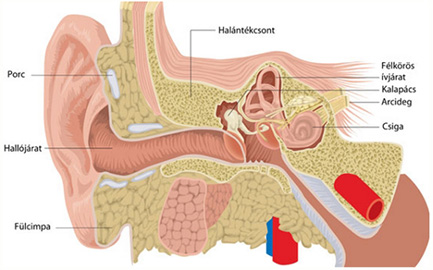
\includegraphics[width=4.51042in,height=2.8125in]{ful.jpg}}

\end{ajanlofig}

A füldugulás rendkívül gyakori tünet, a legtöbb esetben igen zavaró, de
ritkán akár fájdalmas is lehet. A füldugulás nem betegség, hanem
többféle betegség vagy probléma következtében kialakuló tünetről van
szó. Ennek megfelelően kezelését csak orvosi vizsgálat után lehet
elindítani, ha a füldugulást kiváltó okot sikerült azonosítani.

A füldugulás egyik leggyakoribb oka a fülzsír lerakódása!

\href{http://www.webbeteg.hu/cikkek/ful-orr-gegeszet/12276/a-fuldugulas-okai}{Részletek}

\end{ajanlo}

\begin{pelda}

Példák:

\begin{enumerate}
\def\labelenumi{\arabic{enumi}.}
\tightlist
\item
  \(\left. f:{\mathbb{R}}\rightarrowtail{\mathbb{R}},x \in {\mathbb{R}},x \geq 0,f\left( x \right) = x^{n},n \in {\mathbb{N}} \right.\),
  ekkor \(f\) szigorúan monoton nő,
  \(D_{f} = \left\lbrack {0,\infty} \right)\), \(f^{- 1}\) folytonos az
  \(y \in R_{f}\) pontokban és
  \(f^{- 1}\left( y \right) = \sqrt[n]{y}\). (Később látjuk a
  \protect\hyperlink{bolzanotetel}{Bolzano-tétellel}, hogy
  \(R_{f} = \left\lbrack {0,\infty} \right)\).)
\item
  \(\left. f:{\mathbb{R}}\rightarrowtail{\mathbb{R}},x \in {\mathbb{R}},f\left( x \right) = e^{x} \right.\),
  ekkor \(f\) szigorúan monoton nő, \(D_{f} = {\mathbb{R}}\),
  \(f^{- 1}\) folytonos. (Később látjuk a
  \protect\hyperlink{bolzanotetel}{Bolzano-tétellel}, hogy
  \(D_{f^{- 1}} = R_{f} = \left( {0,\infty} \right)\).)
\end{enumerate}

\end{pelda}

\begin{tetel}

Tétel:\\
Legyenek \(X\), \(Y\) metrikus terek,
\(\left. f:X\rightarrowtail Y,f \in C\left( D_{f} \right) \right.\),
\(D_{f}\) sorozatkompakt, \(f\) injektív
\(\left. \Rightarrow f^{- 1} \in C\left( R_{f} \right) \right.\).

\end{tetel}

\begin{bizonyitas}

Bizonyítás:\\
Legyen \(y_{0} \in D_{f^{- 1}} = R_{f}\). Belátjuk, hogy
\(f^{- 1} \in C\left\lbrack y_{0} \right\rbrack\). Alkalmazzuk az
átviteli elvet! Legyen \(y_{k} \in D_{f^{- 1}} = R_{f}\) olyan, amelyre
\(\lim\left( y_{k} \right) = y_{0}\). Belátandó:
\(\left. \left( {f^{- 1}\left( y_{k} \right)} \right)_{k \in {\mathbb{N}}}\rightarrow f^{- 1}\left( y_{0} \right) \right.\).
\[\left. x_{k}: = f^{- 1}\left( y_{k} \right),x_{0}: = f^{- 1}\left( y_{0} \right)\Rightarrow y_{k} = f\left( x_{k} \right),y_{0} = f{\left( x_{0} \right),} \right.\]
vagyis belátandó:
\(\left. \lim\left( x_{k} \right)\rightarrow x_{0} \right.\). Indirekt
bizonyítunk: ha ez nem lenne igaz, akkor
\(\exists\varepsilon_{0} > 0,x_{k_{l}}:\rho\left( {x_{k_{l}},x_{0}} \right) \geq \varepsilon_{0}\).
Tekintsük az \(\left( x_{k_{l}} \right)\) sorozatot, amelyre
\(x_{k_{l}} \in D_{f}\). Tudjuk, hogy \(D_{f}\) sorozatkompakt, ekkor
\(\exists\left( x_{k_{l_{j}}} \right):\lim\left( x_{k_{l_{j}}} \right) = x* \in D_{f}\),
de mivel
\(\left. f \in C\left\lbrack {x*} \right\rbrack\Rightarrow\underset{j\rightarrow\infty}{\lim}f\left( x_{k_{l_{j}}} \right) = f\left( {x*} \right) \right.\)
és mivel
\(\left. \underset{j\rightarrow\infty}{\lim}f\left( x_{k_{l_{j}}} \right) = \lim\left( y_{k_{l_{j}}} \right) = y_{0} = f\left( x_{0} \right)\Rightarrow f\left( x_{0} \right) = f\left( {x*} \right) \right.\).
De hát \(f\) injektív, vagyis \(x_{0} = x*\), ami meg ellentmondás, mert
\(\lim\left( x_{k_{l_{j}}} \right) = x* = x_{0}\) esetén
\(\exists j \in {\mathbb{N}}:\rho\left( {x_{k_{l_{j}}},x_{0}} \right) < \varepsilon_{0}\),
de ez ellentmond
\(\rho\left( {x_{k_{l}},x_{0}} \right) \geq \varepsilon_{0}\) -nak. ■

\end{bizonyitas}

\hypertarget{a-folytonos-fuggvenyek-alaptulajdonsagai}{%
\subsection{A folytonos függvények
alaptulajdonságai}\label{a-folytonos-fuggvenyek-alaptulajdonsagai}}

\begin{tetel}

Tétel:\\
Legyen \(X\), \(Y\) metrikus terek,
\(\left. f:X\rightarrow Y,f \in C\left( D_{f} \right) \right.\),
\(D_{f}\) sorozatkompakt \(\left. \Rightarrow R_{f} \right.\) is
sorozatkompakt. (Weierstrass tétele).

\end{tetel}

\begin{bizonyitas}

Bizonyítás:\\
Legyen \(\left( y_{k} \right) \subset R_{f}\) tetszőleges sorozat! Azt
kell megmutatni, hogy \(\exists\left( y_{k_{l}} \right)\) részsorozata,
mely konvergens és \(\lim\left( y_{k_{l}} \right) \in R_{f}\). Mivel
\(\left. y_{k} \in R_{f}\Rightarrow\exists x_{k} \in D_{f}:f\left( x_{k} \right) = y_{k} \right.\).
Mivel \(D_{f}\) sorozatkompakt és
\(\left. x_{k} \in D_{f}\Rightarrow\exists\left( x_{k_{l}} \right):\lim\left( x_{k_{l}} \right) = x_{0} \in D_{f} \right.\).
Mivel
\(\left. f \in C\left\lbrack x_{0} \right\rbrack\Rightarrow\underset{l\rightarrow\infty}{\lim}f\left( x_{k_{l}} \right) = f\left( x_{0} \right) = y_{0} \in R_{f} \right.\),
node \(f\left( x_{k_{l}} \right) = y_{k_{l}}\), ezért
\(\lim\left( y_{k_{l}} \right) = y_{0} \in R_{f}\), és pont ezt akartuk
belátni. ■

\end{bizonyitas}

Következmények:

\begin{enumerate}
\def\labelenumi{\arabic{enumi}.}
\tightlist
\item
  \(D_{f}\) sorozatkompakt \(\left. \Rightarrow R_{f} \right.\) korlátos
  és zárt (minden sorozatkompakt halmaz korlátos és zárt).
\item
  Ha \(Y = {\mathbb{R}}\) akkor is, ha \(D_{f}\) sorozatkompakt
  \(\left. \Rightarrow R_{f} \subset {\mathbb{R}} \right.\) korlátos és
  zárt. A korlátosság következménye: \(\sup R_{f},\inf R_{f}\) véges, és
  mivel az \(R_{f}\) értékkészlet zárt
  \(\left. \Rightarrow\exists x_{1},x_{2} \in D_{f}:f\left( x_{1} \right) = \inf f,f\left( x_{2} \right) = \sup f \right.\).
\end{enumerate}

\begin{pelda}

Példák:\\
Miért szükséges feltenni, hogy \(D_{f}\) sorozatkompakt (\(D_{f},R_{f}\)
sorozatkompaktsága \(\mathbb{R}\) -ben azt jelenti, hogy a halmazok
korlátosak és zártak):

\begin{enumerate}
\def\labelenumi{\arabic{enumi}.}
\tightlist
\item
  \(D_{f} = \left\lbrack {0,\infty} \right)\) zárt, de nem korlátos,
  \(f\left( x \right) = x\), ekkor
  \(R_{f} = \left\lbrack {0,\infty} \right)\) nem korlátos.
\item
  \(D_{f} = \left( 0,1 \right\rbrack,f\left( x \right) = \frac{1}{x}\),
  ekkor \(D_{f}\) korlátos, de nem zárt, \(R_{f}\) pedig nem korlátos.
\end{enumerate}

\end{pelda}

\begin{megjegyzes}

Megjegyzés:\\
Az a tény, hogy egy
\[\left. f:X\rightarrowtail Y,f \in C\left\lbrack x_{0} \right\rbrack\Rightarrow\forall\varepsilon > 0\exists\delta > 0:x \in B_{\delta}\left( x_{0} \right) \cap D_{f}\Rightarrow f\left( x \right) \in B_{\varepsilon}{\left( {f\left( x_{0} \right)} \right),} \right.\]
ahol \(\delta\) függhet \(\varepsilon\)-tól és \(x_{0}\)-tól is.

\end{megjegyzes}

\begin{definicio}

Definíció:\\
Azt mondjuk, hogy \(X\), \(Y\) metrikus terek esetén egy
\(\left. f:X\rightarrowtail Y \right.\) függvény egyenletesen folytonos,
ha
\[\left. \forall\varepsilon > 0\exists\delta > 0:x_{1},x_{2} \in D_{f},\rho\left( {x_{1},x_{2}} \right) < \delta\Rightarrow\rho\left( {f\left( x_{1} \right),f\left( x_{2} \right)} \right) < \varepsilon. \right.\]
Tehát ekkor \(\delta\) csak \(\varepsilon\)-tól függ.

\end{definicio}

\begin{tetel}

Tétel (Heine tétele):\\
Ha \(f\) folytonos és \(D_{f}\) sorozatkompakt
\(\left. \Rightarrow f \right.\) egyenletesen folytonos.

\end{tetel}

\begin{bizonyitas}

Bizonyítás:\\
Tfh \(f\) folytonos, \(D_{f}\) sorozatkompakt. Indirekt bizonyítunk:
\(\exists\varepsilon > 0\forall\delta > 0:\exists x_{1},x_{2} \in D_{f},\rho\left( {x_{1},x_{2}} \right) < \delta\),
de
\(\rho\left( {f\left( x_{1} \right),f\left( x_{2} \right)} \right) \geq \varepsilon\).
Legyen \(\delta: = \frac{1}{k},k \in {\mathbb{N}}\), ekkor tehát
\(\exists x_{k},\widetilde{x_{k}} \in D_{f}:\rho\left( {x_{k},\widetilde{x_{k}}} \right) < \frac{1}{k}\)
de
\(\rho\left( {f\left( x_{k} \right),f\left( \widetilde{x_{k}} \right)} \right) \geq \varepsilon\).
Tudjuk, hogy \(D_{f}\) sorozatkompakt, így
\(\exists\left( x_{k_{l}} \right) \subset D_{f}:\lim\left( x_{k_{l}} \right) = x_{0} \in D_{f}\).
Mivel
\(\left. \rho\left( {x_{k_{l}},\widetilde{x_{k_{l}}}} \right) < \frac{1}{k},\lim\left( \frac{1}{k} \right) = 0\Rightarrow\lim\left( \widetilde{x_{k_{l}}} \right) = \lim\left( x_{k_{l}} \right) = x_{0} \in D_{f} \right.\).
Mivel \(f \in C\left\lbrack x_{0} \right\rbrack\), az átviteli elv
alapján
\(\left. \Rightarrow\underset{l\rightarrow\infty}{\lim}f\left( x_{k_{l}} \right) = f\left( x_{0} \right),\underset{l\rightarrow\infty}{\lim}f\left( \widetilde{x_{k_{l}}} \right) = f\left( x_{0} \right) \right.\),
de ez meg ellentmondás a feltevésünkkel, miszerint
\(\rho\left( {f\left( x_{k} \right),f\left( \widetilde{x_{k}} \right)} \right) \geq \varepsilon\).
■

\end{bizonyitas}

\begin{pelda}

Példák:

\begin{enumerate}
\def\labelenumi{\arabic{enumi}.}
\tightlist
\item
  \(D_{f} = \left\lbrack {0,\infty} \right)\) ez zárt, de nem korlátos,
  \(f\left( x \right): = x^{2}\) nem egyenletesen folytonos.
\item
  \(D_{f} = \left( 0,1 \right\rbrack\) ez korlátos, de nem zárt,
  \(f\left( x \right): = \frac{1}{x}\) nem egyenletesen folytonos.
\end{enumerate}

\end{pelda}

\begin{tetel}

Tétel (Bolzano-tétel):\protect\hypertarget{bolzanotetel}{}{}\\
Legyen
\(\left. f:\left\lbrack {a,b} \right\rbrack\rightarrow{\mathbb{R}},f \in C\left\lbrack {a,b} \right\rbrack,f\left( a \right) \neq f\left( b \right) \right.\),
ekkor tetszőleges
\(\eta \in \left( {f\left( a \right),f\left( b \right)} \right)\)
számhoz
\(\exists\xi \in \left( {a,b} \right):f\left( \xi \right) = \eta\).

\end{tetel}

\begin{bizonyitas}

Bizonyítás:

tekintsük a következő halmazt:
\(\left. M: = \left\{ {x \in \left\lbrack {a,b} \right\rbrack:f\left( x \right) < \eta} \right\} \subset \left\lbrack {a,b} \right\rbrack\Rightarrow M \neq \varnothing \right.\)
mivel \(a \in M\), továbbá \(M\) korlátos. Legyen \(\xi: = \sup M\).
Belátjuk, hogy \(f\left( \xi \right) = \eta\). Indirekt bizonyítunk:
\(f\left( \xi \right) < \eta\) vagy \(f\left( \xi \right) > \eta\) nem
lehetséges.

Első eset: ha \(f\left( \xi \right) < \eta\) lenne, akkor
\(\left. f\left( b \right) > \eta\Rightarrow\xi \neq b \right.\), ezért
\(\xi\) -nek megadható olyan jobboldali környezete, ahol a
függvényértékek \(\eta\) -nál kisebbek, mert
\(f \in C\left\lbrack \xi \right\rbrack\), vagyis
\(\left. \exists\delta > 0:x \in \left\lbrack {\xi,\xi + \delta} \right\rbrack\Rightarrow f\left( x \right) < \eta \right.\),
ez pedig ellentmond annak, hogy \(\xi = \sup M\).

Második eset: ha \(f\left( \xi \right) > \eta\) lenne, akkor
\(\left. f\left( a \right) < \eta\Rightarrow\xi \neq a \right.\) és
\[\left. f \in C\left\lbrack {a,b} \right\rbrack\Rightarrow\exists\delta > 0:x \in \left\lbrack {\xi - \delta,\xi} \right\rbrack\Rightarrow f\left( x \right) > \eta. \right.\]
Ez is ellentmond annak, hogy
\(\xi = \sup M = \sup\left\{ {x \in \left\lbrack {a,b} \right\rbrack:f\left( {x < \eta} \right)} \right\}\).
Tehát mivel
\(\left. f\left( \xi \right) \ngtr \eta,f\left( \xi \right) \nless \eta\Rightarrow f\left( \xi \right) = \eta \right.\).
■

\end{bizonyitas}

Következmények: legyen \(I \subset {\mathbb{R}}\) valamilyen intervallum
(véges vagy végtelen, nyílt vagy zárt), és tfh
\(\left. f:I\rightarrow{\mathbb{R}},f \in C\left( I \right) \right.\).
Ekkor
\(\forall x_{1},x_{2} \in I,y \in \left( {f\left( x_{1} \right),f\left( x_{2} \right)} \right)\)
esetén
\(\exists x_{0} \in \left( {x_{1},x_{2}} \right):f\left( x_{0} \right) = y\).

\begin{megjegyzes}

Megjegyzés:\\
Az ilyen tulajdonságú függvényeket Darboux tulajdonságúaknak nevezzük. A
Bolzano-tétel kimondja, hogy ha
\(\left. f:I\rightarrow{\mathbb{R}},f \in C\left( I \right)\Rightarrow \right.\)
\(f\) Darboux tulajdonságú.

\end{megjegyzes}

\begin{pelda}

Példa: \[f\left( x \right) = \begin{cases}
{\sin\frac{1}{x}} & {\text{ha~}0 < x \leq 1} \\
0 & {\text{ha~}x = 0.} \\
\end{cases}\] Ez a függvény Darboux tulajdonságú, de nem folytonos
0-ban.

\end{pelda}

\begin{allitas}

Állítás:\\
Egy \(A \subset {\mathbb{R}}\) halmaz intervallum
\(\left. \Leftrightarrow\forall x_{1},x_{2} \in A,\forall x \in \left( {x_{1},x_{2}} \right) \right.\)
esetén \(x \in A\).

\end{allitas}

Ezen állítás segítségével a Bolzano-tétel így is megfogalmazható:

\begin{tetel}

Tétel:\\
Ha \(I\) intervallum, és
\(\left. f:I\rightarrow{\mathbb{R}},f \in C\left( I \right)\Rightarrow R_{f} \right.\)
is intervallum.

\end{tetel}

Alkalmazás:

\begin{enumerate}
\def\labelenumi{\arabic{enumi}.}
\tightlist
\item
  \(I: = \left\lbrack {0,\infty} \right),f\left( x \right) = x^{n},n \in {\mathbb{N}}\)!
  Ekkor a tétel szerint mivel \(f\) folytonos, \(R_{f}\) valamilyen
  intervallum, \(f\) szigorúan monoton nő,
  \[\left. f\left( 0 \right) = 0,\underset{x\rightarrow\infty}{\lim}f\left( x \right) = \infty\Rightarrow R_{f} = \left\lbrack {0,\infty} \right)\Rightarrow D_{f^{- 1}} = {\left\lbrack {0,\infty} \right).} \right.\]
\item
  \(\left. I = {\mathbb{R}},f:I\rightarrow{\mathbb{R}},f\left( x \right) = e^{x}\Rightarrow f\left( x \right) \in C\left( I \right),\underset{x\rightarrow - \infty}{\lim}f\left( x \right) = 0,\underset{x\rightarrow\infty}{\lim}f\left( x \right) = \infty \right.\).
  Itt \(f\) szigorúan monoton nő,
  \(\left. R_{f} = \left( {0,\infty} \right)\Rightarrow D_{f^{- 1}} \equiv D_{\ln} = \left( {0,\infty} \right) \right.\).
\end{enumerate}

\begin{ajanlo}

\begin{ajanlofig}

\href{https://en.wikipedia.org/wiki/World_Wide_Fund_for_Nature}{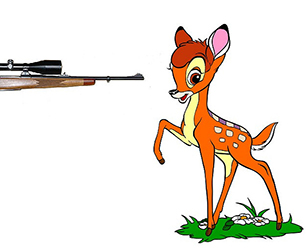
\includegraphics[width=3.19792in,height=2.60417in]{bambi.jpg}}

\end{ajanlofig}

Szegény Bambira fegyvert fognak. Miért sajnálod, pedig az őzek nem is
védett állatok?! Vannak azonban olyan fajok, amelyet a kihalás fenyeget.

The \textbf{World Wide Fund for Nature} (\textbf{WWF}) is an
\href{https://en.wikipedia.org/wiki/Internationalism_(politics)}{international}
\href{https://en.wikipedia.org/wiki/Non-governmental_organization}{non-governmental
organization} founded in 1961, working in the field of the wilderness
preservation, and the reduction of
\href{https://en.wikipedia.org/wiki/Human_impact_on_the_environment}{human
impact on the environment}. It was formerly named the \textbf{World
Wildlife Fund}, which remains its official name in
\href{https://en.wikipedia.org/wiki/Canada}{Canada} and the
\href{https://en.wikipedia.org/wiki/United_States}{United States}. The
\href{https://en.wikipedia.org/wiki/Living_Planet_Report}{Living Planet
Report} is published every two years by WWF since 1998; it is based on a
\href{https://en.wikipedia.org/wiki/Living_Planet_Index}{Living Planet
Index} and
\href{https://en.wikipedia.org/wiki/Ecological_footprint}{ecological
footprint} calculation.

It is the world's largest
\href{https://en.wikipedia.org/wiki/Conservation_organization}{conservation
organization} with over five million supporters worldwide, working in
more than 100 countries, supporting around
1,300\href{https://en.wikipedia.org/wiki/World_Wide_Fund_for_Nature\#cite_note-4}{{[}4{]}}
conservation and environmental projects. WWF is a
foundation,\href{https://en.wikipedia.org/wiki/World_Wide_Fund_for_Nature\#cite_note-5}{{[}5{]}}
with 55\% of funding from individuals and bequests, 19\% from government
sources (such as the
\href{https://en.wikipedia.org/wiki/World_Bank}{World Bank},
\href{https://en.wikipedia.org/wiki/Department_for_International_Development}{DFID},
\href{https://en.wikipedia.org/wiki/United_States_Agency_for_International_Development}{USAID})
and 8\% from corporations in
2014.\href{https://en.wikipedia.org/wiki/World_Wide_Fund_for_Nature\#cite_note-WWF-INT_Annual_Review-6}{{[}6{]}}

\end{ajanlo}

\hypertarget{bolzano-tetel-metrikus-terekben}{%
\subsubsection{Bolzano-tétel metrikus
terekben}\label{bolzano-tetel-metrikus-terekben}}

\begin{definicio}

Definíció:\\
Legyen \(X\) metrikus tér,
\(\left. \left\lbrack {\alpha,\beta} \right\rbrack \subset {\mathbb{R}},\varphi:\left\lbrack {\alpha,\beta} \right\rbrack\rightarrow X,\varphi \in C\left\lbrack {\alpha,\beta} \right\rbrack \right.\).
Ekkor azt mondjuk, hogy \(\varphi\) folytonos ívet, görbét határoz meg
az \(X\)-ben.
\(R_{\varphi} = \left\{ {\varphi\left( t \right):t \in \left\lbrack {\alpha,\beta} \right\rbrack} \right\} \subset X\).
Ekkor \(\varphi\left( \alpha \right)\) és
\(\varphi\left( \beta \right)\)-t a görbe végpontjainak nevezzük. (Megj:
van, amikor \(\varphi\) -t nevezzük görbének, nem pedig a "képét".)

\end{definicio}

\begin{definicio}

Definíció:\\
Azt mondjuk, hogy az \(A \subset X\) halmaz ívszerűen összefüggő, ha az
\(A\) halmaz bármely két pontja összeköthető az \(A\)-ban haladó
folytonos görbével, ívvel, vagyis
\(\left. \forall a,b \in A\exists\varphi:\left\lbrack {\alpha,\beta} \right\rbrack\rightarrow X,\varphi \in C\left\lbrack {\alpha,\beta} \right\rbrack \right.\),
hogy
\[\left. \varphi\left( \alpha \right) = a,\varphi\left( \beta \right) = b,t \in \left( {\alpha,\beta} \right)\Rightarrow\varphi\left( t \right) \in A \right..\]

\end{definicio}

\begin{tetel}

Tétel:\\
Legyenek \(X\), \(Y\) metrikus terek,
\(\left. f:X\rightarrowtail Y,f \in C\left( D_{f} \right) \right.\) ! Ha
\(D_{f}\) ívszerűen összefüggő, akkor \(R_{f}\) is.

\end{tetel}

\begin{bizonyitas}

Bizonyítás:\\
Legyenek \(y_{1},y_{2} \in R_{f}\). Belátjuk, hogy \(y_{1},y_{2}\)
összeköthető \(R_{f}\)-ben haladó folytonos ívvel. Mivel
\[\left. y_{1},y_{2} \in R_{f}\Rightarrow\exists x_{1},x_{2} \in D_{f}:f\left( x_{1} \right) = y_{1},f\left( x_{2} \right) = y_{2} \right..\]
Mivel \(D_{f}\) ívszerűen összefüggő
\[\left. \Rightarrow\exists\varphi:\left\lbrack {\alpha,\beta} \right\rbrack\rightarrow X,\varphi \in C\left\lbrack {\alpha,\beta} \right\rbrack \right.\]
úgy, hogy
\[\left. \varphi\left( \alpha \right) = x,\varphi\left( \beta \right) = x_{2},t \in \left( {\alpha,\beta} \right)\Rightarrow\varphi\left( t \right) \in D_{f}. \right.\]
Legyen
\(\left. \psi:\left\lbrack {\alpha,\beta} \right\rbrack\rightarrow Y,\psi: = f \circ \varphi \right.\)
ekkor \(\psi\) folytonos (kompozíció függvény tulajdonságából), továbbá
\(\left. t \in \left( {\alpha,\beta} \right)\Rightarrow\psi\left( t \right) = f\left( {\varphi\left( t \right)} \right) \in R_{f} \right.\),
sőt,
\[\psi\left( \alpha \right) = f\left( {\varphi\left( \alpha \right)} \right) = f\left( x_{1} \right) = y_{1},\psi\left( \beta \right) = f\left( {\varphi\left( \beta \right)} \right) = f\left( x_{2} \right) = y_{2}.\]
■

\end{bizonyitas}

\begin{definicio}

Definíció:\\
Azt mondjuk, hogy az \(A \subset X\) összefüggő
(\href{https://hu.wikipedia.org/wiki/Topol\%C3\%B3gia}{topológiai}
értelemben), ha nem adható meg \(G_{1}\) és \(G_{2}\) diszjunkt nyílt
halmaz úgy, hogy
\(G_{1} \cup G_{2} \supset A,A \cap G_{1} \neq \varnothing,A \cap G_{2} \neq \varnothing\).

\end{definicio}

\begin{megjegyzes}

Megjegyzés:\\
belátható, hogy ha \(A\) ívszerűen összefüggő, akkor összefüggő.

\end{megjegyzes}

\begin{tetel}

Tétel (Bolzano-tétel metrikus térben, bizonyítás nélkül):\\
Legyenek \(X\), \(Y\) metrikus terek,
\(\left. f:X\rightarrowtail Y,f \in C\left( D_{f} \right) \right.\) ! Ha
\(D_{f}\) összefüggő \(\left. \Rightarrow R_{f} \right.\) is.

\end{tetel}

\hypertarget{fuggvenysorok-es-sorozatok-egyenletes-konvergenciaja}{%
\subsubsection{Függvénysorok és sorozatok egyenletes
konvergenciája}\label{fuggvenysorok-es-sorozatok-egyenletes-konvergenciaja}}

\begin{definicio}

Definíció:\\
Legyenek \(X\), \(Y\) metrikus terek, \(M \subset X\), és
\(\forall j \in {\mathbb{N}}\)-re
\(\left. f_{j}:M\rightarrow Y \right.\). Azt mondjuk, hogy \(f_{j}\)
függvények függvénysorozatot alkotnak, jelölése
\(\left( f_{j} \right)_{j \in {\mathbb{N}}}\).

\end{definicio}

\begin{definicio}

Definíció:\\
Azt mondjuk, hogy az \(\left. f_{j}:M\rightarrow Y \right.\)
függvényekből álló sorozat pontonként tart egy
\(\left. f:M\rightarrow Y \right.\) függvényhez, ha
\(\forall x \in M,\underset{j\rightarrow\infty}{\lim}f_{j}\left( x \right) = f\left( x \right)\).

\end{definicio}

Kérdés: feltéve, hogy \(f_{j} \in C\left( M \right)\) minden \(j\)-re,
\(\left. \Rightarrow f \in C\left( M \right) \right.\) ? Általában nem.
Pl:
\(f_{j}\left( x \right) = x^{j},0 \leq x \leq 1,j \in {\mathbb{N}}\),
ekkor \(\forall f_{j} \in C\left( M \right)\), de
\[\underset{j\rightarrow\infty}{\lim}f_{j}\left( x \right) = \begin{cases}
0 & {\text{ha~}0 \leq x < 1} \\
1 & {\text{ha~}x = 1.} \\
\end{cases}\]

\begin{definicio}

Definíció:\\
Azt mondjuk, hogy az \(\left. f_{j}:M\rightarrow Y \right.\)
függvényekből álló sorozat egyenletesen tart az
\(\left. f:M\rightarrow Y \right.\) függvényhez, ha
\[\left. \forall\varepsilon > 0\exists j_{0} \in {\mathbb{N}}:j > j_{0}\Rightarrow\rho\left( {f_{j}\left( x \right),f\left( x \right)} \right) < \varepsilon,\forall x \in M. \right.\]

\end{definicio}

\begin{megjegyzes}

Megjegyzés:\\
\(j_{0}\) csak \(\varepsilon\)-tól függ, és nem függ \(x\)-től.
(Pontonkénti konvergencia esetén függhet \(x\)-től.)

\end{megjegyzes}

\begin{pelda}

Példa:\\
\(f_{j}\left( t \right): = t^{j},0 < a < 1,0 \leq t \leq a\), ekkor
\(f_{j}\) egyenletesen tart 0-hoz a
\(\left\lbrack {0,a} \right\rbrack\)-n. Ugyanis legyen
\(\varepsilon > 0\) tetszőleges, \(0 \leq t^{j} < \varepsilon\) esetén
\(0 \leq t^{j} < \varepsilon\) mikor teljesül? Válasszuk meg \(j_{0}\)
számot úgy, hogy \(j > j_{0}\) esetén \(a^{j} < \varepsilon\). Ezt
mindig megtehetjük, ugyanis \(0 < a < 1\), így \(0 \leq t \leq a\)
esetén \(t^{j} \leq a^{j} \leq \varepsilon\).

\end{pelda}

\begin{tetel}

Tétel:\\
Legyen
\(\left. f_{j}:M\rightarrow Y,M \subset X,f_{j} \in C\left( D_{f} \right) \right.\).
Ha \(\left( f_{j} \right)\) függvénysorozat egyenletesen tart egy
\(\left. f:M\rightarrow Y \right.\) függvényhez, akkor \(f\) folytonos.

\end{tetel}

\begin{bizonyitas}

Bizonyítás:\\
Legyen \(x_{0} \in M\). Belátjuk, hogy
\(f \in C\left\lbrack x_{0} \right\rbrack\). Tetszőleges \(x \in M\)
esetén
\[{\rho\left( {f\left( x \right),f\left( x_{0} \right)} \right) \leq \rho\left( {f\left( x \right),f_{j}\left( x \right)} \right) + \rho\left( {f_{j}\left( x \right),f_{j}\left( x_{0} \right)} \right) + \rho\left( {f_{j}\left( x_{0} \right),f\left( x_{0} \right)} \right)}.\]
Legyen \(\frac{\varepsilon}{3} > 0\) tetszőleges, ezért mivel
\(\left( f_{j} \right)\) egyenletesen tart \(f\)-hez,
\[\left. \exists j_{0}:j > j_{0}\Rightarrow\rho\left( {f\left( x \right),f_{j}\left( x \right)} \right) < \frac{\varepsilon}{3},\rho\left( {f\left( x_{0} \right),f_{j}\left( x_{0} \right)} \right) < \frac{\varepsilon}{3}. \right.\]
Választhatunk egy rögzített \(j > j_{0}\)-t, mondjuk \(j = j_{0} + 1\).
Továbbá tudjuk, hogy
\[\left. f_{j} \in C\left\lbrack x_{0} \right\rbrack\Rightarrow\exists\delta > 0:x \in M,\rho\left( {x,x_{0}} \right) < \delta\Rightarrow\rho\left( {f_{j}\left( x \right),f_{j}\left( x_{0} \right)} \right) < \frac{\varepsilon}{3}. \right.\]
tehát
\[\rho \left( {f\left( x \right),f\left( {{x_0}} \right)} \right) \leqslant \underbrace {\rho \left( {f\left( x \right),{f_j}\left( x \right)} \right)}_{ < \varepsilon /3{\text{\;mivel\;}}j > {j_0}} + \underbrace {\rho \left( {{f_j}\left( x \right),{f_j}\left( {{x_0}} \right)} \right)}_{ < \varepsilon /3{\text{\;ha\;}}x \in {B_\delta }\left( {{x_0}} \right)} + \underbrace {\rho \left( {{f_j}\left( {{x_0}} \right),f\left( {{x_0}} \right)} \right)}_{ < \varepsilon /3{\text{ mivel }}j > {j_0}} < \varepsilon .\]
■

\end{bizonyitas}

\begin{megjegyzes}

Megjegyzés:\\
\(f_{j}\left( t \right): = t^{j},0 \leq t \leq 1\) függvények esetén
\(\left( f_{j} \right)\) függvénysorozat nem tart egyenletesen az \(f\)
függvényhez.

\end{megjegyzes}

\begin{definicio}

Definíció:\\
Legyen \(X\) metrikus tér,
\(\left. Y = {\mathbb{R}},M \subset X,g_{k}:M\rightarrow{\mathbb{R}} \right.\)
(\(\mathbb{R}\) helyett lehetne \(\mathbb{C}\) is). Ekkor tekintsük a
következő függvénysorozatot:
\(f_{j}: = {\sum\limits_{k = 1}^{j}g_{k}}\). Az ilyen módon értelmezett
\(\left( f_{j} \right)\) sorozatot a \(g_{k}\) tagokból álló
függvénysornak nevezzük.

\end{definicio}

\begin{definicio}

Definíció:\\
Azt mondjuk, hogy a \(g_{k}\) tagokból álló függvénysor pontonként
konvergens és összege az \(\left. f:M\rightarrow{\mathbb{R}} \right.\)
függvény, ha \(\forall x \in M\) esetén \(g_{k}\left( x \right)\)
tagokból álló számsor konvergens \(\mathbb{R}\)-ben, és a sor összege
\(f\left( x \right)\), és ezt így jelöljük:
\({\sum\limits_{k = 1}^{\infty}{g_{k}\left( x \right)}} = f\left( x \right)\)
jelöljük.\\
Megjegyzés:
\({\sum\limits_{k = 1}^{\infty}{g_{k}\left( x \right) \equiv \underset{j\rightarrow\infty}{\lim}}}f_{j}\left( x \right) = \underset{j\rightarrow\infty}{\lim}{\sum\limits_{k = 1}^{j}{g_{j}\left( x \right)}}\).

\end{definicio}

\begin{definicio}

Definíció:\\
Azt mondjuk, hogy a \(\left( g_{k} \right)\) tagokból álló függvénysor
egyenletesen konvergál egy \(\left. f:M\rightarrow{\mathbb{R}} \right.\)
függvényhez, ha \(f_{j} = {\sum\limits_{k = 1}^{j}g_{k}}\) esetén
\(\left( f_{j} \right)\) függvénysorozat egyenletesen tart \(f\)-hez.

\end{definicio}

\begin{tetel}

Tétel:\\
Tfh \(\left. g_{k}:M\rightarrow{\mathbb{R}} \right.\) folytonos és a
\(g_{k}\) tagokból álló sor egyenletesen konvergál egy
\(\left. f:M\rightarrow{\mathbb{R}} \right.\) függvényhez
\(\left. \Rightarrow f \in C\left( D_{f} \right) \right.\).

\end{tetel}

\begin{bizonyitas}

Bizonyítás:\\
\(f_{j} = {\sum\limits_{k = 1}^{j}g_{k}}\) folytonos,
\(\lim\left( f_{j} \right) = f\)-hez egyenletesen konvergál
\(\left. \Rightarrow f \in C\left( D_{f} \right) \right.\).■

\end{bizonyitas}

\begin{tetel}

Tétel (Weierstrass-kritérium):\\
Tfh \(\left. g_{k}:M\rightarrow{\mathbb{R}} \right.\) függvényekre
teljesül, hogy
\(\left| g_{k} \right| \leq a_{k},a_{k} \in {\mathbb{R}}\) és
\({\sum\limits_{k = 1}^{\infty}a_{k}} < \infty\). Ekkor a
\(\left( g_{k} \right)\) tagokból álló függvénysor egyenletesen
konvergens.

\end{tetel}

\begin{bizonyitas}

Bizonyítás:

legyen \(x \in M\) tetszőleges, rögzített pont. Először belátjuk, hogy
\(\sum\limits_{k = 1}^{\infty}{\left| {g_{k}\left( x \right)} \right| < \infty}\).
Legyen
\(f_{j}\left( x \right): = {\sum\limits_{k = 1}^{j}{g_{k}\left( x \right)}}\),
ekkor
\[\left. \exists j_{0}:j > l > j_{0}\Rightarrow\left| {f_{j}\left( x \right) - f_{l}\left( x \right)} \right| = \left| {\sum\limits_{k = l + 1}^{j}{g_{k}\left( x \right)}} \right| \leq {\sum\limits_{k = l + 1}^{j}\left| {g_{k}\left( x \right)} \right|} \leq {\sum\limits_{k = l + 1}^{j}a_{k}} < \varepsilon, \right.\]
mivel \({\sum\limits_{k = 1}^{\infty}a_{k}} < \infty\), vagyis
\(\left( {f_{j}\left( x \right)} \right)_{j \in {\mathbb{N}}}\)
számsorozatra teljesül a Cauchy-kritérium. Mivel \(\mathbb{R}\) teljes
tér
\(\left. \Rightarrow\exists f\left( x \right) \in {\mathbb{R}}:\underset{j\rightarrow\infty}{\lim}f_{j}\left( x \right) = f\left( x \right) \right.\),
vagyis a \(\left| {g_{k}\left( x \right)} \right|\) és a
\(g_{k}\left( x \right)\) tagokból álló függvénysor konvergens.

Most belátjuk, hogy a sor, illetve a vele ekvivalens
\(\left( f_{j} \right)\) függvénysorozat egyenletesen konvergál \(f\)
-hez. Legyen \(\varepsilon > 0\) tetszőleges, a fentiek szerint,
\(\left. j\rightarrow\infty \right.\) határátmenetben a fenti
egyenlőtlenségből kapjuk, hogy
\(\left| {f\left( x \right) - f_{l}\left( x \right)} \right| \leq {\sum\limits_{k = l + 1}^{\infty}a_{k}} < \varepsilon,\forall x \in M\),
ha \(l > j_{0}\). De hisz ez pont az jelenti, hogy \(f_{k}\)
egyenletesen tart \(f\) -hez. ■

\end{bizonyitas}

\hypertarget{hatvanysorok}{%
\subsection{Hatványsorok}\label{hatvanysorok}}

\begin{definicio}

Definíció:\\
Egy
\(c_{j}x^{j},x \in {\mathbb{R}},c_{j} \in {\mathbb{R}},j = 0,1,2...\)
tagokból álló függvénysort hatványsornak nevezünk.

\end{definicio}

\begin{megjegyzes}

Megjegyzés:\\
A hatványsor tagjai folytonos függvények.

\end{megjegyzes}

Kérdés: a hatványsor mely \(x\) -ekre konvergens, illetve egyenletesen
konvergens?

\begin{definicio}

Definíció:\\
Legyen \(a_{k} \in {\mathbb{R}},k \in {\mathbb{R}}\). Az
\(\left( a_{k} \right)_{k \in {\mathbb{N}}}\) valós számsorozat limesz
szuperiorját illetve limesz inferiorját így értelmezzük:
\(\lim\sup\left( a_{k} \right)_{k \in {\mathbb{N}}} = \underset{k\rightarrow\infty}{\lim\sup}a_{k}\)
jelenti azt a legnagyobb valós számot (vagy végtelent), amelyhez az
\(\left( a_{k} \right)\) egy alkalmas részsorozata konvergál. Ezzel
analóg a \(\lim\inf\left( a_{k} \right)\).

\end{definicio}

\begin{megjegyzes}

Megjegyzés:

\begin{enumerate}
\def\labelenumi{\arabic{enumi}.}
\tightlist
\item
  Mindig létezik limesz inferior és limesz szuperior.
\item
  Ha
  \(\left. \exists\lim\left( a_{k} \right)\Rightarrow\lim\left( a_{k} \right) = \lim\sup\left( a_{k} \right) = \lim\inf\left( a_{k} \right) \right.\)
  .
\item
  \(\lim\sup\left( a_{k} \right) = \underset{k\rightarrow\infty}{\lim}\left\lbrack {\sup\left\{ {a_{k},a_{k + 1},...} \right\}} \right\rbrack\)
  .
\end{enumerate}

\end{megjegyzes}

\begin{tetel}

Tétel:\\
Legyen \(R: = \frac{1}{\lim\sup\sqrt[k]{\left| c_{k} \right|}}\). Ha a
nevező nulla lenne, akkor \(R: = \infty\), ha végtelen, akkor
\(R: = 0\). Ekkor \(\left| x \right| < R\) esetén a hatványsor
konvergens, \(\left| x \right| > R\) esetén pedig divergens.

\end{tetel}

\begin{bizonyitas}

Bizonyítás:\\
A gyökkritérium alapján\ldots{}

\end{bizonyitas}

\begin{tetel}

Tétel:\\
Legyen \(0 < R_{0} < R\), ekkor a hatványsor egyenletesen konvergens az
\(R_{0}\) sugarú intervallumban (vagy körben).

\end{tetel}

\begin{bizonyitas}

Bizonyítás:\\
Weierstrass-kritériummal bizonyítjuk. Legyen
\(g_{j}\left( x \right) = c_{j}x^{j},j = 0,1,...\), ekkor
\(\left| {g_{j}\left( x \right)} \right| = \left| {c_{j}x^{j}} \right| = \left| c_{j} \right|\left| x^{j} \right| \leq \left| c_{j} \right|R_{0}^{j}\).
Azt kellene belátni, hogy \(\left| c_{j} \right|R_{0}^{j}\) tagokból
álló sor konvergens. Alkalmazzuk erre a gyökkritériumot!
\[\left. \sqrt[j]{\left| c_{j} \right|R_{0}^{j}} = R_{0}\sqrt[j]{\left| c_{j} \right|},\underset{j\rightarrow\infty}{\lim\sup}\sqrt[j]{\left| c_{j} \right|R_{0}^{j}} = R_{0}\underset{j\rightarrow\infty}{\lim\sup}\sqrt[j]{\left| c_{j} \right|} = \frac{R_{0}}{R} < 1\Rightarrow{\sum\limits_{j = 1}^{\infty}{\left| c_{j} \right|R_{0}^{j}}} \right.\]
konvergens (ez a gyökkritérium). ■

\end{bizonyitas}

Következmény: a hatványsor összege folytonos a konvergenciakör
belsejében. Például
\(e^{x} = {\sum\limits_{j = 0}^{\infty}\frac{x^{j}}{j!}}\), ennek a
konvergencia-sugara végtelen, mert
\[{R = \frac{1}{\lim\sup\sqrt[n]{1/n!}} = \lim\sup\sqrt[n]{n!} = \infty}.\]

\begin{ajanlo}

\begin{ajanlofig}

\href{https://hu.wikipedia.org/wiki/Csell\%C3\%B3}{
\includegraphics[width=3.80208in,height=2.13542in]{cello.jpg}}

\end{ajanlofig}

A \textbf{cselló} (\textbf{gordonka}, \textbf{kisbőgő}) egy nagy
hangterjedelmű, \href{https://hu.wikipedia.org/wiki/Basszus}{basszus}
fekvésű
\href{https://hu.wikipedia.org/wiki/Von\%C3\%B3s_hangszerek}{vonós}
\href{https://hu.wikipedia.org/wiki/Hangszer}{hangszer}, és hasonlóan e
\href{https://hu.wikipedia.org/wiki/Hangszercsal\%C3\%A1d}{hangszercsalád}
(hegedűcsalád) többi tagjához, vagyis a
\href{https://hu.wikipedia.org/wiki/Heged\%C5\%B1}{hegedűhöz}, a
\href{https://hu.wikipedia.org/wiki/Br\%C3\%A1csa}{brácsához} és a
\href{https://hu.wikipedia.org/wiki/Nagyb\%C5\%91g\%C5\%91}{nagybőgőhöz},
ez a hangszer is négy húrral rendelkezik, melyek
\href{https://hu.wikipedia.org/wiki/Kvint}{kvint} távolságra vannak
egymástól. A nagybőgő és a mélyhegedű közt a középső helyet foglalja el
alakjára és hangterjedelmére nézve.

\end{ajanlo}

\hypertarget{differencialhatosag}{%
\section{Differenciálhatóság}\label{differencialhatosag}}

\begin{definicio}

Definíció:\\
Egy \(\left. f:{\mathbb{R}}\rightarrowtail{\mathbb{R}} \right.\) vagy
\(\left. {\mathbb{C}}\rightarrowtail{\mathbb{C}} \right.\) függvényt az
\(x_{0}\) pontban differenciálhatónak nevezünk, ha
\(x_{0} \in {int}D_{f}\) és
\(\exists\underset{x\rightarrow x_{0}}{\lim}\frac{f\left( x \right) - f\left( x_{0} \right)}{x - x_{0}}\)
és véges
\(\left. \Leftrightarrow\exists\underset{\varepsilon\rightarrow 0}{\lim}\frac{f\left( {x_{0} + \varepsilon} \right) - f\left( x_{0} \right)}{\varepsilon} \right.\)
és véges.

\end{definicio}

\begin{megjegyzes}

Megjegyzés:\\
Hogy egy ilyen definíciót továbbvihessünk "többváltozós" függvényekre,
szükségünk van a lineáris leképezések vizsgálatára.

\end{megjegyzes}

\hypertarget{linearis-lekepezesek}{%
\subsection{Lineáris leképezések}\label{linearis-lekepezesek}}

\begin{definicio}

Definíció:\\
Legyen \(X\) vektortér, azt mondjuk, hogy az \(M \subset X\) halmaz
elemei lineárisan függetlenek, ha bármely \(M\)-beli véges sok elemre
\(\left. {\sum\limits_{i}{\alpha_{i}x_{i}}} = 0\Leftrightarrow\alpha_{i} = 0 \right.\).
Gyakran \(M\)-et nevezzük lineárisan függetlennek, nem pedig az elemeit.

\end{definicio}

\begin{allitas}

Állítás:\\
Egy vektortér lineárisan független elemeinek maximális száma egyértelmű.

\end{allitas}

\begin{definicio}

Definíció:\\
Az \(X\) vektortér dimenziójának nevezzük az \(X\)-beli lineárisan
független elemek maximális számát (véges vagy végtelen is lehet).

\end{definicio}

\begin{definicio}

Definíció:\\
Legyenek \(X\) és \(Y\) vektorterek, \(M \subset X\)! Egy
\(\left. A:M\rightarrow Y \right.\) leképezést lineárisnak nevezünk, ha

\begin{enumerate}
\def\labelenumi{\arabic{enumi}.}
\tightlist
\item
  \(\left. x_{1},x_{2} \in M\Rightarrow x_{1} + x_{2} \in M \right.\),
  és
  \(\left. x \in M,\lambda \in {\mathbb{R}}\Rightarrow\lambda x \in M \right.\).
\item
  \(A\left( {x_{1} + x_{2}} \right) = A\left( x_{1} \right) + A\left( x_{2} \right)\)
  (additivitás).
\item
  \(A\left( {\lambda x_{1}} \right) = \lambda A\left( x_{1} \right)\)
  (homogenitás).
\end{enumerate}

\end{definicio}

\begin{megjegyzes}

Megjegyzés:\\
Az első feltétel \(M\)-től megköveteli, hogy lineáris altér legyen,
azonban gyakran \(A\)-t egy \(X\)-ről \(Y\)-ba képező függvényként
definiáljuk, így \(M\)-re nincs is szükség.

\end{megjegyzes}

\begin{pelda}

Példák:\\
\(\left. X: = {\mathbb{R}}^{n},Y: = {\mathbb{R}}^{m},A:{\mathbb{R}}^{n}\rightarrow{\mathbb{R}}^{m} \right.\)
lineáris leképezés. Ekkor egyértelműen létezik egy olyan \(\mathcal{A}\)
mátrix, hogy \(\mathcal{A}x = Ax\), és \(\mathcal{A}\) ilyen alakú:
\(\mathcal{A}: = \left( \begin{array}{llll} a_{11} & a_{12} & \ldots & a_{1n} \\ a_{21} & a_{22} & \ldots & a_{2n} \\  \vdots & \vdots & \ddots & \vdots \\ a_{m1} & a_{m2} & \cdots & a_{mn} \\ \end{array} \right)\).

\end{pelda}

\begin{definicio}

Definíció:\\
Jelölje a \({lin}\left( {X,Y} \right) = L\left( {X,Y} \right)\) az
összes \(\left. X\rightarrow Y \right.\) lineáris leképezések halmazát!

\end{definicio}

\begin{definicio}

Definíció:\\
Legyen \(X\), \(Y\) vektorterek,
\(A \in {lin}\left( {X,Y} \right),B \in {lin}\left( {X,Y} \right)\),
ekkor \(A + B\)-t így értelmezzük:
\(\left( {A + B} \right)\left( x \right) = \underbrace {Ax + Bx}_{ \in Y},\forall x\)-re.

\end{definicio}

\begin{allitas}

Állítás:\\
\(\left( {A + B} \right) \in {lin}\left( {X,Y} \right)\).

\end{allitas}

\begin{definicio}

Definíció:\\
Az \(A \in {lin}\left( {X,Y} \right)\)-nek \(\lambda \in {\mathbb{R}}\)
számmal való szorzatát így értelmezzük:
\(\left( {\lambda A} \right)\left( x \right) = \lambda\left( {Ax} \right)\).\\
Megjegyzés: a homogenitás miatt a zárójelet elhagyhatjuk, a művelet
egyértelmű marad.

\end{definicio}

\begin{allitas}

Állítás:\\
\(\lambda A \in {lin}\left( {X,Y} \right)\).

\end{allitas}

\begin{tetel}

Tétel:\\
\({lin}\left( {X,Y} \right)\) vektorteret alkot az előbbi két művelettel
(vagyis az \(A + B\) között értelmezett összeadással és
\(\lambda A\)-val értelmezett szorzással).

\end{tetel}

\begin{definicio}

Definíció:\\
Legyenek \(Y = X\) vektorterek! Egy
\(A \in {lin}\left( {X,X} \right),B \in {lin}\left( {X,X} \right)\)
szorzatát így értelmezzük:
\(\left( {AB} \right)\left( x \right) = A\left( {B\left( x \right)} \right)\),
vagyis mint kompozíció, tehát \(AB \equiv A \circ B\).

\end{definicio}

\begin{allitas}

Állítás:\\
\(AB \in {lin}\left( {X,X} \right)\).

\end{allitas}

\begin{definicio}

Definíció:\\
Legyen

\begin{itemize}
\tightlist
\item
  \(\left. I:X\rightarrow X,\, Ix = x\,\forall x \in X \right.\) és
\item
  \(\left. 0:X\rightarrow X,\, 0x = 0 \in X\,\forall x \in X \right.\).
\end{itemize}

Ekkor \(I \in {lin}\left( {X,X} \right)\) és
\(0 \in {lin}\left( {X,X} \right)\). Így igaz a következő tétel.

\end{definicio}

\begin{tetel}

Tétel:\\
\({lin}\left( {X,X} \right)\)-ben érvényesek a következők:

\begin{enumerate}
\def\labelenumi{\arabic{enumi}.}
\tightlist
\item
  \(\left( {A + B} \right)C = AC + BC\).
\item
  \(C\left( {A + B} \right) = CA + CB\).
\item
  \(\lambda_{\in {\mathbb{R}}}\left( {AB} \right) = \left( {\lambda A} \right)B\).
\item
  \(\exists!0 \in {lin}\left( {X,X} \right):0A = A0 = 0\,\forall A\).
\item
  \(\exists!I \in {lin}\left( {X,X} \right):IA = AI = A\,\forall A\).
\end{enumerate}

\end{tetel}

\begin{definicio}

Definíció:\\
Egy \(A \in {lin}\left( {X,X} \right)\) hatványait így értelmezzük:
\(A^{0} = I\), \(A^{1} = A\), \(A^{2} = AA\) \ldots{}
\({A^n} = \underbrace {AA...A}_{n{\text{ db}}} = A{A^{n - 1}} = {A^{n - 1}}A\).

\end{definicio}

\begin{allitas}

Állítás:\\
Legyen \(X: = {\mathbb{R}}^{n}\) és
\(A,B \in {lin}\left( {{\mathbb{R}}^{n},{\mathbb{R}}^{n}} \right)\). Ha
\(\left. \mathcal{A}\Leftrightarrow A,\mathcal{B}\Leftrightarrow B \right.\),
akkor \(\left. \mathcal{A}\mathcal{B}\Leftrightarrow AB \right.\). (Itt
\(\left. \mathcal{A}\Leftrightarrow A \right.\) azt jelenti, hogy
\(Ax = \mathcal{A}x\) ; \(\mathcal{A}\mathcal{B}\) mátrixszorzást
jelent).

\end{allitas}

\begin{definicio}

Definíció:\\
Legyen \(X\) vektortér, \(A \in {lin}\left( {X,X} \right)\) ! Azt
mondjuk, hogy \(\lambda \in {\mathbb{R}}\) szám az \(A\) leképezés
sajátértéke és \(x \in X,x \neq 0\) pedig a sajátvektora, ha
\(Ax = \lambda x\).

\end{definicio}

\begin{definicio}

Definíció:\\
A \(\psi\) sajátérték rangjának (vagy geometriai multiplicitásának) a
\(\psi\)-hoz tartozó lineárisan független sajátelemek (sajátvektorok)
maximálás számát nevezzük.

\end{definicio}

\begin{megjegyzes}

Megjegyzés:\\
A \(\psi\)-hoz tartozó sajátvektorok
\href{http://hu.wikipedia.org/wiki/Altér}{alteret} alkotnak.\\
Speciális eset:
\(\left. X: = {\mathbb{R}}^{n},A\Leftrightarrow\mathcal{A},I\Leftrightarrow\mathcal{I} = \left( \begin{array}{lll} 1 & 0 & \ddots \\ 0 & \ddots & 0 \\  \ddots & 0 & 1 \\ \end{array} \right) \right.\)
: \(\det\left( {\mathcal{A} - \lambda\mathcal{I}} \right) = 0\) egyenlet
megoldásai adják a \(\psi\) sajátértékeket.

\end{megjegyzes}

\begin{ajanlo}

\begin{ajanlofig}

\href{https://en.wikipedia.org/wiki/Cathy_Smith}{
\includegraphics[width=1.91667in,height=2.8125in]{Evelyn.jpg}}

\end{ajanlofig}

\textbf{Catherine Evelyn Smith} (born 25 April 1947 in
\href{https://en.wikipedia.org/wiki/Hamilton,_Ontario}{Hamilton,
Ontario})\href{https://en.wikipedia.org/wiki/Cathy_Smith\#cite_note-CESMITH1-1}{{[}1{]}}
is a Canadian occasional
\href{https://en.wikipedia.org/wiki/Backup_singer}{backup singer},
\href{https://en.wikipedia.org/wiki/Rock_music}{rock}
\href{https://en.wikipedia.org/wiki/Groupie}{groupie},
\href{https://en.wikipedia.org/wiki/Drug_dealer}{drug dealer}, and legal
secretary, who served 15 months in the
\href{https://en.wikipedia.org/wiki/California_Institution_for_Women}{California
state prison} system for injecting
\href{https://en.wikipedia.org/wiki/John_Belushi}{John Belushi} with a
fatal dose of
\href{https://en.wikipedia.org/wiki/Speedball_(drug)}{heroin and
cocaine} in
1982.\href{https://en.wikipedia.org/wiki/Cathy_Smith\#cite_note-2}{{[}2{]}}

Smith had been paid for a front-page headline story in the
\href{https://en.wikipedia.org/wiki/Hollywood}{Hollywood}
\href{https://en.wikipedia.org/wiki/Tabloid_(newspaper_format)}{tabloid}
the
\emph{\href{https://en.wikipedia.org/wiki/National_Enquirer}{National
Enquirer}},\href{https://en.wikipedia.org/wiki/Cathy_Smith\#cite_note-CESMITH4-3}{{[}3{]}}
where she stated she was the person who injected the actor with a fatal
drug overdose. Smith co-wrote the book \emph{Chasing the Dragon}
(1984)\href{https://en.wikipedia.org/wiki/Cathy_Smith\#cite_note-CESMITH17-4}{{[}4{]}}
which told her life story; its title alludes to Smith's
\href{https://en.wikipedia.org/wiki/Heroin_addiction}{heroin addiction}.
Smith appeared prominently in the
\href{https://en.wikipedia.org/wiki/Bob_Woodward}{Bob Woodward} book
\emph{\href{https://en.wikipedia.org/wiki/Wired_(book)}{Wired: The Short
Life and Fast Times of John Belushi}} (1984) and was played by
\href{https://en.wikipedia.org/wiki/Patti_D\%27Arbanville}{Patti
D'Arbanville} in the 1989
\href{https://en.wikipedia.org/wiki/Wired_(film)}{film version of
\emph{Wired}}.

\end{ajanlo}

\hypertarget{linearis-lekepezesek-inverze}{%
\subsubsection{Lineáris leképezések
inverze}\label{linearis-lekepezesek-inverze}}

Legyen \(X\) vektortér! Egy \(A \in {lin}\left( {X,X} \right)\)
leképezésnek mikor van inverze? (Tudjuk, hogy az inverz csak akkor
értelmezhető, ha a függvény injektív).

\begin{tetel}

Tétel:\\
Egy \(A \in {lin}\left( {X,X} \right)\) leképezésnek pontosan akkor van
inverze, ha \(\left. Ax = 0\Leftrightarrow x = 0 \right.\), vagyis ha
\(\ker A = \left\{ 0 \right\}\).

\end{tetel}

\begin{bizonyitas}

Bizonyítás:\\
Belátjuk, hogy \(A\) injektív, ha \(\ker A = 0\), illetve \(\ker A = 0\)
ha \(A\) injektív.

Első része: legyen \(x_{1},x_{2} \in X\) és
\(\left. Ax_{1} = Ax_{2}\Rightarrow A\left( {x_{1} - x_{2}} \right) = 0 \right.\),
mivel \(\ker A = 0\), ezért
\(\left. \Rightarrow x_{1} - x_{2} = 0\Rightarrow x_{1} = x_{2} \right.\),
tehát \(A\) injektív, ha \(\ker A = 0\).

Most belátjuk, hogy \(\ker A = 0\) ha \(A\) injektív, vagyis
\(\left. Ax = 0\Rightarrow x = 0 \right.\). \(A0 = 0\) és \(A\) injektív
\(\left. \Rightarrow x = 0 \right.\).■

\end{bizonyitas}

\begin{allitas}

Állítás:\\
\(A \in {lin}\left( {X,X} \right)\) injektív
\(\left. \Rightarrow A^{- 1} \in {lin}\left( {X,X} \right) \right.\).

\end{allitas}

\begin{allitas}

Állítás:\\
Legyen \(A \in {lin}\left( {X,X} \right)\) olyan, hogy
\(\exists B \in {lin}\left( {X,X} \right):AB = BA = I\), ekkor
\(\exists A^{- 1}\) és \(A^{- 1} = B\).

\end{allitas}

\hypertarget{linearis-es-folytonos-operatorok}{%
\subsubsection{Lineáris és folytonos
operátorok}\label{linearis-es-folytonos-operatorok}}

Legyen a továbbiakban \(X\), \(Y\) normált tér,
\(A \in {lin}\left( {X,Y} \right)\). Kérdés: következik-e ebből, hogy
\(A\) folytonos is? Általában nem.

\begin{allitas}

Állítás:\\
Legyen
\(A \in {lin}\left( {{\mathbb{R}}^{n},{\mathbb{R}}^{m}} \right)\), ekkor
\(A\) folyonos.

\end{allitas}

\begin{bizonyitas}

Bizonyítás:\\
Legyen \(\mathcal{A}\) mátrix, melyre \(\mathcal{A}x = Ax\). Becsüljük
meg \sout{amink van} \(\left| {Ax} \right|\)-t!
\(\left| {Ax} \right|^{2} = \left| {\mathcal{A}x} \right|^{2} = {\sum\limits_{j = 1}^{m}y_{j}^{2}} \leq {\sum\limits_{j = 1}^{m}{\sum\limits_{k = 1}^{n}{a_{jk}^{2}{\sum\limits_{k = 1}^{n}x_{k}^{2}}}}} = \left| x \right|^{2}{\sum\limits_{j = 1}^{m}{\sum\limits_{k = 1}^{n}a_{jk}^{2}}}\)
(lásd a megjegyzést), vagyis
\(\left. \left| {Ax} \right|^{2} \leq c^{2}\left| x \right|^{2}\Rightarrow\left| {Ax} \right| \leq c\left| x \right| \right.\),
így \(\left| {Ax - Ax_{0}} \right| \leq c\left| {x - x_{0}} \right|\).
Legyen \(\varepsilon > 0\) tetszőleges,
\(\delta: = \frac{\varepsilon}{c} > 0\). Ha
\(\left. \left| {x - x_{0}} \right| < \delta = \frac{\varepsilon}{c}\Rightarrow\left| {Ax - Ax_{0}} \right| < c\frac{\varepsilon}{c} = \varepsilon \right.\).■

\end{bizonyitas}

\begin{megjegyzes}

Megjegyzés:\\
Az első számítás során felhasználtuk, hogy
\[\left. y_{j} = \left( {\mathcal{A}x} \right)_{j} = {\sum\limits_{k = 1}^{m}{a_{jk}x_{k}}}\Rightarrow y_{j}^{2} \leq \left( {\sum\limits_{k = 1}^{m}a_{jk}^{2}} \right)\left( {\sum\limits_{k = 1}^{m}x_{k}^{2}} \right) \right.\]
(Cauchy-Schwarz egyenlőtlenség).

\end{megjegyzes}

\begin{definicio}

Definíció:\\
Legyen \(X\), \(Y\) normált tér, \(A \in {lin}\left( {X,Y} \right)\) !
Az \(A\) leképezést korlátosnak nevezzük, ha
\(\exists c \geq 0,c \in {\mathbb{R}}:\left\| {Ax} \right\| \leq c\left\| x \right\|,\forall x \in X\)-re.

\end{definicio}

\begin{tetel}

Tétel:\\
Legyen \(\left. A:X\rightarrow Y \right.\) lineáris. Ekkor a következő
ekvivalenciák teljesülnek. \[\begin{gathered}
  A:X \to Y{\text{ folytonos}} \\ 
   \Updownarrow  \\ 
  A:X \to Y{\text{ folytonos a nulla helyen}} \\ 
   \Updownarrow  \\ 
  A{\text{ korlátos}} \\ 
\end{gathered} \]

\end{tetel}

\begin{bizonyitas}

Bizonyítás:

\begin{enumerate}
\def\labelenumi{\arabic{enumi}.}
\tightlist
\item
  Az első ekvivalencia. Ha \(A\) mindenhol folytonos, akkor nyilván a
  nullában is. Másrészt, ha a nullában folytonos, akkor tetszőleges
  \(x\)-re \(\left. x_{n}\rightarrow x \right.\) esetén
  \(\left. x_{n} - x\rightarrow 0 \right.\), vagyis
  \(\left. Ax_{n} - Ax = A\left( {x_{n} - x} \right)\rightarrow 0 \right.\).
  Az átviteli elv alapján tehát valóban folytonos \(A\) az \(x\) helyen.
\item
  Ha \(x\) korlátos, akkor \(\left. x_{n}\rightarrow 0 \right.\) esetén
  \(\left\| {Ax_{n}} \right\| \leq c\left\| x_{n} \right\|\) miatt
  \(\left. Ax_{n}\rightarrow 0 \right.\) is fennáll, vagyis \(A\)
  folytonos a nulla helyen. Fordítva, ha \(A\) nem lenne folytonos a
  nullában, akkor valamilyen \(\left. x_{n}\rightarrow 0 \right.\)
  sorozatra \(Ax_{n}\nrightarrow 0\), azaz ennek egy \(x_{n_{k}}\)
  részsorozatára \(\left\| {Ax_{n_{k}}} \right\| > \delta\) teljesül
  valamilyen pozitív \(\delta\) esetén. Ekkor viszont nem teljesülhet
  \(\left\| {Ax_{n_{k}}} \right\| \leq c\left\| x_{n_{k}} \right\|\) a
  sorozat elemeire semmilyen \(c > 0\) esetén, vagyis \(A\) nem lehet
  korlátos sem. ■
\end{enumerate}

\end{bizonyitas}

\begin{definicio}

Definíció:\\
Egy \(f\) függvényt akkor nevezünk folytonosan differenciálhatónak egy
\(\left\lbrack {\alpha,\beta} \right\rbrack\)-n, ha folytonos az
\(\left\lbrack {\alpha,\beta} \right\rbrack\)-n, differenciálható a
\(\left( {\alpha,\beta} \right)\)-n és a deriváltjának létezik folytonos
kiterjesztése az \(\left\lbrack {\alpha,\beta} \right\rbrack\)-ra. Ezt a
tényt így jelöljük: \(f \in C^{1}\left\lbrack 0,1 \right\rbrack\).

\end{definicio}

\begin{pelda}

Példa lineáris, nem korlátos operátorra:

\(X: = C\left\lbrack 0,1 \right\rbrack\), művelet a szokásos összeadás
és skalárral való szorzás, a norma
\(\left\| f \right\| = \sup\left| f \right|\). Legyen
\(f \in D_{A} = C^{1}\left\lbrack 0,1 \right\rbrack \subset X\), ahol
\(A\) a derviálás operátora, vagyis \(Af: = f' \in X\).

Vegyük észre, hogy \(\left. A:X\rightarrowtail X \right.\), de nem
folytonos. Ugyanis: az
\(f_{j}\left( t \right) = \frac{1}{j}e^{- jt},j \in {\mathbb{N}},t \in \left\lbrack 0,1 \right\rbrack\)
függvények folytonosan differenciálhatóak, normájuk
\(\left. \left\| {f_{j}\left( t \right)} \right\| = \frac{1}{j}\Rightarrow\underset{j}{\lim}\left\| f_{j} \right\| = 0 \right.\).
Továbbá
\[\left. f_{j}'\left( t \right) = - e^{- jt}\Rightarrow\left\| {f_{j}'\left( t \right)} \right\| = 1\Rightarrow\underset{j}{\lim}\left\| {f_{j}'} \right\| = \underset{j}{\lim}\left\| {Af_{j}} \right\| = 1. \right.\]Eszerint
a fenti \(A\) operátor nem folytonos, de lineáris (az \(A\) operátor a
\(\left\lbrack 0,1 \right\rbrack\) intervallumon folytonos függvények
halmazából képez a \(\left\lbrack 0,1 \right\rbrack\) intervallumon
folytonos függvények halmazába).

\end{pelda}

\begin{ajanlo}

\begin{ajanlofig}

\href{https://en.wikipedia.org/wiki/Unicode}{
\includegraphics[width=1.77083in,height=1.77083in]{unicode.png}}

\end{ajanlofig}

\textbf{Unicode} is a computing industry standard for the consistent
\href{https://en.wikipedia.org/wiki/Character_encoding}{encoding},
representation, and handling of
\href{https://en.wikipedia.org/wiki/Character_(computing)}{text}
expressed in most of the world's
\href{https://en.wikipedia.org/wiki/Writing_system}{writing systems}.
The latest version contains a repertoire of 136,755
\href{https://en.wikipedia.org/wiki/Character_(computing)}{characters}
covering 139 modern and historic
\href{https://en.wikipedia.org/wiki/Script_(Unicode)}{scripts}, as well
as multiple symbol sets. \emph{The Unicode Standard} is maintained in
conjunction with
\href{https://en.wikipedia.org/wiki/ISO/IEC_10646}{ISO/IEC 10646}, and
both are code-for-code identical.

\emph{The Unicode Standard} consists of a set of code charts for visual
reference, an encoding method and set of standard
\href{https://en.wikipedia.org/wiki/Character_encoding}{character
encodings}, a set of reference
\href{https://en.wikipedia.org/wiki/Data_file}{data files}, and a number
of related items, such as character properties, rules for
\href{https://en.wikipedia.org/wiki/Unicode_normalization}{normalization},
decomposition,
\href{https://en.wikipedia.org/wiki/Unicode_collation_algorithm}{collation},
rendering, and
\href{https://en.wikipedia.org/wiki/Bi-directional_text}{bidirectional}
display order (for the correct display of text containing both
right-to-left scripts, such as
\href{https://en.wikipedia.org/wiki/Arabic_script}{Arabic} and
\href{https://en.wikipedia.org/wiki/Hebrew_alphabet}{Hebrew}, and
left-to-right
scripts).\href{https://en.wikipedia.org/wiki/Unicode\#cite_note-1}{{[}1{]}}
As of June 2017, the most recent version is \emph{Unicode 10.0}. The
standard is maintained by the
\href{https://en.wikipedia.org/wiki/Unicode_Consortium}{Unicode
Consortium}.

\end{ajanlo}

\begin{definicio}

Definíció:\\
Legyen \(X\), \(Y\) normált tér, \(A \in {lin}\left( {X,Y} \right)\) és
korlátos. Értelmezzük az \(A\) operátor normáját!
\(\left\| A \right\|: = \sup\left\{ {\left\| {Ax} \right\|:\left\| x \right\| = 1} \right\}\).

\end{definicio}

Belátandó, hogy a norma tulajdonságai teljesülnek. Mivel \(A\) korlátos,
\[\exists c \in {\mathbb{R}}:\left\| {Ax} \right\| \leq c\left\| x \right\| = c,\]
ha \(\left\| x \right\| = 1\).

\begin{enumerate}
\def\labelenumi{\arabic{enumi}.}
\tightlist
\item
  Nyilván \(\left\| A \right\| \geq 0\) és
  \(\left. A = 0\Rightarrow\left\| A \right\| = 0 \right.\). Fordítva:
  \[\left. \left\| A \right\| = 0\Rightarrow\left\| {Ax} \right\| = 0\forall x \in X,\left\| x \right\| = 1. \right.\]
  Bizonyítandó, hogy ekkor
  \(\left. A = 0\Leftrightarrow Az = 0\forall z \in X \right.\). Ekkor
  \[Az = A\left( {\frac{z}{{\left\| z \right\|}}\left\| z \right\|} \right) = \left\| z \right\|A\underbrace {\left( {\frac{z}{{\left\| z \right\|}}} \right)}_{{\text{norm\'a ja }}1} = \left\| z \right\|0 = 0,\quad \forall z \in X \Leftrightarrow A = 0.\]
\item
  \[\begin{array}{l}
  {\left\| {\lambda A} \right\| = \sup\left\{ {\left\| {\left( {\lambda A} \right)x} \right\|:\left\| x \right\| = 1} \right\}} \\
  {= \sup\left\{ {\left| \lambda \right| \cdot \left\| {Ax} \right\|:\left\| x \right\| = 1} \right\}} \\
  {= \left| \lambda \right| \cdot \sup\left\{ {\left\| {Ax} \right\|:\left\| x \right\| = 1} \right\}} \\
  {= \lambda\left\| A \right\|} \\
  \end{array}\]
\item
  \[\begin{array}{l}
  {\left\| {A + B} \right\| = \sup\left\{ {\left\| {\left( {A + B} \right)x} \right\|:\left\| x \right\| = 1} \right\}} \\
  {\leq \sup\left\{ {\left\| {Ax} \right\| + \left\| {Bx} \right\|:\left\| x \right\| = 1} \right\}} \\
  {\leq \sup\left\{ {\left\| {Ax} \right\|:\left\| x \right\| = 1} \right\} + \sup\left\{ {\left\| {Bx} \right\|:\left\| x \right\| = 1} \right\}} \\
  {= \left\| A \right\| + \left\| B \right\|} \\
  \end{array}\]
\end{enumerate}

\begin{tetel}

Tétel:\\
Legyen \(X\), \(Y\) normált tér! Tekintsük a korlátos,
\({lin}\left( {X,Y} \right)\)-beli operátorokat az összeadással és
számmal való szorzással és az előbb értelmezett normával. Ez normált
teret alkot és \(L\left( {X,Y} \right)\)-nak jelöljük.

\end{tetel}

\begin{megjegyzes}

Megjegyzés:\\
Az \(X\)-en értelmezett \(Y\)-ba képező korlátos lineáris operátorok a
szokásos műveletekkel vektorteret alkotnak, mert 2 korlátos, folytonos
operátor összege is folytonos, korlátos és skalár szorosa is korlátos
(utóbbi ekvivalens a folytonossággal, mint bizonyítottuk).

\end{megjegyzes}

\begin{tetel}

Tétel:\\
Legyen \(A \in L\left( {X,Y} \right)\). Ekkor \(\forall x \in X\) esetén
teljesül az
\(\left\| A \right\| \cdot \left\| x \right\| \geq \left\| {Ax} \right\|\)
egyenlőtlenség, továbbá
\(\left\| A \right\| = \min\left\{ {c \geq 0:\left\| {Ax} \right\| \leq c\left\| x \right\|\quad\forall x \in X} \right\}\).

\end{tetel}

\begin{bizonyitas}

Bizonyítás:\\
Felhasználva, hogy \(x \neq 0\) esetén
\(\frac{x}{\left\| x \right\|} = 1\), az operátornorma definícióját
átírhatjuk a következőképpen:
\[\left\| A \right\| = \sup\left\{ {\frac{\left\| {Ax} \right\|}{\left\| x \right\|}:0 \neq x \in X} \right\},\]
azaz \(\forall x \neq 0\) vektor esetén
\(\left\| A \right\| \geq \frac{\left\| {Ax} \right\|}{\left\| x \right\|}\)
, amiből \(\left\| x \right\|\) -szel való szorzással kapjuk az
\(\left\| A \right\| \cdot \left\| x \right\| \geq \left\| {Ax} \right\|\)
egyenlőtlenséget, ami persze \(x = 0\) esetén is teljesül.

Másrészt maga \(\left\| A \right\|\) is olyan \(c\) érték, amelyre
\(\left\| {Ax} \right\| \leq c\left\| x \right\|\), vagyis teljesül,
hogy
\[\left\| A \right\| \geq \inf\left\{ {c \geq 0:\left\| {Ax} \right\| \leq c\left\| x \right\|\quad\forall x \in X} \right\}.\]
Így ha \(\left\| {Ax} \right\| \leq c\left\| x \right\|\) teljesül
\(\forall x \in X\) esetén, akkor \(x \neq 0\) esetén
\(\frac{\left\| {Ax} \right\|}{\left\| x \right\|} \leq c\) is igaz,
sőt, emiatt
\[\left\| A \right\| = \sup\limits_{0 \neq x \in X}\frac{\left\| {Ax} \right\|}{\left\| x \right\|} \leq c.\]
Ekkor a jobb oldalon szereplő \(c\) értékek infimumánál is kisebbegyenlő
lesz \(\left\| A \right\|\). Kaptuk tehát, hogy
\(\left\| A \right\| = \inf\left\{ {c \geq 0:\left\| {Ax} \right\| \leq c\left\| x \right\|\quad\forall x \in X} \right\}\),
és mivel maga \(\left\| A \right\|\) is megfelel \(c\)-nek, ezért ez
egyszersmind minimum is. ■

\end{bizonyitas}

\begin{tetel}

Tétel:\\
Legyen \(X\) normált, \(Y\) teljes normált tér, ekkor
\(L\left( {X,Y} \right)\) normált tér is teljes.

\end{tetel}

\begin{bizonyitas}

Bizonyítás:\\
Legyen \(\left( A_{j} \right)_{j \in {\mathbb{N}}}\) Cauchy-sorozat az
\(L\left( {X,Y} \right)\) normált térben, vagyis
\[\left. \forall\varepsilon > 0\exists k_{0}:j,k > k_{0}\Rightarrow\left\| {A_{j} - A_{k}} \right\| < \varepsilon. \right.\]
Be kellene látni, hogy
\[\exists A \in L\left( {X,Y} \right):\underset{j}{\lim}\left\| {A_{j} - A} \right\| = 0\]
Legyen \(x \in X\) tetszőleges rögzített elem! Tekintsük az
\(\left( {A_{j}x} \right)_{j \in {\mathbb{N}}}\) \(Y\)-beli sorozatot!
Belátjuk, hogy erre teljesül a Cauchy-kritérium.
\[\left\| {A_{j}x - A_{k}x} \right\| = \left\| {\left( {A_{j} - A_{k}} \right)x} \right\| \leq \left\| {A_{j} - A_{k}} \right\|\left\| x \right\| \leq \varepsilon\left\| x \right\|\]
Mivel \(Y\) tér teljes,
\(\exists\underset{j\rightarrow\infty}{\lim}\left( {A_{j}x} \right) = A\left( x \right) \in Y\)
\(\lim\limits_{j\rightarrow\infty}\left\| {A_{j}x - A\left( x \right)} \right\| = 0,\,\forall x \in X\)
rögzített elemre. Nem nehéz belátni, hogy
\(A \in {lin}\left( {X,Y} \right)\). Belátandó, hogy korlátos is.
\(\left\| {A_{j}x} \right\| \leq \left\| A_{j} \right\| \cdot \left\| x \right\|\).
Mivel \(\left( A_{j} \right)\) Cauchy sorozat,
\(\left. \forall\varepsilon > 0\exists j_{0}:j,k > j_{0}\Rightarrow\left\| {A_{j} - A_{k}} \right\| < \varepsilon \right.\).
Legyen \(\varepsilon: = 1,k: = j_{0} + 1\), ekkor
\(\left\| {A_{j} - A_{j_{0} + 1}} \right\| < 1\) ha \(j > j_{0}\).
\(A_{1},A_{2}...A_{j_{0}},A_{k}\) véges sok operátor, ezek korlátosak.
Ebből következik, hogy
\(\exists c:\left\| A_{j} \right\| \leq c,\forall j\), továbbá a
\(\left\| {A_{j}x - A_{k}x} \right\| \leq \varepsilon\left\| x \right\|\)
egyenlőtlenségből követkeik \(\left. k\rightarrow\infty \right.\)
esetben, hogy
\(\left\| {A_{j}x - Ax} \right\| \leq \varepsilon\left\| x \right\|\),
tehát
\(\left. \left\| {A_{j}x} \right\|\rightarrow\left\| {Ax} \right\| \leq c\left\| x \right\| \right.\)
és \(\underset{j}{\lim}\left\| {A_{j} - A} \right\| = 0\). ■

\end{bizonyitas}

Emlékeztető kalkulusról:
\(\left. f:{\mathbb{R}}\rightarrowtail{\mathbb{R}} \right.\) függvény
differenciálható egy \(x_{0}\) pontban, ha
\(\exists\underset{x\rightarrow x_{0}}{\lim}\frac{f\left( x \right) - f\left( x_{0} \right)}{x - x_{0}}: = f'\left( x_{0} \right)\).
Legyen
\[\left. \varepsilon\left( x \right) = \frac{f\left( x \right) - f\left( x_{0} \right)}{x - x_{0}} - f'\left( x_{0} \right)\Leftrightarrow f\left( x \right) - f\left( x_{0} \right) = f'\left( x_{0} \right)\left( {x - x_{0}} \right) + \varepsilon\left( x \right){\left( {x - x_{0}} \right),} \right.\]
ekkor egy \(f\) differenciálható, ha
\(\underset{x\rightarrow x_{0}}{\lim}\varepsilon\left( x \right) = 0\).
Ha
\(f\left( x \right) - f\left( x_{0} \right) = f'\left( x_{0} \right)\left( {x - x_{0}} \right) + \varepsilon\left( x \right)\left( {x - x_{0}} \right)\)
teljesül úgy, hogy
\(\left. \underset{x\rightarrow x_{0}}{\lim}\varepsilon\left( x \right) = 0\Rightarrow f \right.\)
differenciálható. Módosítás:
\(\eta\left( x \right): = \varepsilon\left( x \right)\left( {x - x_{0}} \right)\),
ekkor
\(f\left( x \right) - f\left( x_{0} \right) = A\left( {x - x_{0}} \right) + \eta\left( x \right)\),
ahol
\(\underset{x\rightarrow x_{0}}{\lim}\frac{\eta\left( x \right)}{x - x_{0}} = 0\).
Ezt, az eredetivel ekvivalens meghatározást tovább lehet általánosítani
normált terekre.

\begin{definicio}

Definíció:\\
Legyenek \(X\), \(Y\) normált terek,
\(\left. f:X\rightarrowtail Y \right.\),
\(x_{0} \in {int}\left( D_{f} \right)\)! Azt mondjuk, hogy \(f\)
differenciálható az \(x_{0} \in D_{f}\) pontban, ha
\(\exists A \in L\left( {X,Y} \right):f\left( x \right) - f\left( x_{0} \right) = A\left( {x - x_{0}} \right) + \eta\left( x \right)\)
és
\(\underset{x\rightarrow x_{0}}{\lim}\frac{\eta\left( x \right)}{\left\| {x - x_{0}} \right\|} = 0 \in Y\).

\end{definicio}

\begin{megjegyzes}

Megjegyzés:\\
A definíció \(X = Y = {\mathbb{R}}\) esetben visszaadja a klasszikus
definíciót.

\end{megjegyzes}

\begin{tetel}

Tétel:\\
ha \(f\) differenciálható az \(x_{0}\)-ban, akkor \(A\) egyértelmű.

\end{tetel}

\begin{bizonyitas}

Bizonyítás:\\
Tfh
\(A,\widetilde{A} \in L\left( {X,Y} \right):f\left( x \right) - f\left( x_{0} \right) = A\left( {x - x_{0}} \right) + \eta\left( x \right)\)
és
\(f\left( x \right) - f\left( x_{0} \right) = \widetilde{A}\left( {x - x_{0}} \right) + \widetilde{\eta}{\left( x \right),}\)
ahol
\[\underset{x\rightarrow x_{0}}{\lim}\frac{\eta\left( x \right)}{\left\| {x - x_{0}} \right\|} = 0 = \underset{x\rightarrow x_{0}}{\lim}\frac{\widetilde{\eta}\left( x \right)}{\left\| {x - x_{0}} \right\|}.\]
Belátjuk, hogy \(A - \widetilde{A} = 0\). Legyen \(z \in X\) tetszőleges
és \(a \in {\mathbb{R}}\text{\textbackslash}\left\{ 0 \right\}\). Ekkor
\(x = x_{0} + a \cdot z\) benne van az \(x_{0}\) kis környezetében, ha
\(\left| a \right|\) elég kicsi. Ekkor
\(0 = \left( {A - \widetilde{A}} \right)\left( {az} \right) + \left( {\eta - \widetilde{\eta}} \right)\left( {x_{0} + az} \right)\).
Osszuk mindkét oldalt \(a\)-val!
\(0 = \left( {A - \widetilde{A}} \right)z + \left( {\eta - \widetilde{\eta}} \right)\left( {x_{0} + az} \right)/a\),
így \[\begin{aligned}
  \left\| {\frac{{\left( {\eta  - \tilde \eta } \right)\left( {{x_0} + az} \right)}}{a}} \right\| =  & \frac{{\left\| {\left( {\eta  - \tilde \eta } \right)\left( {{x_0} + az} \right)} \right\|}}{{\left| a \right|}} \\ 
   =  & \frac{{\left\| {\left( {\eta  - \tilde \eta } \right)\left( {{x_0} + az} \right)} \right\|}}{{\left\| {x - {x_0}} \right\|}}\left\| z \right\| \\ 
   =  & \underbrace {\frac{{\left\| {\left( {\eta  - \tilde \eta } \right)x} \right\|}}{{\left\| {x - {x_0}} \right\|}}}_{ \to 0{\text{\;ha\;}}x \to {x_0}} \cdot \left\| z \right\| \to 0, \\ 
\end{aligned} \] ezért
\(\left( {A - \widetilde{A}} \right)z = 0,\forall z\). ■

\end{bizonyitas}

\begin{definicio}

Definíció:\\
Ha \(f\) differenciálható az \(x_{0}\)-ban, akkor az
\(A \in L\left( {X,Y} \right)\) korlátos lineáris operátort az \(f\)
függvény \(x_{0}\) beli deriváltjának nevezzük, és
\(f'\left( x_{0} \right)\)-nak jelöljük.

\end{definicio}

\begin{megjegyzes}

Megjegyzés:\\
\(f'\left( x_{0} \right) \in L\left( {X,Y} \right)\), továbbá erre igaz,
hogy
\(f\left( x \right) - f\left( x_{0} \right) = f'\left( x_{0} \right)\left( {x - x_{0}} \right) + \eta\left( x \right)\),
ahol
\(\underset{x\rightarrow x_{0}}{\lim}\frac{\eta\left( x \right)}{x - x_{0}} = 0\).
Speciális eset:
\(A = f'\left( x_{0} \right) \in L\left( {{\mathbb{R}}^{n},{\mathbb{R}}^{m}} \right)\),
ennek megfeleltethető egy \(\mathcal{A}\) mátrix:
\(\mathcal{A}x = Ax:\mathcal{A} = \left( \begin{array}{llll} a_{11} & a_{12} & \cdots & a_{1n} \\ a_{21} & a_{22} & & a_{2n} \\  \vdots & & \ddots & \vdots \\ a_{m1} & a_{m2} & \cdots & a_{mn} \\ \end{array} \right)\).

\end{megjegyzes}

\begin{pelda}

Példák:

\begin{itemize}
\tightlist
\item
  Legyen
  \(\left. \text{sq:}{\mathbb{R}}^{n \times n}\rightarrow{\mathbb{R}}^{n \times n} \right.\)
  az \(\text{sq}\left( A \right) = A^{2}\) hozzárendeléésel adott.
  Kiszámítjuk ennek a deriváltját az \(A\) helyen. A definíciót
  használjuk az \(x = A + S\) és \(x_{0} = A\) szereposztással. Ekkor
  \(\left. x\rightarrow x_{0} \right.\) feltétel az
  \(\left. S\rightarrow 0 \right.\) feltétellel ekvivalens. Nyilván
  \(\text{sq}\left( {A + S} \right) - \text{sq}\left( A \right) = \left( {A + S} \right)^{2} - A^{2} = AS + SA + S^{2}.\)
  Itt nyilván
  \(\lim\limits_{S\rightarrow 0}\frac{\left\| S^{2} \right\|}{\left\| S \right\|} \leq \lim\limits_{S\rightarrow 0}\frac{\left\| S \right\| \cdot \left\| S \right\|}{\left\| S \right\|} = \lim\limits_{S\rightarrow 0}\left\| S \right\| = 0\)
  , vagyis a definícióban szereplő \(\eta\) függvényként megfelelő az
  \(\eta\left( S \right) = S^{2}\) hozzárendeléssel adott. Így a
  derivált az \(A\) helyen a \(\left. S\rightarrow AS + SA \right.\)
  hozzárendeléssel adott, azaz
  \(\text{sq'}\left( A \right)\left\lbrack S \right\rbrack = AS + SA\).
\item
  Legyen
  \(\left. b_{A}:{\mathbb{R}}^{n}\rightarrow{\mathbb{R}} \right.\) az
  \(b_{A}\left( x \right) = \left( {Ax,x} \right)\) hozzárendeléssel
  adott, ahol \(\left( {,} \right)\) az \({\mathbb{R}}^{n}\)-beli
  skaláris szorzás, \(A \in {\mathbb{R}}^{n \times n}\) pedig egy adott
  mátrix. Kiszámítjuk ennek is a deriváltját. Az előző példához hasonló
  elven \[\begin{aligned}
    {b_A}\left( {x + s} \right) - {b_A}\left( x \right) =  & \left( {A\left( {x + s} \right),x + s} \right) - \left( {Ax,x} \right) \\ 
     =  & \left( {Ax,s} \right) + \left( {As,x} \right) + \left( {s,s} \right) \\ 
     =  & \left( {s,Ax} \right) + \left( {s,A * x} \right) + \left( {s,s} \right), \\ 
  \end{aligned} \] ahol
  \(\lim\limits_{s\rightarrow 0}\frac{\left\| s^{2} \right\|}{\left\| s \right\|} \leq \lim\limits_{s\rightarrow 0}\frac{\left\| s \right\| \cdot \left\| s \right\|}{\left\| s \right\|} = \lim\limits_{s\rightarrow 0}\left\| s \right\| = 0\),
  vagyis \(\eta\) függvényeként megfelelő az
  \(\eta\left( s \right) = \left( {s,s} \right)\) hozzárendeléssel
  adott. A derivált az \(x\) helyen pedig a következő hozzárendeléssel
  adott lineáris függvény lesz:
  \(b'_{A}\left( x \right)\left\lbrack s \right\rbrack = \left( {s,\left( {A + A \ast} \right)x} \right)\),
  ami azonosítható egy \(\left( {A + A \ast} \right)x\) vektorral.
\end{itemize}

\end{pelda}

\begin{tetel}

Tétel:\\
ha \(f\) differenciálható \(x_{0}\)-ban, akkor \(f\) folytonos
\(x_{0}\)-ban.

\end{tetel}

\begin{bizonyitas}

Bizonyítás:\\
\(f\left( x \right) - f\left( x_{0} \right) = f'\left( x_{0} \right)\left( {x - x_{0}} \right) + \eta\left( x \right)\).
Belátjuk, hogy
\(\underset{x\rightarrow x_{0}}{\lim}\left\lbrack {f\left( x \right) - f\left( x_{0} \right)} \right\rbrack = 0\).
Egyrészt
\[\left. \left\| {f'\left( x_{0} \right)\left( {x - x_{0}} \right)} \right\| \leq \left\| {f'\left( x_{0} \right)} \right\|\left\| {x - x_{0}} \right\|\rightarrow 0\text{~ha~}x\rightarrow x_{0}. \right.\]
Másrészt
\[\left. \left\| {\eta\left( x \right)} \right\| = \frac{\left\| {\eta\left( x \right)} \right\|}{\left\| {x - x_{0}} \right\|}\left\| {x - x_{0}} \right\|\rightarrow 0\text{~ha~}x\rightarrow x_{0}. \right.\]
Tehát \[\begin{aligned}
  \mathop {\lim }\limits_{x \to \infty } \left\| {f\left( x \right) - f\left( {{x_0}} \right)} \right\| =  & \mathop {\lim }\limits_{x \to \infty } \left\| {f'\left( {{x_0}} \right)\left( {x - {x_0}} \right) + \eta \left( x \right)} \right\| \\ 
   \leqslant  & \mathop {\lim }\limits_{x \to \infty } \left\| {f'\left( x \right)\left( {x - {x_0}} \right)} \right\| + \mathop {\lim }\limits_{x \to \infty } \eta \left( x \right) \\ 
   =  & 0. \\ 
\end{aligned} \] ■

\end{bizonyitas}

\begin{ajanlo}

\begin{ajanlofig}

Motivációs kép helye. Rajzolj és lepd meg magad magad!

\end{ajanlofig}

Minden nap tanulok egy kicsit. Ez lehetne akár a mottód is!

\end{ajanlo}

\hypertarget{a-derivalas-muvelete-muveleti-szabalyok}{%
\subsection{A deriválás művelete, műveleti
szabályok}\label{a-derivalas-muvelete-muveleti-szabalyok}}

\begin{tetel}

Tétel:\\
Tfh \(f\) és \(g\) differenciálható \(x_{0}\)-ban
\(\left. \Rightarrow f + g \right.\) is, és
\(\left( {f' + g'} \right)\left( x_{0} \right) = f'\left( x_{0} \right) + g'\left( x_{0} \right)\).
Továbbá tetszőleges \(\lambda \in {\mathbb{R}}\) esetén \(\lambda f\) is
differenciálható \(x_{0}\)-ban és
\(\left( {\lambda f} \right)'\left( x_{0} \right) = \lambda\left( {f'\left( x_{0} \right)} \right)\).

\end{tetel}

\begin{bizonyitas}

Bizonyítás:\\
Mivel \(f\) differenciálható \(x_{0}\)-ban
\(\left. \Rightarrow f \right.\) értelmezve van
\(B_{r_{1}}\left( x_{0} \right)\)-n is, ha \(r_{1}\) elég kicsi. Legyen
\(x \in B_{r_{1}}\left( x_{0} \right)\) ! Ekkor
\(f\left( x \right) - f\left( x_{0} \right) = f'\left( x_{0} \right)\left( {x - x_{0}} \right) + \eta_{1}\left( x \right)\),
ahol
\(\underset{x\rightarrow x_{0}}{\lim}\frac{\eta_{1}\left( x \right)}{\left\| {x - x_{0}} \right\|} = 0\).
Mivel \(g\) differenciálható \(x_{0}\)-ban
\(\left. \Rightarrow g \right.\) értelmezve van az
\(B_{r_{2}}\left( x_{0} \right)\)-n is, ha \(r_{2}\) elég kicsi. Legyen
\(x \in B_{r_{2}}\left( x_{0} \right)\), ekkor
\(g\left( x \right) - g\left( x_{0} \right) = g'\left( x_{0} \right)\left( {x - x_{0}} \right) + \eta_{2}\left( x \right)\),
ahol
\(\underset{x\rightarrow x_{0}}{\lim}\frac{\eta_{2}\left( x \right)}{\left\| {x - x_{0}} \right\|} = 0\).
Ezekből következik, hogy \(r = \min\left\{ {r_{1},r_{2}} \right\}\)
esetén, \(x \in B_{r}\left( x_{0} \right)\)-re:
\(\left\lbrack {f\left( x \right) + g\left( x \right)} \right\rbrack - \left\lbrack {f\left( x_{0} \right) + g\left( x_{0} \right)} \right\rbrack = f'\left( x_{0} \right)\left( {x - x_{0}} \right) + g'\left( x_{0} \right)\left( {x - x_{0}} \right) + \eta_{1}\left( x \right) + \eta_{2}\left( x \right) =\)
\(= \left\lbrack {f'\left( x_{0} \right) + g'\left( x_{0} \right)} \right\rbrack\left( {x - x_{0}} \right) + \left\lbrack {\eta_{1}\left( x \right) + \eta_{2}\left( x \right)} \right\rbrack\).
Továbbá mivel
\[\frac{{{\eta _1}\left( x \right) + {\eta _2}\left( x \right)}}{{\left\| {x - {x_0}} \right\|}} = \underbrace {\frac{{{\eta _1}\left( x \right)}}{{\left\| {x - {x_0}} \right\|}}}_{ \to 0{\text{\;ha\;}}x \to {x_0}} + \underbrace {\frac{{{\eta _2}\left( x \right)}}{{\left\| {x - {x_0}} \right\|}}}_{ \to 0{\text{\;ha\;}}x \to {x_0}} \to 0{\text{\;ha\;}}x \to {x_0},\]így
\(\underset{x\rightarrow x_{0}}{\lim}\frac{\eta_{1}\left( x \right) + \eta_{2}\left( x \right)}{\left\| {x - x_{0}} \right\|} = 0\).
■

\end{bizonyitas}

\begin{tetel}

Tétel (a kompozíció függvény deriválási szabálya):\\
Tfh \(X,Y,Z\) normált terek, \(\left. f:X\rightarrowtail Y \right.\),
\(\left. g:Y\rightarrowtail Z \right.\), ekkor
\(\left. \left( {g \circ f} \right):X\rightarrowtail Z \right.\). Tfh
\(f\) differenciálható \(x_{0} \in X\)-ban és \(g\) differenciálható
\(y_{0} \in Y\)-ban úgy, hogy \(y_{0} = f\left( x_{0} \right)\). Ekkor
\(g \circ f\) is differenciálható \(x_{0}\)-ban és
\(\left( {g \circ f} \right)'\left( x_{0} \right) = g'\left( {f\left( x_{0} \right)} \right)f'\left( x_{0} \right) \in L\left( {X,Z} \right)\).

\end{tetel}

\begin{bizonyitas}

Bizonyítás:\\
Mivel \(f\) differenciálható \(x_{0}\)-ban, így \(f\) értelmezve van egy
\(B_{r}\left( x_{0} \right)\) környezetben. Legyen
\(x \in B_{r_{1}}\left( x_{0} \right)\), ekkor
\(f\left( x \right) - f\left( x_{0} \right) = f'\left( x_{0} \right)\left( {x - x_{0}} \right) + \eta_{1}\left( x \right)\)
ahol
\(\underset{x\rightarrow x_{0}}{\lim}\frac{\eta_{1}\left( x \right)}{\left\| {x - x_{0}} \right\|} = 0\).
Mivel \(g\) differenciálható \(y_{0} = f\left( x_{0} \right)\)-ban,
ezért értelmezve van \(y_{0}\) egy \(B_{r_{2}}\left( y_{0} \right)\)
környezetében. Legyen \(y \in B_{r_{2}}\left( y_{0} \right)\), ekkor
\(g\left( y \right) - g\left( y_{0} \right) = g'\left( y_{0} \right) \cdot \left( {y - y_{0}} \right) + \eta_{2}\left( y \right)\)
és
\(\underset{y\rightarrow y_{0}}{\lim}\frac{\eta_{2}\left( y \right)}{\left\| {y - y_{0}} \right\|} = 0\).
Mivel
\(\left. f \in C\left( x_{0} \right)\Rightarrow B_{r_{2}}\left( y_{0} \right) = B_{r_{2}}\left( {f\left( x_{0} \right)} \right) \right.\)
környezethez
\(\left. \exists B_{\widetilde{r_{1}}}\left( x_{0} \right):x \in B_{\widetilde{r_{1}}}\left( x_{0} \right)\Rightarrow f\left( x \right) \in B_{r_{2}}\left( {f\left( x_{0} \right)} \right) \right.\).
Legyen \(r_{1*}: = \min\left\{ {r_{1},\widetilde{r_{1}}} \right\}\).
\(x \in B_{r_{1}*}\left( x_{0} \right)\) esetén \(y\) helyébe
\(f\left( x \right)\)-t írhatunk a \(g\)-re vonatkozó egyenletben:
\[g\left( {f\left( x \right)} \right) - g\left( {f\left( x_{0} \right)} \right) = g'\left( {f\left( x_{0} \right)} \right) \cdot \left\lbrack {f\left( x \right) - f\left( x_{0} \right)} \right\rbrack + \eta_{2}{\left( {f\left( x \right)} \right).}\]
Ebbe beírva \(f\) deriváltáját: \[\begin{aligned}
  \left( {g \circ f} \right)\left( x \right) - \left( {g \circ f} \right)\left( {{x_0}} \right) =  & g'\left( {f\left( {{x_0}} \right)} \right) \cdot \left[ {f'\left( {{x_0}} \right)\left( {x - {x_0}} \right) + {\eta _1}\left( x \right)} \right] + {\eta _2}\left( {f\left( x \right)} \right) \\ 
   =  & g'\left( {f\left( {{x_0}} \right)} \right) \cdot \left[ {f'\left( {{x_0}} \right)\left( {x - {x_0}} \right)} \right] +  \\ 
   &  + \underbrace {\left[ {g'\left( {f\left( {{x_0}} \right)} \right){\eta _1}\left( x \right) + {\eta _2}\left( {f\left( x \right)} \right)} \right]}_{\eta \left( x \right)}. \\ 
\end{aligned} \] Azt kellene megmutatni, hogy
\(\underset{x\rightarrow x_{0}}{\lim}\frac{\eta\left( x \right)}{\left\| {x - x_{0}} \right\|} = 0\).
Tekintsük először \(\eta\left( x \right)\) első tagját:
\[\left. \frac{\left\| {g'\left( {f\left( x_{0} \right)} \right)\eta_{1}\left( x \right)} \right\|}{\left\| {x - x_{0}} \right\|} \leq \frac{\left\| {g'\left( {f\left( x_{0} \right)} \right)} \right\|\left\| {\eta_{1}\left( x \right)} \right\|}{\left\| {x - x_{0}} \right\|} = \left\| {g'\left( {f\left( x_{0} \right)} \right)} \right\|\frac{\left\| {\eta_{1}\left( x \right)} \right\|}{\left\| {x - x_{0}} \right\|}\rightarrow 0, \right.\]
mert az utolsó tag \(\left. \rightarrow 0 \right.\). Tehát már elegendő
csak
\(\left. \frac{\eta_{2}\left( {f\left( x \right)} \right)}{\left\| {x - x_{0}} \right\|}\rightarrow 0 \right.\)
állítást belátni. Ehhez használjuk a következő jelölést:
\[\varepsilon\left( y \right): = \begin{cases}
\frac{\left\| {\eta_{2}\left( y \right)} \right\|}{\left\| {y - y_{0}} \right\|} & {\text{ha~}y \neq y_{0},y \in B_{r_{2}}\left( y_{0} \right)} \\
0 & {\text{~ha~}y = y_{0}.} \\
\end{cases}\] Láthatjuk, hogy ekkor
\(\left. \varepsilon:Y\rightarrow{\mathbb{R}},\varepsilon \in C\left( y_{0} \right) \right.\).
Átrendezve:
\[{\left\| {\eta_{2}\left( y \right)} \right\| = \varepsilon\left( y \right)\left\| {y - y_{0}} \right\|\quad\forall y \in B_{r_{2}}\left( y_{0} \right)}\operatorname{),}\]
\[\frac{{\left\| {{\eta _2}\left( {f\left( x \right)} \right)} \right\|}}{{\left\| {x - {x_0}} \right\|}} = \varepsilon \left( {f\left( x \right)} \right)\frac{{\left\| {f\left( x \right) - f\left( {{x_0}} \right)} \right\|}}{{\left\| {x - {x_0}} \right\|}} = \underbrace {\varepsilon \left( {f\left( x \right)} \right)}_{ \to 0}\underbrace {\frac{{\left\| {f\left( x \right) - f\left( {{x_0}} \right)} \right\|}}{{\left\| {x - {x_0}} \right\|}}}_{{\text{bizbe: korlátos}}}.\]
Ez a szorzat \(\left. \rightarrow 0 \right.\), ha az utolsó tényező
korlátos, ugyanis \(\varepsilon\) definíciójából következik, hogy
\(\underset{x\rightarrow x_{0}}{\lim}\varepsilon\left( {f\left( x \right)} \right) = \varepsilon\left( {f\left( x_{0} \right)} \right) = 0\),
mert
\(\left. f \in C\left( x_{0} \right),\varepsilon \in C\left( y_{0} \right)\Leftrightarrow\varepsilon \in C\left( {f\left( x_{0} \right)} \right) \right.\).
A második tényező valóban korlátos, ugyanis \[\begin{aligned}
  f\left( x \right) - f\left( {{x_0}} \right) =  & f'\left( {{x_0}} \right)\left( {x - {x_0}} \right) + {\eta _1}\left( x \right) \\ 
   \Downarrow  &  \\ 
  \left\| {f\left( x \right) - f\left( {{x_0}} \right)} \right\| \leqslant  & \left\| {f'\left( {{x_0}} \right)\left( {x - {x_0}} \right)} \right\| + \left\| {{\eta _1}\left( x \right)} \right\| \\ 
   \leqslant  & \left\| {f'\left( {{x_0}} \right)} \right\| \cdot \left\| {x - {x_0}} \right\| + \left\| {{\eta _1}\left( x \right)} \right\| \\ 
   \Downarrow  &  \\ 
  \frac{{\left\| {f\left( x \right) - f\left( {{x_0}} \right)} \right\|}}{{\left\| {x - {x_0}} \right\|}} \leqslant  & \underbrace {\left\| {f'\left( {{x_0}} \right)} \right\|}_{{\text{rögz}}} + \underbrace {\frac{{{\eta _1}\left( x \right)}}{{\left\| {x - {x_0}} \right\|}}}_{ \to 0} .\\ 
\end{aligned} \] ■

\end{bizonyitas}

\begin{tetel}

Tétel (a valós függvény inverzének deriválási szabálya):\\
Legyen \(I\) egy \(\mathbb{R}\)-beli nyílt intervallum! Legyen
\(\left. f:I\rightarrow R \right.\) szigorúan monoton függvény és
\(f \in C\left( D_{f} \right)\). Ha \(f\) differenciálható
\(a \in D_{f}\)-ban és
\(\left. f'\left( a \right) \neq 0\Rightarrow f^{- 1} \right.\)
differenciálható \(f\left( a \right)\)-ban és
\(\left( f^{- 1} \right)'\left( b \right) = \frac{1}{f'\left( {f^{- 1}\left( b \right)} \right)}\).

\end{tetel}

\begin{bizonyitas}

Bizonyítás:\\
Mivel \(f\) szigorúan monoton (növő), ezért \(f\) injektív, tehát
létezik \(f^{- 1}\). Mivel \(D_{f} = I\) intervallum, ezért
\(R_{f} = J\) is intervallum (\protect\hyperlink{bolzanotetel}{Bolzano
tétel}), sőt, nyílt is, mivel \(f\) szigorúan monoton. Ekkor
\(b = f\left( a \right)\)-t tekintve \(b \in {int}D_{f^{- 1}} = R_{f}\).
\(f^{- 1}\) értelmezve van \(b\) egy környezetében, ebből véve egy \(y\)
pontot
\[\frac{f^{- 1}\left( y \right) - f^{- 1}\left( b \right)}{y - b} = \frac{1}{\frac{f\left( x \right) - f\left( a \right)}{x - a}} = \frac{1}{\frac{f\left( {f^{- 1}\left( y \right)} \right) - f\left( {f^{- 1}\left( b \right)} \right)}{f^{- 1}\left( y \right) - f^{- 1}\left( b \right)}}.\]
Definiáljuk \(h_{a}\left( x \right)\)-et az alábbiak szerint!
\[h_{a}\left( x \right): = \begin{cases}
\frac{f\left( x \right) - f\left( a \right)}{x - a} & {\text{ha~}x \neq a} \\
{f'\left( a \right)} & {\text{ha~}x = a} \\
\end{cases}\] Ebből láthatjuk, hogy \(h_{a} \in C\left( a \right)\).
Ekkor
\(\frac{f^{- 1}\left( y \right) - f^{- 1}\left( b \right)}{y - b} = \frac{1}{h_{a}\left( {f^{- 1}\left( y \right)} \right)}\).
\(\underset{y\rightarrow b}{\lim}f^{- 1}\left( y \right) = a\) mert
\(f^{- 1} \in C\left( R_{f} \right),f^{- 1}\left( b \right) = a\). Ha
\(\left. y \neq b\Rightarrow f^{- 1}\left( y \right) \neq a \right.\)
(mert \(f\) szigorúan monoton). Másrészt
\(\left. h_{a} \in C\left( a \right)\Rightarrow\underset{y\rightarrow b}{\lim}h_{a}\left( {f^{- 1}\left( y \right)} \right) = h_{a}\left( a \right) = f'\left( a \right) \right.\).
■

\end{bizonyitas}

\begin{pelda}

Példák:

\begin{itemize}
\tightlist
\item
  \(f\left( x \right) = e^{x},x \in {\mathbb{R}} = I\), \(f\) szigorúan
  monoton nő, mindenhol deriválható, \(f'\left( x \right) = e^{x}\),
  \(R_{f} = \left( {0,\infty} \right) = J\) \(b > 0,b \in J\) esetén
  \(\ln'\left( b \right) = \left( f^{- 1} \right)'\left( b \right) = \frac{1}{f'\left( {f^{- 1}\left( b \right)} \right)} = \frac{1}{e^{\ln b}} = \frac{1}{b}\)
\item
  \(f\left( x \right) = \sin x\),
  \(I: = \left( {- \frac{\pi}{2},\frac{\pi}{2}} \right)\), ez szigorúan
  monoton nő, differenciálható, \(f'\left( x \right) = \cos x\).
  \(\arcsin'\left( x \right) = \left( f^{- 1} \right)'\left( x \right) = \frac{1}{f'\left( {f^{- 1}\left( x \right)} \right)} = \frac{1}{\cos\left( {\arcsin\left( x \right)} \right)} = \frac{1}{\sqrt{1 - \sin^{2}\left( {\arcsin\left( x \right)} \right)}} = \frac{1}{\sqrt{1 - x^{2}}}\).
\end{itemize}

\end{pelda}

\hypertarget{differencialhatosag-left.-mathbbrnrightarrowtailmathbbrm-right.-ben}{%
\subsection{\texorpdfstring{Differenciálhatóság
\(\left. {\mathbb{R}}^{n}\rightarrowtail{\mathbb{R}}^{m} \right.\)-ben}{Differenciálhatóság \textbackslash{}left. \{\textbackslash{}mathbb\{R\}\}\^{}\{n\}\textbackslash{}rightarrowtail\{\textbackslash{}mathbb\{R\}\}\^{}\{m\} \textbackslash{}right.-ben}}\label{differencialhatosag-left.-mathbbrnrightarrowtailmathbbrm-right.-ben}}

A továbbiakban legyen \(X: = {\mathbb{R}}^{n},Y: = {\mathbb{R}}^{m}\).
Tegyük fel, hogy
\(\left. f:{\mathbb{R}}^{n}\rightarrowtail{\mathbb{R}}^{m} \right.\).
Mit jelent az, hogy \(f\) differenciálható egy
\(x_{0} \in {\mathbb{R}}^{n}\) pontban?

Definíció szerint
\(\exists A \in L\left( {{\mathbb{R}}^{n},{\mathbb{R}}^{m}} \right):f\left( x \right) - f\left( x_{0} \right) = A\left( {x - x_{0}} \right) + \eta\left( x \right),\underset{x\rightarrow x_{0}}{\lim}\frac{\eta\left( x \right)}{\left\| {x - x_{0}} \right\|} = 0,\forall x \in B_{r}\left( x_{0} \right)\).
Tudjuk, hogy \(A\)-hoz egyértelműen megfeleltethető egy
\[\mathcal{A} = \left( \begin{array}{lll}
a_{11} & \cdots & a_{1n} \\
 \vdots & \ddots & \vdots \\
a_{m1} & \cdots & a_{mn} \\
\end{array} \right)\] mátrix, melyre
\(A\left( {x - x_{0}} \right) = \mathcal{A}\left( {x - x_{0}} \right)\),
így
\(f\left( x \right) - f\left( x_{0} \right) = \mathcal{A}\left( {x - x_{0}} \right) + \eta\left( x \right)\).

Kérdés: mik a mátrixelemek, vagyis \(a_{ij} = ?\) Először legyen
\(m = 1\), azaz
\(\left. f:{\mathbb{R}}^{n}\rightarrowtail{\mathbb{R}} \right.\). \(f\)
differenciálhatósága azt jelenti, hogy
\({\mathbb{R}} \ni f\left( x \right) - f\left( x_{0} \right) = {\sum\limits_{j = 1}^{n}{a_{1j}\left( {x_{j} - x_{0j}} \right)}} + \eta\left( x \right)\)
ahol
\(\underset{x\rightarrow x_{0}}{\lim}\frac{\eta\left( x \right)}{\left\| {x - x_{0}} \right\|} = 0\).
Legyen speciel
\(x = \left( {x_{0,1},x_{0,2}...x_{0,j - 1},x_{j},x_{0,j + 1}...x_{0,n}} \right)\)
(vagyis a \emph{j}-edik koordináta nem a 0-ás). Ekkor \[\begin{aligned}
  f\left( x \right) - f\left( {{x_0}} \right) =  & {a_{1j}}\left( {{x_j} - {x_{0,j}}} \right) + \eta \left( x \right) \\ 
  \frac{{f\left( {{x_{0,1}}...{x_{0,j - 1}},{x_j},{x_{0,j + 1}},...} \right) - f\left( {{x_{0,1}}...{x_{0,j - 1}},{x_{0,j}},{x_{0,j + 1}},...} \right)}}{{{x_j} - {x_{0,j}}}} =  & {a_{1j}} + \frac{{\eta \left( x \right)}}{{{x_j} - {x_0}}}, \\ 
\end{aligned} \] ahol
\(\left. \left| \frac{\eta\left( x \right)}{x_{j} - x_{0,j}} \right| = \frac{\left| {\eta\left( x \right)} \right|}{\left| {x_{j} - x_{0,j}} \right|} = \frac{\left| {\eta\left( x \right)} \right|}{\left| {x - x_{0}} \right|}\rightarrow 0 \right.\).
Ezért a függvény \(j\)-edik változó szerinti parciális deriváltja
\(x_{0}\)-ban
\(\partial_{j}f\left( y_{0} \right) = \frac{\partial f}{\partial x_{j}}\left( x_{0} \right) = a_{1j}\).
Tehát \(a_{1j} = \partial_{j}f\left( x_{0} \right)\). Ez volt az
\(m = 1\) eset. Általánosan,
\(\left. f:{\mathbb{R}}^{n}\rightarrowtail{\mathbb{R}}^{m},f\left( x \right) \in {\mathbb{R}}^{m} \right.\)
esetre mi lesz?
\(f\left( x \right) = \left( {f_{1}\left( x \right),f_{2}\left( x \right)...f_{m}\left( x \right)} \right)\).
\(f_{k}\)-t nevezhetjük a függvény koordináta-függvényének. \(f\)
differenciálhatósága azt jelenti, hogy
\(\left. f\left( x \right) - f\left( x_{0} \right) = \mathcal{A}\left( {x - x_{0}} \right) + \eta\left( x \right),\underset{x\rightarrow x_{0}}{\lim}\frac{\left| {\eta\left( x \right)} \right|}{\left| {x - x_{0}} \right|}\rightarrow 0,\quad\eta = \left( {\eta_{1},\eta_{2}...\eta_{n}} \right) \right.\).
Ugyanez koordinátánként kiírva:
\(f_{k}\left( x \right) - f_{k}\left( x_{0} \right) = {\sum\limits_{j = 1}^{n}{a_{kj}\left( {x_{j} - x_{0,j}} \right) + \eta_{k}\left( x \right)}}\),
az előbbiek szerint \(a_{kj} = \partial_{j}f_{k}\left( x_{0} \right)\).
Tehát a mátrixot ilyen alakban írhatjuk:
\[\mathcal{A} = {\left( \begin{array}{llll}
{\partial_{1}f_{1}\left( x_{0} \right)} & {\partial_{2}f_{1}\left( x_{0} \right)} & \cdots & {\partial_{n}f_{1}\left( x_{0} \right)} \\
{\partial_{1}f_{2}\left( x_{0} \right)} & {\partial_{2}f_{2}\left( x_{0} \right)} & \cdots & {\partial_{n}f_{2}\left( x_{0} \right)} \\
 \vdots & \vdots & \ddots & \vdots \\
{\partial_{1}f_{m}\left( x_{0} \right)} & {\partial_{2}f_{m}\left( x_{0} \right)} & \cdots & {\partial_{n}f_{m}\left( x_{0} \right)} \\
\end{array} \right).}\]

\begin{tetel}

Tétel:\\
Ha
\(\left. f = \left( {f_{1},f_{2}...f_{n}} \right):{\mathbb{R}}^{n}\rightarrowtail{\mathbb{R}}^{m} \right.\)
függvény differenciálható egy \(x_{0} \in {\mathbb{R}}^{n}\) pontban,
akkor \(\forall k\)-ra \(f_{k}\) parciálisan differenciálható minden
változójában, továbbá
\(f'\left( x_{0} \right) \in L\left( {{\mathbb{R}}^{n},{\mathbb{R}}^{m}} \right)\)
a fenti mátrixszal adható meg. Az \(\mathcal{A}\) mátrixelemei a
koordináta függvények első parciális deriváltjai.

\end{tetel}

\begin{megjegyzes}

Megjegyzés:\\
Ha \(\left. f:{\mathbb{R}}^{n}\rightarrowtail{\mathbb{R}} \right.\)
parciálisan differenciálható \(x_{0}\)-ban minden változója szerint,
abból nem következik, hogy \(f\) differenciálható is.

\end{megjegyzes}

\hypertarget{egyvaltozos-kiteres}{%
\subsubsection{Egyváltozós kitérés}\label{egyvaltozos-kiteres}}

\hypertarget{lokalis-novekedes-fogyas-lokalis-szelsoertek}{%
\paragraph{Lokális növekedés, fogyás -- lokális
szélsőérték}\label{lokalis-novekedes-fogyas-lokalis-szelsoertek}}

\begin{definicio}

Definíció:\\
Legyen \(\left. f:{\mathbb{R}}\rightarrowtail{\mathbb{R}} \right.\),
\(a \in {int}\left( D_{f} \right)\)! Azt mondjuk, hogy

\begin{itemize}
\tightlist
\item
  \(f\) lokálisan nő \(a\)-ban, ha
  \(\exists B_{\delta}\left( a \right) = \left( {a - \delta,a + \delta} \right)\)
  környezet, hogy
  \[\left. a - \delta < x < a\Rightarrow f\left( x \right) \leq f\left( a \right) \right.\]
  és
  \[\left. a < x < a + \delta\Rightarrow f\left( a \right) \leq f{\left( x \right).} \right.\]
\item
  \(f\) lokálisan szigorúan nő \(a\)-ban, ha
  \(\exists B_{\delta}\left( a \right) = \left( {a - \delta,a + \delta} \right)\)
  környezet, hogy
  \[\left. a - \delta < x < a\Rightarrow f\left( x \right) < f\left( a \right) \right.\]
  és
  \[\left. a < x < a + \delta\Rightarrow f\left( a \right) < f{\left( x \right).} \right.\]
  (A különbség a két függvényérték relációjában van.)
\item
  \(f\) lokálisan csökken \(a\)-ban, ha
  \(\exists B_{\delta}\left( a \right) = \left( {a - \delta,a + \delta} \right)\)
  környezet, hogy
  \[\left. a - \delta < x < a\Rightarrow f\left( x \right) \geq f\left( a \right) \right.\]
  és
  \[\left. a < x < a + \delta\Rightarrow f\left( a \right) \geq f{\left( x \right).} \right.\]
\item
  \(f\) lokálisan szigorúan csökken \(a\)-ban, ha
  \(\exists B_{\delta}\left( a \right) = \left( {a - \delta,a + \delta} \right)\)
  környezet, hogy
  \[\left. a - \delta < x < a\Rightarrow f\left( x \right) > f\left( a \right) \right.\]
  és
  \[\left. a < x < a + \delta\Rightarrow f\left( a \right) > f{\left( x \right).} \right.\]
\end{itemize}

\end{definicio}

\begin{tetel}

Tétel:\\
Legyen \(f\) differenciálható \(a\) pontban! Ha \(f\) függvény \(a\)-ban
lokálisan nő \(\left. \Rightarrow f'\left( a \right) \geq 0 \right.\),
és ha \(\left. f'\left( a \right) > 0\Rightarrow f \right.\) \(a\)-ban
szigorúan lokálisan nő, illetve ha lokálisan fogy
\(\left. \Rightarrow f'\left( a \right) \leq 0 \right.\) és ha
\(\left. f'\left( a \right) < 0\Rightarrow f \right.\) \(a\)-ban
szigorúan lokálisan fogy.

\end{tetel}

\begin{bizonyitas}

Bizonyítás:

\begin{enumerate}
\def\labelenumi{\arabic{enumi}.}
\tightlist
\item
  Tfh \(f\) függvény \(a\)-ban lokálisan nő és \(f\) differenciálható
  \(a\)-ban.
  \(\underset{x\rightarrow a}{\lim}\frac{f\left( x \right) - f\left( a \right)}{x - a} = f'\left( a \right)\).
  Mivel \(f\) függvény \(a\)-ban lokálisan nő
  \(\left. \Rightarrow\frac{f\left( x \right) - f\left( a \right)}{x - a} \geq 0 \right.\)
  ha
  \[\left. 0 < \left| {x - a} \right| < \delta\Rightarrow\underset{x\rightarrow a}{\lim}\frac{f\left( x \right) - f\left( a \right)}{x - a} \geq 0, \right.\]azaz
  \(f'\left( a \right) \geq 0\).
\item
  Tfh \(\left. f'\left( a \right) > 0\Rightarrow f \right.\) értelmezve
  \(a\) egy környezetében. Mivel
  \(\underset{x\rightarrow a}{\lim}\frac{f\left( x \right) - f\left( a \right)}{x - a} = f'\left( a \right) > 0\),
  ezért
  \[\left. \exists\delta > 0:0 < \left| {x - a} \right| < \delta\Rightarrow\frac{f\left( x \right) - f\left( a \right)}{x - a} > 0, \right.\]
  tehát \(f\) függvény \(a\) -ban szigorúan lokálisan nő. ■
\end{enumerate}

\end{bizonyitas}

\begin{megjegyzes}

Megjegyzés:\\
Fordítva nem igaz, tehát ha \(f\) szigorúan lokálisan nő
\(\nRightarrow f' > 0\).

\end{megjegyzes}

\begin{pelda}

Példa:\\
\(f\left( x \right) = x^{3}\), ekkor \(f'\left( x \right) = 3x^{2}\). Ez
0-ban szigorúan lokálisan nő, de \(f'\left( 0 \right) = 0\).

\end{pelda}

\begin{definicio}

Definíció:\\
Legyen
\(\left. f:{\mathbb{R}}\rightarrowtail{\mathbb{R}},a \in {int}\left( D_{f} \right) \right.\).
Azt mondjuk, hogy \(f\)-nek \(a\)-ban

\begin{itemize}
\tightlist
\item
  Lokális minimuma van, ha
  \[\left. \exists B_{\delta}\left( a \right) = \left( {a - \delta,a + \delta} \right):x \in B_{\delta}\left( a \right)\Rightarrow f\left( x \right) \geq f{\left( a \right).} \right.\]
\item
  Szigorú lokális minimuma van, ha
  \[\left. x \in B_{\delta}\left( a \right)\text{\textbackslash}\left\{ a \right\}\Rightarrow f\left( x \right) > f{\left( a \right).} \right.\]
\end{itemize}

\end{definicio}

\begin{tetel}

Tétel:\\
Ha \(f\) differenciálható \(a\)-ban és \(a\)-ban lokális szélsőértéke
van \(\left. \Rightarrow f'\left( a \right) = 0 \right.\).

\end{tetel}

\begin{bizonyitas}

Bizonyítás:\\
Indirekt, \(f'\left( a \right) \neq 0\). Ha pl
\(\left. f'\left( a \right) > 0\Rightarrow a \right.\)-ban szigorúan
lokálisan nő, vagy ha
\(\left. f'\left( a \right) < 0\Rightarrow a \right.\) -ban szigorúan
lokálisan fogy. ■

\end{bizonyitas}

\begin{megjegyzes}

Megjegyzés:\\
\(f'\left( a \right) = 0\nRightarrow f\)-nek \(a\)-ban lokális
szélsőértéke van. Pl
\(\left. a = 0\Rightarrow f'\left( a \right) = 0 \right.\), ennek a
deriváltjára az \(a = 0\)-ben: \(f'\left( 0 \right) = 0\), pedig \(f\)
0-ban szigorúan lokálisan nő.

\end{megjegyzes}

\begin{ajanlo}

\begin{ajanlofig}

\href{https://en.wikipedia.org/wiki/Ecological_footprint}{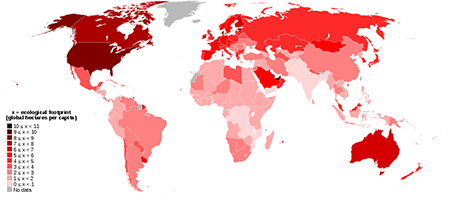
\includegraphics[width=4.6875in,height=2.07292in]{oko_labnyom.png}}

\end{ajanlofig}

The \textbf{ecological footprint} measures human demand on nature, i.e.,
the quantity of nature it takes to support people or an economy. It
tracks this demand through an ecological accounting system. The accounts
contrast the biologically productive area people use for their
consumption to the biologically productive area available within a
region or the world
(\href{https://en.wikipedia.org/wiki/Biocapacity}{biocapacity}). In
short, it is a measure of
\href{https://en.wikipedia.org/wiki/Human_impact_on_the_environment}{human
impact on Earth's ecosystem} and reveals the dependence of the human
economy on \href{https://en.wikipedia.org/wiki/Natural_capital}{natural
capital}.

The ecological footprint is defined as the biologically productive area
needed to provide for everything people use: fruits and vegetables,
fish, wood, fibers, absorption of carbon dioxide from fossil fuel use,
and space for buildings and roads. Biocapacity is the productive area
that can regenerate what people demand from nature.

\end{ajanlo}

\hypertarget{monoton-novekedes-es-fogyas}{%
\subsection{Monoton növekedés és
fogyás}\label{monoton-novekedes-es-fogyas}}

\begin{definicio}

Definíció:\\
Azt mondjuk, hogy az
\(\left. f:{\mathbb{R}}\rightarrow{\mathbb{R}} \right.\) egy \(I\)
intervallumon

\begin{itemize}
\tightlist
\item
  Monoton nő, ha \(\forall x_{1},x_{2} \in I\) esetén
  \(\left. x_{1} < x_{2}\Rightarrow f\left( x_{1} \right) \leq f\left( x_{2} \right) \right.\).
\item
  Monoton csökken, ha \(\forall x_{1},x_{2} \in I\) esetén
  \(\left. x_{1} < x_{2}\Rightarrow f\left( x_{1} \right) \geq f\left( x_{2} \right) \right.\).
\item
  Szigorú monoton nő, ha \(\forall x_{1},x_{2} \in I\) esetén
  \(\left. x_{1} < x_{2}\Rightarrow f\left( x_{1} \right) < f\left( x_{2} \right) \right.\).
\item
  Szigorú monoton csökken, ha \(\forall x_{1},x_{2} \in I\) esetén
  \(\left. x_{1} < x_{2}\Rightarrow f\left( x_{1} \right) > f\left( x_{2} \right) \right.\).
\end{itemize}

\end{definicio}

\begin{tetel}

Tétel (Rolle-tétel):\\
Tfh
\(\left. f:\left\lbrack {a,b} \right\rbrack\rightarrow{\mathbb{R}} \right.\)
folytonos és \(\left( {a,b} \right)\)-n differenciálható,
\(f\left( a \right) = f\left( b \right)\). Ekkor
\(\exists\xi \in \left( {a,b} \right):f'\left( \xi \right) = 0\).

\end{tetel}

\begin{bizonyitas}

Bizonyítás:

\begin{enumerate}
\def\labelenumi{\arabic{enumi}.}
\tightlist
\item
  Ha
  \(f\left( x \right) = f\left( a \right) = f\left( b \right),\forall x\),
  akkor
  \(f'\left( x \right) = 0\quad\forall x \in \left( {a,b} \right)\).
\item
  Ha létezik
  \(x \in \left( {a,b} \right):f\left( x \right) \neq f\left( a \right) = f\left( b \right)\),
  pl \(f\left( x \right) < f\left( a \right)\), akkor mivel
  \(\left. f \in C\left\lbrack {a,b} \right\rbrack\Rightarrow\left\lbrack {a,b} \right\rbrack \right.\)
  sorozatkompakt halmaz \(\mathbb{R}\)-ben (ami korlátos és zárt) ezért
  \(R_{f}\) sorozatkompakt \(\Rightarrow\) korlátos és zárt.
  \(\exists\xi \in \left\lbrack {a,b} \right\rbrack:f\left( \xi \right) = \inf f = \min f\).
  Mivel
  \(\exists f\left( x \right):f\left( x \right) < f\left( a \right)\),
  ezért \(\xi \in \left( {a,b} \right)\). Ezért \(f\)-nek \(\xi\)-ben
  lokális minimuma van. \(f\) differenciálható \(\xi\)-ben, tehát
  \(f'\left( \xi \right) = 0\). ■
\end{enumerate}

\end{bizonyitas}

\begin{tetel}

Tétel (Lagrange-féle középértéktétel):\\
\(\left. f:\left\lbrack {a,b} \right\rbrack\rightarrow{\mathbb{R}},f \in C\left( D_{f} \right) \right.\)
és \(f\) differenciálható \(\left( {a,b} \right)\)-n. Ekkor
\(\exists\xi \in \left( {a,b} \right):f'\left( \xi \right) = \frac{f\left( b \right) - f\left( a \right)}{b - a}\).

\end{tetel}

\begin{bizonyitas}

Bizonyítás:\\
Visszavezetjük a Rolle-tételre. Értelmezzük a \(g\) függvényt a
következő módon:
\(g\left( x \right) = f\left( x \right) - \frac{f\left( b \right) - f\left( a \right)}{b - a}\left( {x - a} \right)\).
Ekkor \(g \in C\left\lbrack {a,b} \right\rbrack\) és \(g\)
differenciálható \(\left( {a,b} \right)\)-n.
\(g\left( b \right) = f\left( b \right) - \frac{f\left( b \right) - f\left( a \right)}{b - a}\left( {b - a} \right) = f\left( a \right)\),
de a definícióból látható, hogy
\(\left. g\left( a \right) = f\left( a \right)\Rightarrow g\left( b \right) = g\left( a \right) \right.\).
Alkalmazzuk Rolle tételét! \(\exists\xi:g'\left( \xi \right) = 0\), azaz
\(0 = g'\left( \xi \right) = f'\left( \xi \right) - \frac{f\left( b \right) - f\left( a \right)}{b - a}\).
■

\end{bizonyitas}

\begin{tetel}

Tétel:\\
Legyen \(I \subset {\mathbb{R}}\) intervallum!
\(\left. f:I\rightarrow{\mathbb{R}},f \in C\left( I \right) \right.\),
továbbá \(f\) differenciálható \({int}I\)-ben. Ekkor \(f\) monoton nő az
\(I\)-n
\(\left. \Leftrightarrow f'\left( x \right) \geq 0\forall x \in {int}I \right.\).

\end{tetel}

\begin{bizonyitas}

Bizonyítás:

\begin{enumerate}
\def\labelenumi{\arabic{enumi}.}
\tightlist
\item
  Ha \(f\) monoton nő
  \(\left. \Rightarrow\forall x \in {int}I \right.\)-re
  \(f'\left( x \right) \geq 0\).
\item
  Tfh \(f'\left( x \right) \geq 0\forall x \in {int}I\). Legyen
  \(x_{1},x_{2} \in I\), \(x_{1} < x_{2}\) ! Azt kellene belátni, hogy
  \(f\left( x_{1} \right) \leq f\left( x_{2} \right)\). Alkalmazzuk a
  Lagrange-féle középértéktételt!
  \(\left. \left\lbrack {x_{1},x_{2}} \right\rbrack \subset I\Rightarrow\exists\xi \in \left( {x_{1},x_{2}} \right) \subset I:f'\left( \xi \right) = \frac{f\left( x_{2} \right) - f\left( x_{1} \right)}{x_{2} - x_{1}} \right.\).
  A feltétel szerint
  \(\left. f'\left( \xi \right) \geq 0,x_{2} - x_{1} > 0\Rightarrow f\left( x_{2} \right) - f\left( x_{1} \right) \geq 0\Rightarrow f\left( x_{2} \right) \geq f\left( x_{1} \right) \right.\).
\end{enumerate}

\end{bizonyitas}

\begin{megjegyzes}

Megjegyzés:\\
Azt hihetnénk, hogy \(f\) szigorúan monoton növekedése
\(\left. \Leftrightarrow f'\left( x \right) > 0\forall x \in {int}D_{f} \right.\),
pedig nem. Példa: \(f\left( x \right) = x^{3},x \in {\mathbb{R}}\).
Ekkor \(f\) szigorúan monoton nő, de \(f'\left( 0 \right) = 0\).

\end{megjegyzes}

\begin{tetel}

Tétel:\\
Legyen \(I \subset {\mathbb{R}}\) intervallum,
\(\left. f:I\rightarrow{\mathbb{R}},f \in C\left( I \right) \right.\) és
\(f\) differenciálható \({int}I\)-ben! Ekkor \(f\) szigorúan monoton nő
\(I\)-n \(\left. \Leftrightarrow f'\left( x \right) \geq 0 \right.\) és
\(I\)-nek nincs olyan \(J\) részintervalluma, ahol
\(f'\left( x_{j} \right) = 0,\forall x_{j} \in J\).

\end{tetel}

\begin{bizonyitas}

Bizonyítás:

\begin{itemize}
\tightlist
\item
  \(\Rightarrow\) irányban: tfh \(f\) szigorúan monoton nő az \(I\)-n
  \(\Rightarrow\) monoton nő
  \[\left. \Rightarrow f'\left( x \right) \geq 0\quad\forall x \in {int}\left( I \right) \right.\].
  Indirekt tfh
  \[\left. \exists\left( {c,d} \right) \subset I:f'\left( x \right) = 0\forall x \in \left( {c,d} \right)\Rightarrow \right.\]
  Lagrange-féle középértéktétel felhasználásából
  \(\left. \Rightarrow f = \text{állandó} \right.\)
  \(\left( {c,d} \right)\) -n. Ez ellentmond annak, hogy \(f\) szigorúan
  monoton nő.
\item
  \(\Leftarrow\) irányban: tfh
  \(f'\left( x \right) \geq 0\forall x \in {int}I\) és
  \(\nexists J \subset I\) részintervallum, ahol
  \(f'\left( x_{j} \right) = 0\forall x_{j} \in J\). Mivel
  \(\left. f'\left( x \right) \geq 0\Rightarrow f \right.\) monoton nő.
  Ha \(f\) nem szigorúan monoton növő lenne, akkor
  \(\left. \exists x_{1},x_{2} \in I,x_{1} < x_{2}:f\left( x_{1} \right) = f\left( x_{2} \right)\Rightarrow \right.\)
  (mivel \(f\) monoton nő)
  \(\left. f\left( x_{1} \right) = f\left( x \right) = f\left( x_{2} \right)\forall x \in \left( {x_{1},x_{2}} \right)\Rightarrow\operatorname{}f'\left( x \right) = 0 \right.\),
  ha \(x \in \left( {x_{1},x_{2}} \right)\). ■
\end{itemize}

\end{bizonyitas}

\begin{tetel}

Tétel:\\
Tfh \(\left. f:{\mathbb{R}}^{n}\rightarrowtail{\mathbb{R}} \right.\), és
ennek az összes elsőrendű parciális deriváltja létezik
\(x_{0} \in {\mathbb{R}}^{n}\) valamely teljes környezetében, és ezek
folytonosak \(x_{0}\)-ban. Ekkor \(f\) differenciálható \(x_{0}\)-ban.

\end{tetel}

\begin{bizonyitas}

Bizonyítás:\\
A feltétel szerint egy \(x_{0}\) bizonyos környezetében fekvő
\(x = \left( {x_{1},x_{2}...x_{n}} \right)\) pontra \[\begin{aligned}
  f\left( x \right) - f\left( {{x_0}} \right) =  & \left[ {f\left( {{x_1},{x_2}...{x_n}} \right) - f\left( {{x_{1,0}},{x_2}...{x_n}} \right)} \right] \\ 
   +  & \left[ {f\left( {{x_{1,0}},{x_2}...{x_n}} \right) - f\left( {{x_{1,0}},{x_{2,0}}...{x_n}} \right)} \right] \\ 
   +  & ... \\ 
   +  & \left[ {f\left( {{x_{1,0}},{x_{2,0}}...{x_{n - 1,0}},{x_n}} \right) - f\left( {{x_{1,0}}...{x_{n,0}}} \right)} \right], \\ 
\end{aligned} \]alkalmasan választott
\(\xi_{i} \in \left( {x_{i},x_{i,0}} \right)\) segítségével folytatva
(Lagrange-féle középértéktétel felhasználásával): \[\begin{aligned}
  f\left( x \right) - f\left( {{x_0}} \right) =  & {\partial _1}f\left( {{\xi _1},{x_2}...{x_n}} \right)\left( {{x_1} - {x_{1,0}}} \right) \\ 
   &  + {\partial _2}f\left( {{x_{1,0}},{\xi _2},{x_3}...{x_n}} \right)\left( {{x_2} - {x_{2,0}}} \right) \\ 
   &  + ... \\ 
   &  + {\partial _n}f\left( {{x_{1,0}},{x_{2,0}}...{x_{n - 1,0}},{\xi _n}} \right)\left( {{x_n} - {x_{n,0}}} \right) \\ 
   =  & {\partial _1}f\left( {{x_0}} \right)\left( {{x_1} - {x_{1,0}}} \right) \\ 
   &  + {\partial _2}f\left( {{x_0}} \right)\left( {{x_2} - {x_{2,0}}} \right) \\ 
   &  + ... \\ 
   &  + {\partial _n}f\left( {{x_0}} \right)\left( {{x_n} - {x_{n,0}}} \right) \\ 
   &  + \underbrace {\left[ {{\partial _1}f\left( {{\xi _1},{x_2}...{x_n}} \right) - {\partial _1}f\left( {{x_0}} \right)} \right]\left( {{x_1} - {x_{1,0}}} \right)}_{{\eta _1}\left( x \right)} \\ 
   &  + \underbrace {\left[ {{\partial _2}f\left( {{x_{1,0}},{\xi _2},{x_3}...{x_n}} \right) - {\partial _2}f\left( {{x_0}} \right)} \right]\left( {{x_2} - {x_{2,0}}} \right)}_{{\eta _2}\left( x \right)} \\ 
   &  + ... \\ 
   &  + \underbrace {\left[ {{\partial _n}f\left( {{x_{1,0}},{x_{2,0}},...,{x_{n - 1,0}}{\xi _n}} \right) - {\partial _n}f\left( {{x_0}} \right)} \right]\left( {{x_n} - {x_{n,0}}} \right)}_{{\eta _3}\left( x \right)}. \\ 
\end{aligned} \] Azt kellene belátni, hogy
\(\underset{x\rightarrow x_{0}}{\lim}\frac{\eta\left( x \right)}{\left| {x - x_{0}} \right|} = 0\)
ahol
\(\eta\left( x \right) = {\sum\limits_{i = 1}^{n}{\eta_{i}\left( x \right)}}\).
Hasonló egyenlőség érvényes \(\eta\left( x \right)\) minden tagjára, pl.
az 1-re az alábbi.
\[\frac{{\left| {\left[ {{\partial _1}f\left( {{\xi _1},{x_2}...{x_n}} \right) - {\partial _1}f\left( {{x_0}} \right)} \right]\left( {{x_1} - {x_{1,0}}} \right)} \right|}}{{\left| {x - {x_0}} \right|}} \leqslant \underbrace {\left[ {{\partial _1}f\left( {{\xi _1},{x_2}...{x_n}} \right) - {\partial _1}f\left( {{x_0}} \right)} \right]}_{x \to {x_0}{\text{\;\'e s\;}}{\partial _1}f \in C\left( {{x_0}} \right) \Rightarrow {\text{\;ez\;}} \to 0}\underbrace {\frac{{\left| {{x_1} - {x_{1,0}}} \right|}}{{\left| {x - {x_0}} \right|}}}_{ \leqslant 1}\]
■

\end{bizonyitas}

\begin{megjegyzes}

Megjegyzés:\\
A tétel feltétele elegendő, de nem szükséges \(f\)
differenciálhatóságához.

\end{megjegyzes}

\begin{tetel}

Tétel:\\
Legyen
\(\left. f:{\mathbb{R}}^{n}\rightarrowtail{\mathbb{R}}^{m}\left( {m > 1} \right) \right.\).
\(f = \left( {f_{1},f_{2}...f_{n}} \right)\). Az, hogy \(f\)
differenciálható \(x_{0}\)-ben
\(\left. \Leftrightarrow\forall j \right.\)-re \(f_{j}\)
differenciálható \(x_{0}\)-ban,
\(\left. f_{j}:{\mathbb{R}}^{n}\rightarrowtail{\mathbb{R}} \right.\).

\end{tetel}

Következmény: ha \(\partial_{k}f_{j}\) létezik \(x_{0}\) egy
környezetében és folytonos \(x_{0}\)-ban \(\forall j,k\)-ra, akkor \(f\)
differenciálható \(x_{0}\)-ban.

\begin{bizonyitas}

Bizonyítás:\\
\(f\) differenciálható \(x_{0}\)-ban
\(\left. \Rightarrow f\left( x \right) - f\left( x_{0} \right) = \mathcal{A}\left( {x - x_{0}} \right) + \eta\left( x \right) \right.\)
ahol
\(\underset{x\rightarrow x_{0}}{\lim}\frac{\eta\left( x \right)}{\left| {x - x_{0}} \right|} = 0,\quad\eta = \left( {\eta_{1},\eta_{2},\eta_{3}...\eta_{n}} \right)\).
„Koordinátás" alakban így is írhattuk volna:
\(f_{j}\left( x \right) - f_{j}\left( x_{0} \right) = \mathcal{A}_{j}\left( {x - x_{0}} \right) + \eta_{j}\left( x \right)\)
\(\forall j\)-re, ahol \[{\mathcal{A} = \left( \begin{array}{llll}
a_{11} & a_{12} & \cdots & a_{1n} \\
a_{21} & a_{22} & \cdots & a_{2n} \\
 \vdots & \vdots & \ddots & \vdots \\
a_{m1} & a_{m2} & \cdots & a_{mn} \\
\end{array} \right)}.\] illetve
\(\mathcal{A}_{k} = \left( {a_{k1},a_{k2}...a_{kn}} \right)\). Ez
pontosan azt jelenti, hogy \(f_{j}\) koordinátafüggvény differenciálható
\(x_{0}\) -ban. ■

\end{bizonyitas}

\begin{definicio}

Definíció:\\
Legyen \(X\), \(Y\) normált terek,
\(\left. f:X\rightarrowtail Y,\Omega \subset X \right.\) tartomány
(vagyis nyílt és összefüggő). Ha az \(f\) az \(\Omega\) minden pontjában
differenciálható, akkor azt mondjuk, hogy \(f\) differenciálható
\(\Omega\)-n.

\end{definicio}

\begin{definicio}

Definíció:\\
Legyen
\(\left. f:{\mathbb{R}}^{n}\rightarrowtail{\mathbb{R}},\Omega \subset {\mathbb{R}} \right.\)
! Ha \(\forall j\)-re
\(\exists\partial_{j}f\left( x \right),\forall x \in \Omega\), akkor
\(f\) egyszer parciálisan differenciálható \(\Omega\)-ban. Ha
\(\partial_{j}f\) folytonos is \(\Omega\) minden pontjában
\(\forall j\)-re, akkor \(f\) egyszer folytonosan differenciálható
\(\Omega\)-n, \(f' \in C\left( \Omega \right)\).

\end{definicio}

\hypertarget{magasabbrendu-differencialhatosag}{%
\subsection{Magasabbrendű
differenciálhatóság}\label{magasabbrendu-differencialhatosag}}

\begin{definicio}

Definíció:\\
Legyenek \(X\), \(Y\) normált terek,
\(\left. f:X\rightarrowtail Y \right.\). Tekintsük az összes \(x \in X\)
pontot, melyben \(f\) differenciálható! Azt a függvényt, amely az ilyen
\(x \in X\) ponthoz az \(f'\left( x \right) \in L\left( {X,Y} \right)\)
deriváltat rendeli, \(f\) (első) derivált függvényének nevezzük, jele
\(f'\).

\end{definicio}

\begin{definicio}

Definíció:\\
Legyenek \(X\), \(Y\) normált terek,
\(\left. f:X\rightarrowtail Y \right.\). Ha \(f'\) differenciálható
\(x_{0}\)-ban (tehát értelmezve is van \(x_{0}\) egy környezetében),
akkor azt mondjuk, hogy \(f\) kétszer differenciálható \(x_{0}\)-ban és
definíció szerint
\(f''\left( x_{0} \right): = \left( {f'} \right)'\left( x_{0} \right)\).\\
Megjegyzés:
\(\left. f''\left( x_{0} \right):X\rightarrowtail L\left( {X,Y} \right) \right.\),
\(f''\left( x_{0} \right)\) lineáris folytonos operátor, így
\(f''\left( x_{0} \right) \in L\left( {X,L\left( {X,Y} \right)} \right)\).

\end{definicio}

\begin{definicio}

Definíció:\\
Ha \(f'\) függvény értelmezve van és folytonos valamely
\(\Omega \subset X\) tartományon, akkor azt mondjuk, hogy \(f\) egyszer
folytonosan differenciálható \(\Omega\)-n.

\end{definicio}

\begin{megjegyzes}

Megjegyzés:\\
Gyakran beszélünk \(\overline{\Omega}\)-beli folytonos deriválhatóságról
is. Ez akkor teljesül, ha \(f^{\prime}\) folytonosan kierjeszthető
\(\Omega\)-ról az \(\overline{\Omega}\) halmazra.

\end{megjegyzes}

\begin{megjegyzes}

Megjegyzés:\\
Ez a definíció \(X = {\mathbb{R}}^{n},Y = {\mathbb{R}}\) esetén
ekvivalens a korábbi definícióval.

\end{megjegyzes}

\begin{definicio}

Definíció:\\
Ha \(f\) ' függvény értelmezve van és folytonos valamely
\(\Omega \subset X\) tartományon, akkor azt mondjuk, hogy \(f\) kétszer
folytonosan differenciálható \(\Omega\)-n.

\end{definicio}

\begin{definicio}

Definíció:\\
Legyen \(\left. f:{\mathbb{R}}^{n}\rightarrowtail{\mathbb{R}} \right.\)
képező függvény! Ha valamely \(j\)-re a \(\partial_{j}f\) függvény a
\(k\)-adik változója szerint parciálisan differenciálható egy
\(x_{0} \in {\mathbb{R}}^{n}\) pontjában, akkor
\(\partial_{k}\partial_{j}f\left( x_{0} \right): = \left\lbrack {\partial_{k}\left( {\partial_{j}f} \right)} \right\rbrack x_{0}\).
Hasonlóan értelmezhető \(f\) függvény magasabb rendű parciális
deriváltjaira.

\end{definicio}

Kérdés: igaz-e, hogy
\(\partial_{j}\partial_{k}f = \partial_{k}\partial_{j}f\),
\(\forall j,k\) -ra? Általában nem (de azért a fizikában előforduló
példákra általában igaz, mint ahogy látni is fogjuk). Példa az alábbi.
\[f\left( {x,y} \right): = \begin{cases}
\frac{xy^{3}}{\left( {x^{2} + y^{2}} \right)} & {\text{ha~}\left( {x,y} \right) \neq \left( 0,0 \right)} \\
0 & {\text{ha~}\left( {x,y} \right) = \left( 0,0 \right)} \\
\end{cases}\] Ekkor \(\partial_{1}\partial_{2}f\left( 0,0 \right) = 0\),
de \(\partial_{2}\partial_{1}f\left( 0,0 \right) = 1\) . Az eredmények
nem triviálisak, segítségképp az egyes parciális deriváltak alant.
\[\partial_{1}f\left( {x,y} \right) = \begin{cases}
\frac{y^{5} - x^{2}y^{3}}{\left( {x^{2} + y^{2}} \right)^{2}} & {\text{ha~}\left( {x,y} \right) \neq \left( 0,0 \right)} \\
0 & {\text{ha~}\left( {x,y} \right) = \left( 0,0 \right)} \\
\end{cases}\] \[\partial_{2}f\left( {x,y} \right) = \begin{cases}
\frac{3x^{3}y^{2} + xy^{2}}{\left( {x^{2} + y^{2}} \right)^{2}} & {\text{ha~}\left( {x,y} \right) \neq \left( 0,0 \right)} \\
0 & {\text{ha~}\left( {x,y} \right) = \left( 0,0 \right)} \\
\end{cases}\]

\begin{tetel}

Tétel (Young-tétel) :\\
\({\mathbb{R}}^{2}\)-ből \(\mathbb{R}\)-be képező függvényekre: legyen
\(\left. f:{\mathbb{R}}^{2}\rightarrowtail{\mathbb{R}} \right.\), melyre
\(\left( {x_{0},y_{0}} \right) \in D_{f} \subset {\mathbb{R}}^{2}\) pont
környezetében létezik \(\partial_{1}\partial_{2}f\) és
\(\partial_{2}\partial_{1}f\) is és folytonosak
\(\left( {x_{0},y_{0}} \right)\) pontban. Ekkor
\(\partial_{1}\partial_{2}f\left( {x_{0},y_{0}} \right) = \partial_{2}\partial_{1}f\left( {x_{0},y_{0}} \right)\).

\end{tetel}

\begin{bizonyitas}

Bizonyítás: \[\left. \left. \begin{array}{l}
{F\left( x \right): = f\left( {x,y} \right) - f\left( {x,y_{0}} \right)} \\
{G\left( y \right): = f\left( {x,y} \right) - f\left( {x_{0},y} \right)} \\
\end{array} \right\}\Rightarrow F\left( x \right) - F\left( x_{0} \right) = G\left( y \right) - G{\left( y_{0} \right).} \right.\]
Alkalmazzuk először a Lagrange-féle középértéktételt \(F\) és \(G\)
függvényekre! \(\exists\xi\) az \(x,x_{0}\) között, hogy
\[F\left( x \right) - F\left( x_{0} \right) = F'\left( \xi \right)\left( {x - x_{0}} \right) = \left\lbrack {\partial_{1}f\left( {\xi,y} \right) - \partial_{1}f\left( {\xi,y_{0}} \right)} \right\rbrack{\left( {x - x_{0}} \right),}\]
és \(\exists\eta\) az \(y,y_{0}\) között, hogy
\[G\left( y \right) - G\left( y_{0} \right) = G'\left( \eta \right)\left( {y - y_{0}} \right) = \left\lbrack {\partial_{2}f\left( {x,\eta} \right) - \partial_{2}f\left( {x_{0},\eta} \right)} \right\rbrack{\left( {y - y_{0}} \right),}\]
ezért a fenti egyenlőség miatt
\[\left\lbrack {\partial_{1}f\left( {\xi,y} \right) - \partial_{1}f\left( {\xi,y_{0}} \right)} \right\rbrack\left( {x - x_{0}} \right) = \left\lbrack {\partial_{2}f\left( {x,\eta} \right) - \partial_{2}f\left( {x_{0},\eta} \right)} \right\rbrack{\left( {y - y_{0}} \right).}\]
Még 2x alkalmazzuk a Lagrange-féle középértéktételt:
\(\left. y\mapsto\partial_{1}f\left( {\xi,y} \right) \right.\)
függvényre és
\(\left. x\mapsto\partial_{2}f\left( {x,\eta} \right) \right.\)
függvényre.
\[\exists\widetilde{\xi},\widetilde{\eta}:\partial_{2}\left( {\partial_{1}f} \right)\left( {\xi,\widetilde{\eta}} \right)\left( {y - y_{0}} \right)\left( {x - x_{0}} \right) = \partial_{1}\left( {\partial_{2}f} \right)\left( {\widetilde{\xi},\eta} \right)\left( {x - x_{0}} \right){\left( {y - y_{0}} \right),}\]
ahol \(\widetilde{\xi}\) egy \(x,x_{0}\) között, \(\widetilde{\eta}\)
pedig egy \(y,y_{0}\) között van.
\(\partial_{2}\left( {\partial_{1}f} \right)\left( {\xi,\widetilde{\eta}} \right) = \partial_{1}\left( {\partial_{2}f} \right)\left( {\widetilde{\xi},\eta} \right)\).
\(\left. \left( {x,y} \right)\rightarrow\left( {x_{0},y_{0}} \right) \right.\)
esetén, mivel \(\partial_{1}\partial_{2}f\) és
\(\partial_{2}\partial_{1}f\) folytonosak
\(\left( {x_{0},y_{0}} \right)\)-ban,
\(\left. \Rightarrow\partial_{2}\left( {\partial_{1}f} \right)\left( {x_{0},y_{0}} \right) = \partial_{1}\left( {\partial_{2}f} \right)\left( {x_{0},y_{0}} \right) \right.\).
■

\end{bizonyitas}

Következmény: ha
\(\left. f:{\mathbb{R}}^{n}\rightarrow{\mathbb{R}} \right.\)-be képez és
az \(f\)-nek az összes második parciális deriváltja létezik \(x_{0}\)
egy környezetében és folytonos \(x_{0}\)-ban
\(\left. \Rightarrow\partial_{j}\partial_{k}f\left( x_{0} \right) = \partial_{k}\partial_{j}f\left( x_{0} \right) \right.\).

\begin{ajanlo}

\begin{ajanlofig}

\href{https://www.youtube.com/watch?v=ye27aIJD6qg}{
\includegraphics[width=4.6875in,height=3.25in]{mrbean.jpg}}

\end{ajanlofig}

Ebből a tárgyból egyesek jó eredményt értek el, mások megbuktak. A siker
kulcsa lehet, hogy időben állsz neki tanulni. Ha stresszeled magad,
akkor a tanulás nehezebbé válhat, ezért fontos időben hozzálátni. A
vizsgára 3 napi tanulás (3x12 óra) nem túlzás, a legkevésbé sem.

\end{ajanlo}

\begin{definicio}

Definíció:\\
Azt mondjuk, hogy egy
\(\left. f:{\mathbb{R}}^{n}\rightarrow{\mathbb{R}} \right.\) függvény
\(k\)-szor (\(k \geq 1\)) folytonosan differenciálható \(\Omega\)-n, ha
minden legfeljebb \(k\)-ad rendű parciális derivált létezik és folytonos
az \(\Omega \subset {\mathbb{R}}^{n}\) tartományon.

\end{definicio}

\begin{tetel}

Tétel:\\
Ha \(\left. f:\Omega\rightarrow{\mathbb{R}} \right.\) függvény
\(k\)-szor folytonosan differenciálható, akkor \(f\) minden legfeljebb
\(k\)-adrendű parciális deriváltjában a deriválások sorrendje
tetszőlegesen felcserélhető.

\end{tetel}

Jelölés: feltéve, hogy \(f\) függvény \(k\)-szor folytonosan
differenciálható, a továbbiakban használandó a következő jelölés a
legfeljebb \(k\)-adrendű parciális deriváltakra:
\(\alpha = \left( {\alpha_{1},\alpha_{2}...\alpha_{n}} \right),\alpha_{j} \geq 0,\alpha_{j} \in {\mathbb{N}}\)
esetén
\(\partial^{\alpha}f: = \partial_{1}^{\alpha_{1}}\partial_{2}^{\alpha_{2}}...\partial_{n}^{\alpha_{n}}f\).
A deriválás rendje
\(\left| \alpha \right| = {\sum\limits_{j = 1}^{n}\alpha_{j}} \leq k\).

\begin{megjegyzes}

Megjegyzés:\\
Ha \(\left. f:{\mathbb{R}}^{n}\rightarrowtail{\mathbb{R}} \right.\)
függvény \(k\)-szor folytonosan differenciálható
\(\left. \Omega\text{-n}\Rightarrow f \right.\) minden legfeljebb
\(\left( {k - 1} \right)\)-edrendű parciális deriváltja
differenciálható.

\end{megjegyzes}

\hypertarget{bilinearis-operatorok}{%
\subsection{Bilineáris operátorok}\label{bilinearis-operatorok}}

Azért kellenek, mert
\(f''\left( x_{0} \right) \in L\left( {X,L\left( {X,Y} \right)} \right)\),
és ezt összefüggésbe akarjuk hozni az \(X\) × \(X\)-ből \(Y\)-ba képező
operátorokkal.

\begin{definicio}

Definíció:\\
Legyenek \(X\), \(Y\) vektorterek, ekkor
\(X \times Y:\left\{ \left( {x,y} \right) \middle| x \in X,y \in Y \right\}\)
és \(X\) × \(Y\)-n értelmezzük az összeadást és a valós számmal való
szorzást:
\(\left( {x_{1},y_{1}} \right) + \left( {x_{2},y_{2}} \right) = \left( {x_{1} + x_{2},y_{1} + y_{2}} \right)\),
\(\lambda \in {\mathbb{R}}\) esetén
\(\lambda\left( {x_{1},y_{1}} \right) = \left( {\lambda x_{1},\lambda y_{1}} \right)\).

\end{definicio}

\begin{allitas}

Állítás:\\
az \(X\) × \(Y\) a fenti tulajdonságokkal vektorteret alkot.

\end{allitas}

\begin{definicio}

Definíció:\\
Legyenek \(X\), \(Y\) normált terek. Ekkor az \(X \times Y\)
vektortérben vezessük be a következő normát:
\(\left\| \left( {x,y} \right) \right\|: = \sqrt{\left\| x \right\|^{2} + \left\| y \right\|^{2}}\)
!\\
(Megj: más normát is lehetne definiálni, pl
\(\left\| {x,y} \right\|: = \left\| x \right\| + \left\| y \right\|\)).

\end{definicio}

\begin{allitas}

Állítás:\\
\(X\) × \(Y\) a fenti normával normált tér.

\end{allitas}

\begin{definicio}

Definíció:\\
Legyenek \(X\), \(Y\), \(Z\) normált terek, tekintsük az \(X \times Y\)
vektorteret! Egy
\(\left. \widetilde{A}:X \times Y\rightarrow Z \right.\) operátort
bilineárisnak nevezünk, ha minden rögzített \(\forall x \in X\) esetén
az \(\left. y\mapsto\widetilde{A}\left( {x,y} \right) \right.\)
hozzárendeléssel adott\(\left. Y\rightarrow Z \right.\) lineáris és
minden rögzített \(y \in Y\) esetén az
\(\left. x\mapsto\widetilde{A}\left( {x,y} \right) \right.\)
hozzárendeléssel adott \(\left. Y\rightarrow Z \right.\) operátor
lineáris.

\end{definicio}

\begin{megjegyzes}

Megjegyzés:\\
Az \(X\) × \(Y\)-ből \(Z\)-be képező bilineáris operátorok vektorteret
alkotnak a következő művelettel:
\(\underbrace {\left( {\tilde A + \tilde B} \right)}_{ \in L\left( {X \times Y,Z} \right)}\underbrace {\left( {x,y} \right)}_{ \in X \times Y} = \underbrace {\tilde A\left( {x,y} \right)}_{ \in Z} + \underbrace {\tilde B\left( {x,y} \right)}_{ \in Z},\)
és \(\lambda \in {\mathbb{R}}\) esetén
\(\left( {\lambda\widetilde{A}} \right)\left( {x,y} \right) = \lambda \cdot \widetilde{A}\left( {x,y} \right) \in Z\).

\end{megjegyzes}

Kérdés: legyenek \(X\), \(Y\), \(Z\) normált terek (tehát vektorterek
is). Továbbá legyen
\(\left. \widetilde{A}:X \times Y\rightarrow Z \right.\) bilineáris
operátor. Következik-e ebből, hogy \(\widetilde{A}\) folytonos?
Általában nem.

\begin{tetel}

Tétel:\\
Az \(\left. \widetilde{A}:X \times Y\rightarrowtail Z \right.\)
bilineáris operátor pontosan akkor folytonos, ha
\(\exists c \geq 0:\left\| {\widetilde{A}\left( {x,y} \right)} \right\| \leq c\left\| x \right\| \cdot \left\| y \right\|\),
\(\forall x \in X,\forall y \in Y.\)

\end{tetel}

\begin{megjegyzes}

Megjegyzés:\\
Ha az utóbbi teljesül, akkor \(\widetilde{A}\) bilineáris operátort
korlátosnak nevezzük.

\end{megjegyzes}

\begin{bizonyitas}

Bizonyítás:

\begin{itemize}
\tightlist
\item
  \(\Leftarrow\) irányban: tfh \(\widetilde{A}\) korlátos. Belátjuk,
  hogy \(\widetilde{A}\) folytonos
  \(\left( {x_{0},y_{0}} \right) \in X \times Y\) rögzített elemnél,
  ekkor \[\begin{aligned}
    \left\| {\tilde A\left( {x,y} \right) - \tilde A\left( {{x_0},{y_0}} \right)} \right\| =  & \left\| {\left[ {\tilde A\left( {x,y} \right) - \tilde A\left( {{x_0},y} \right)} \right] + \left[ {\tilde A\left( {{x_0},y} \right) - \tilde A\left( {{x_0},{y_0}} \right)} \right]} \right\| \\ 
     \leqslant  & \left\| {\left[ {\tilde A\left( {x,y} \right) - \tilde A\left( {{x_0},y} \right)} \right] + \left[ {\tilde A\left( {{x_0},y} \right) - \tilde A\left( {{x_0},{y_0}} \right)} \right]} \right\| \\ 
     \leqslant  & \left\| {\tilde A\left( {x - {x_0},y} \right)} \right\| + \left\| {\tilde A\left( {{x_0},y - {y_0}} \right)} \right\| \\ 
     \leqslant  & c\left\| {x - {x_0}} \right\| \cdot \left\| y \right\| + c\left\| {{x_0}} \right\| \cdot \left\| {y - {y_0}} \right\|, \\ 
  \end{aligned} \] ezért nyílván
  \[\forall \varepsilon  > 0\exists \delta  > 0:\left\| {\left( {x,y} \right) - \left( {{x_0},{y_0}} \right)} \right\| = \sqrt {{{\left\| {x - {x_0}} \right\|}^2} + {{\left\| {y - {y_0}} \right\|}^2}}  < \delta, \]
  amelyből következik, hogy
  \[c\left\| {x - {x_0}} \right\| \cdot \left\| y \right\| + c\left\| {{x_0}} \right\| \cdot \left\| {y - {y_0}} \right\| < \varepsilon .\]
\item
  \(\Rightarrow\) irányban: tfh folytonos, de nem korlátos (indirekt):
  \(\forall n \in {\mathbb{N}}\exists x_{n} \in X,y_{n} \in Y:\left\| {\widetilde{A}\left( {x_{n},y_{n}} \right)} \right\| > n^{2}\left\| x_{n} \right\| \cdot \left\| y_{n} \right\|\).
  Legyen
  \(\left. \widetilde{x_{n}}: = \frac{x_{n}}{n \cdot \left\| x_{n} \right\|}\rightarrow 0 \right.\)
  és
  \(\left. \widetilde{y_{n}}: = \frac{y_{n}}{n \cdot \left\| y_{n} \right\|}\rightarrow 0 \right.\).
  Ebből már látszik az állítás. ■
\end{itemize}

\end{bizonyitas}

\begin{definicio}

Definíció:\\
Legyenek \(X\), \(Y\), \(Z\) normált terek,
\(\left. \widetilde{A}:X \times Y\rightarrowtail Z \right.\) korlátos,
folytonos bilineáris operátor. Ekkor \(\widetilde{A}\) normáját így
értelmezzük:
\[\left\| \widetilde{A} \right\|: = \sup{\left\{ {\left\| {\widetilde{A}\left( {x,y} \right)} \right\|:\left\| x \right\| = 1,\left\| y \right\| = 1} \right\}.}\]

\end{definicio}

\begin{allitas}

Állítás:\\
\(\left\| \widetilde{A} \right\| = \min\left\{ {c:\left\| {\widetilde{A}\left( {x,y} \right)} \right\| \leq c\left\| x \right\| \cdot \left\| y \right\|,\forall\left( {x,y} \right) \in X \times Y} \right\}\).
(A bizonyítása hasonló lineáris korlátos operátorok esetéhez.)

\end{allitas}

\begin{tetel}

Tétel:\\
Tekintsük az \(\left. X \times Y\rightarrow Z \right.\) képező korlátos
bilineáris operátorokat az előbb bevezetett összeadással és skalárral
való szorzással, és vegyük hozzá a fenti normát. Ekkor egy normált teret
kapunk.

\end{tetel}

Észrevétel: legyenek \(X\), \(Y\), \(Z\) normált terek,
\(A \in L\left( {X,L\left( {Y,Z} \right)} \right)\). Értelmezzük az
\(\left. \widetilde{A}:X \times Y\rightarrow Z \right.\) operátort:
\(\tilde A\left( {x,y} \right): = \underbrace {\left( {Ax} \right)y}_{ \in Z}\).
Ekkor \(\left. \widetilde{A}:X \times Y\rightarrow Z \right.\) korlátos
bilineáris operátor.

\begin{bizonyitas}

Bizonyítás:

\begin{enumerate}
\def\labelenumi{\arabic{enumi}.}
\tightlist
\item
  A fentiek szerint
  \(\left. \widetilde{A}:X \times Y\rightarrow Z \right.\).
\item
  Belátjuk először, hogy \(\widetilde{A}\) bilineáris operátor.
  \[\begin{aligned}
    \tilde A\left( {{\lambda _1}{x_1} + {\lambda _2}{x_2},y} \right) =  & \left[ {A\left( {{\lambda _1}{x_1} + {\lambda _2}{x_2}} \right)} \right]y \\ 
     =  & \left( {{\lambda _1}A{x_1} + {\lambda _2}A{x_2}} \right)y \\ 
     =  & {\lambda _1}\left[ {\left( {A{x_1}} \right)y} \right] + {\lambda _2}\left[ {\left( {A{x_2}} \right)y} \right] \\ 
     =  & {\lambda _1}\tilde A\left( {{x_1},y} \right) + {\lambda _2}\tilde A\left( {{x_2},y} \right) \\ 
  \end{aligned} \] \[\begin{aligned}
    \tilde A\left( {x,{\lambda _1}{y_1} + {\lambda _2}{y_2}} \right) &  = \left( {Ax} \right)\left( {{\lambda _1}{y_1} + {\lambda _2}{y_2}} \right) \\ 
     &  = {\lambda _1}\left( {Ax} \right){y_1} + {\lambda _2}\left( {Ax} \right){y_2} \\ 
     &  = {\lambda _1}\tilde A\left( {x,{y_1}} \right) + {\lambda _2}\tilde A\left( {x,{y_2}} \right) \\ 
  \end{aligned} \]
\item
  Belátjuk, hogy \(\widetilde{A}\) korlátos.
  \[\left\| {\tilde A\left( {x,y} \right)} \right\| = \left\| {\left( {Ax} \right)y} \right\| \leqslant \left\| {Ax} \right\| \cdot \left\| y \right\| \leqslant \left\| A \right\| \cdot \left\| x \right\| \cdot \left\| y \right\|,\]
  következésképp \({\tilde A}\) korlátos, továbbá
  \(\left\| \widetilde{A} \right\| \leq \left\| A \right\|\).
\end{enumerate}

\end{bizonyitas}

\begin{tetel}

Tétel:\\
Legyenek \(X\), \(Y\), \(Z\) normált terek,
\(A \in L\left( {X,L\left( {Y,Z} \right)} \right)\). Ekkor az
\(\widetilde{A}\left( {x,y} \right): = \left( {Ax} \right)y,x \in X,y \in Y\)
képlettel értelmezett
\(\left. \widetilde{A}:X \times Y\rightarrow Z \right.\) bilineáris
operátor. Fordítva: minden
\(\left. \widetilde{A}:X \times Y\rightarrow Z \right.\) bilineáris
operátort ilyen alakú:
\(\exists!A:L\left( {X,L\left( {Y,Z} \right)} \right):\widetilde{A}\left( {x,y} \right) = \left( {Ax} \right)y\).

\end{tetel}

\begin{bizonyitas}

Bizonyítás:\\
Az első állítást beláttuk. Fordítva: tfh
\(\left. \widetilde{A}:X \times Y\rightarrow Z \right.\) korlátos
bilineáris operátor. Tekintsük tetszőleges, rögzített \(x \in X\) esetén
a következő \(A\left( x \right)\) operátort:
\(\left. y\mapsto\widetilde{A}\left( {x,y} \right) \right.\). Ez
egyrészt lineáris, másrészt korlátos, hiszen a feltétel szerint
\(\widetilde{A}\) korlátos: \[\begin{aligned}
  \left\| {\left[ {A\left( x \right)} \right]\left( y \right)} \right\| =  & \left\| {\tilde A\left( {x,y} \right)} \right\| \\ 
   =  & \left\| {\tilde A\left( {\frac{x}{{\left\| x \right\|}},\frac{y}{{\left\| y \right\|}}} \right) \cdot \left\| x \right\| \cdot \left\| y \right\|} \right\| \\ 
   \leqslant  & \left\| {\tilde A} \right\| \cdot \left\| x \right\| \cdot \left\| y \right\| \\ 
   =  & \left( {\left\| {\tilde A} \right\| \cdot \left\| x \right\|} \right) \cdot \left\| y \right\|, \\ 
\end{aligned} \] ebből pedig következik, hogy a fenti operátor korlátos
operátor és normája
\(\leq \left\| \widetilde{A} \right\| \cdot \left\| x \right\|\).
Jelölje \(A\left( x \right)\) ezt az \(L\left( {Y,Z} \right)\)-beli
operátort
\(\left. \Rightarrow\widetilde{A}\left( {x,y} \right) = \left( {A\left( x \right)} \right)y \right.\).
Nem nehéz belátni, hogy \(A\left( x \right)\) \(x\)-től lineárisan függ.
\(A\) korlátos is, hisz
\(\left. \left\| {A\left( x \right)} \right\| \leq \left\| \widetilde{A} \right\| \cdot \left\| x \right\|,\forall x \in X\Rightarrow A \right.\)
korlátos is, sőt
\[\left. \left\| A \right\| \leq \left\| \widetilde{A} \right\|\Rightarrow\left\| \widetilde{A} \right\| = \left\| A \right\|. \right.\]
(Lásd az előbbi tételt.) ■

\end{bizonyitas}

\begin{megjegyzes}

Megjegyzés:\\
\(\widetilde{A}\left( {x,y} \right) = \left( {Ax} \right)y\) képlet
lineáris normatartó leképezést definiál a bilineáris operátorok és
\(L\left( {X,L\left( {Y,Z} \right)} \right)\) között.

\end{megjegyzes}

\hypertarget{multilinearis-lekepezesek}{%
\subsection{Multilineáris leképezések}\label{multilinearis-lekepezesek}}

\begin{definicio}

Definíció:\\
Legyenek \(X_{1},X_{2}...X_{n},Z\) vektorterek. Egy
\(\left. X_{1} \times X_{2} \times ... \times X_{n}\rightarrow Z \right.\)
leképezést multilineárisnak nevezünk, ha minden koordinátájában lineáris
(midőn a többit rögzítjük).

\end{definicio}

\begin{definicio}

Definíció:\\
Legyenek \(X_{1},X_{2}...X_{n},Z\) normált terek! Egy
\(\left. \widetilde{A}:X_{1} \times X_{2} \times ... \times X_{n}\rightarrow Z \right.\)
multilineáris leképezés korlátos
\(\exists c \geq 0:\left\| {\widetilde{A}\left( {x_{1},x_{2},...,x_{n}} \right)} \right\| \leq c \cdot \left\| x_{1} \right\| \cdot \left\| x_{2} \right\| \cdot ... \cdot \left\| x_{n} \right\|\forall x_{j} \in X_{j}\).

\end{definicio}

\begin{tetel}

Tétel:\\
\(\widetilde{A}\) folytonos
\(\left. \Leftrightarrow\widetilde{A} \right.\) korlátos.

\end{tetel}

\begin{tetel}

Tétel:\\
Egy \(\widetilde{A}\) multilineáris folytonos operátor általános alakja
\(\widetilde{A}\left( {x_{1},x_{2},x_{3}...x_{n}} \right) = \left( {\left( {\left( {Ax_{1}} \right)x_{2}} \right)x_{3}...x_{n}} \right),A \in L\left( {X_{1},L\left( {X_{2}...L\left( {X_{n},Z} \right)} \right)} \right)\).

\end{tetel}

\hypertarget{alkalmazas-a-magasabbrendu-derivaltak-ertelmezesere}{%
\subsubsection{Alkalmazás a magasabbrendű deriváltak
értelmezésére}\label{alkalmazas-a-magasabbrendu-derivaltak-ertelmezesere}}

Legyenek \(X\), \(Y\) normált terek,
\(\left. f:X\rightarrowtail Y \right.\). Ha \(f\) differenciálható
\(x_{0} \in X\)-ben, akkor
\(f'\left( x_{0} \right) \in L\left( {X,Y} \right)\). \(f'\) függvény
\(X\)-ből \(L\left( {X,Y} \right)\)-ba képező függvény. Ezért
\(f''\left( x_{0} \right) = \left( {f'} \right)'\left( x_{0} \right) \in L\left( {X,L\left( {X,Y} \right)} \right)\).
Az
\(f''\left( x_{0} \right) \in L\left( {X,L\left( {X,Y} \right)} \right)\)-beli
operátornak a fentiek szerint egyértelmű módon megfelel egy
\(\left. X \times X\rightarrow Y \right.\) bilineáris folytonos
operátor: \[\begin{aligned}
  A: =  & f''\left( a \right) \in L\left( {X,L\left( {X,Y} \right)} \right) \\ 
  \tilde A\left( {{x_1},{x_2}} \right): =  & \left( {A{x_1}} \right){x_2} = \left( {\left( {f''\left( a \right)} \right){x_1}} \right){x_2}, \\ 
\end{aligned} \] ahol \(\left( {x_{1},x_{2}} \right) \in X \times X\).

Speciális eset: \(X: = {\mathbb{R}}^{n},Y: = {\mathbb{R}}\). Ekkor
\(\left. f:{\mathbb{R}}^{n}\rightarrow{\mathbb{R}} \right.\),
\[\left. L\left( {{\mathbb{R}}^{n},{\mathbb{R}}} \right) \ni f'\left( a \right)\leftrightarrow\left( {\partial_{1}f\left( a \right),\partial_{2}f\left( a \right),...,\partial_{n}f\left( a \right)} \right) \in {\mathbb{R}}^{n} \right.\]
(a \(\leftrightarrow\) jel a megfeleltethetőséget jelenti).
\(\left. f':{\mathbb{R}}^{n}\rightarrow L\left( {{\mathbb{R}}^{n},{\mathbb{R}}} \right) \right.\).
Ez úgy is felfogható, hogy
\(\left. f':{\mathbb{R}}^{n}\rightarrow{\mathbb{R}}^{n} \right.\).
\(f''\left( a \right) \in L\left( {{\mathbb{R}}^{n},L\left( {{\mathbb{R}}^{n},{\mathbb{R}}} \right)} \right)\)
tekinthető
\(\left. {\mathbb{R}}^{n} \times {\mathbb{R}}^{n}\rightarrow{\mathbb{R}} \right.\)
bilineáris operátornak, de tekinthető
\(L\left( {{\mathbb{R}}^{n},{\mathbb{R}}^{n}} \right)\) -beli
operátornak is, ennek megfelel egy \(n\) × \(n\) -es mátrix.
\(f' = \left( {\partial_{1}f,\partial_{2}f,...,\partial_{n}f} \right)\),
\[\left. f''\left( a \right)\Leftrightarrow\left( \begin{array}{llll}
{\partial_{1}^{2}f\left( a \right)} & {\partial_{2}\partial_{1}f\left( a \right)} & \cdots & {\partial_{n}\partial_{1}f\left( a \right)} \\
{\partial_{1}\partial_{2}f\left( a \right)} & {\partial_{2}^{2}f\left( a \right)} & \cdots & {\partial_{n}\partial_{2}f\left( a \right)} \\
 \vdots & \vdots & \ddots & \vdots \\
{\partial_{1}\partial_{n}f\left( a \right)} & {\partial_{2}\partial_{n}f\left( a \right)} & \cdots & {\partial_{n}^{2}f\left( a \right)} \\
\end{array} \right) = \mathcal{A}. \right.\]
\[\left\lbrack {f''\left( a \right)} \right\rbrack\left( {x_{1},x_{2}} \right) = \left\langle {\mathcal{A}x_{1},x_{2}} \right\rangle = {\sum\limits_{j = 1}^{n}{\left\lbrack {\sum\limits_{k = 1}^{n}{\partial_{j}\partial_{k}f\left( a \right)x_{1k}}} \right\rbrack x_{2j}.}}\]

Speciális eset: \(X: = {\mathbb{R}}\), \(Y\) tetszőleges normált tér,
\(\left. f:X\rightarrow Y \right.\),
\[\left. L\left( {{\mathbb{R}},Y} \right) \ni f'\left( a \right)\leftrightarrow y \in Y \right.\]
(a nyíl a megfeleltethetőséget jelenti) a következő képlettel:
\(\left. {\mathbb{R}} \ni t\mapsto yt \in Y \right.\),
\(\mathbb{R}\)-ből \(Y\)-ba képező lineáris operátor. Ekkor
\(f'\left( a \right)\) azonosítható \(y \in Y\) elemmel.\\
Magyarázat: ebben az esetben az
\(\left. Y \ni f'\left( a \right)\leftrightarrow\underset{h\rightarrow 0}{\lim}\frac{f\left( {a + h} \right) - f\left( a \right)}{h} \right.\),
\(\left. f''\left( a \right)\Leftrightarrow b \in Y \right.\), ugyanis
\(f'\) is tekinthető \(\left. {\mathbb{R}}\rightarrow Y \right.\)
függvénynek,
\(x_{1},x_{2} \in {\mathbb{R}},\left\lbrack {f''\left( a \right)} \right\rbrack\left( {x_{1},x_{2}} \right) = \left\lbrack {f''\left( a \right)x_{1}} \right\rbrack x_{2} = \left( {bx_{1}} \right)x_{2}\).

\hypertarget{a-lagrange-fele-kozepertektetel-tobbvaltozos-fuggvenyekre}{%
\subsubsection{A Lagrange-féle középértéktétel többváltozós
függvényekre}\label{a-lagrange-fele-kozepertektetel-tobbvaltozos-fuggvenyekre}}

Legyen \(X\) normált tér, \(Y: = {\mathbb{R}}\).

\begin{tetel}

Tétel:\\
Legyen
\(a,b \in X,L\left( {a,b} \right): = \left\{ {a + t\left( {b - a} \right):t \in \left\lbrack 0,1 \right\rbrack} \right\}\).
Tfh \(\left. f:X\rightarrow{\mathbb{R}} \right.\) folytonos
\(L\left( {a,b} \right)\)-n és differenciálható
\({int}\left( {L\left( {a,b} \right)} \right)\). Ekkor
\[\exists \xi  \in \operatorname{int} \left( {L\left( {a,b} \right)} \right):\underbrace {f\left( b \right)}_{ \in Y} - \underbrace {f\left( a \right)}_{ \in Y} = \overbrace {\underbrace {f'\left( \xi  \right)}_{ \in L\left( {X,Y} \right)}\underbrace {\left( {b - a} \right)}_{ \in X}}^{ \in Y}.\]

\end{tetel}

\begin{bizonyitas}

Bizonyítás:\\
Visszavezetjük az \(\left. {\mathbb{R}}\rightarrow{\mathbb{R}} \right.\)
függvényekre.
\(\phi\left( t \right): = a + t\left( {b - a} \right),t \in \left\lbrack 0,1 \right\rbrack\).
Ekkor
\(\left. \phi:\left\lbrack 0,1 \right\rbrack\rightarrow X \right.\),
\(\phi \in C\left( 0,1 \right)\) és itt differenciálható is.
\(\phi'\left( t \right) = \left( {b - a} \right) \in X\),
\(g\left( t \right) = f\left( {\phi\left( t \right)} \right) = \left( {f \circ \phi} \right)\left( t \right),t \in \left\lbrack 0,1 \right\rbrack\),
ekkor
\(\left. g:\left\lbrack 0,1 \right\rbrack\rightarrow{\mathbb{R}} \right.\).
Mivel
\(\left. f \in C\left( {L\left( {a,b} \right)} \right)\Rightarrow f \circ \phi \in C\left\lbrack 0,1 \right\rbrack \right.\),
továbbá \(f \circ \phi\) differenciálható \(\left( 0,1 \right)\)-n,
\(g'\left( t \right) = \left( {f \circ \phi} \right)'\left( t \right) = f'\left( {\phi\left( t \right)} \right)\phi'\left( t \right) \in L\left( {{\mathbb{R}},{\mathbb{R}}} \right)\),
\(g\) függvényre alkalmazzuk a Lagrange-féle középérték-tételt:
\[{\exists\tau \in \left( 0,1 \right):g\left( 1 \right) - g\left( 0 \right) = g'\left( \tau \right)\left( {1 - 0} \right)},\]
\(g\left( 1 \right) = f\left( {\phi\left( 1 \right)} \right) = f\left( b \right)\),
\(g\left( 0 \right) = f\left( a \right)\), így
\[{g'\left( \tau \right) = f'\left( {\phi\left( \tau \right)} \right)\phi'\left( \tau \right) = f'\left( {\phi\left( \tau \right)} \right)\left( {b - a} \right)}.\]
Ekkor legyen
\(\xi: = \phi\left( \tau \right) = a + \tau\left( {b - a} \right)\). ■

\end{bizonyitas}

Kérdés: mi a helyzet akkor, ha \(Y \neq {\mathbb{R}}\). Egyszerű példa:
\(X: = {\mathbb{R}}\), \(Y: = {\mathbb{R}}^{2}\). Ebben az esetben a
fenti állítás általában nem igaz.
\(\left. f = \left( {f_{1},f_{2}} \right):{\mathbb{R}}\rightarrowtail{\mathbb{R}}^{2},f_{1}\left( t \right): = \sin t \right.\),
\(t \in \left\lbrack {0,2\pi} \right\rbrack\),
\(f_{2}\left( t \right): = \cos t\). Ekkor
\(f\left( 0 \right) = f\left( {2\pi} \right) = \left( \begin{array}{l} 0 \\ 1 \\ \end{array} \right)\),
\(f'\left( \tau \right) = \left( \begin{array}{l} {\cos\tau} \\ {- \sin\tau} \\ \end{array} \right)\),
\(\left( \begin{array}{l} 0 \\ 0 \\ \end{array} \right) = f\left( {2\pi} \right) - f\left( 0 \right) = f'\left( \tau \right)2\pi \neq 0\)
(\(0 = a\), \(2\pi = b\)).

\begin{tetel}

Tétel (Lagrange-egyenlőtlenség):\\
Legyenek \(X\), \(Y\) normált terek,
\(\left. f:X\rightarrowtail Y \right.\), \(a,b \in X\),
\(f \in C\left\lbrack {L\left( {a,b} \right)} \right\rbrack\) és \(f\)
differenciálható \({int}\left( {L\left( {a,b} \right)} \right)\). Ekkor
\(\left\| {f\left( b \right)f\left( a \right)} \right\| \leq \sup\limits_{\xi \in L{({a,b})}}\left\| {f'\left( \xi \right)\left( {b - a} \right)} \right\|\).

\end{tetel}

\begin{ajanlo}

\begin{ajanlofig}

\href{https://en.wikipedia.org/wiki/Glycemic_index}{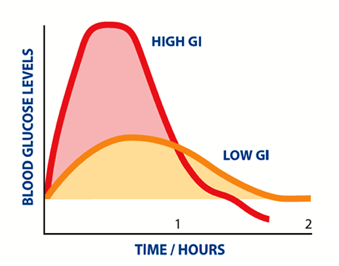
\includegraphics[width=3.53125in,height=2.77083in]{GI.png}}

\end{ajanlofig}

The \textbf{glycemic index} or \textbf{glycaemic index}
(\textbf{GI})\href{https://en.wikipedia.org/wiki/Glycemic_index\#cite_note-1}{{[}1{]}}
is a number associated with the carbohydrates in a particular type of
food that indicates the effect of these carbohydrates on a person's
blood \href{https://en.wikipedia.org/wiki/Glucose}{glucose} (also called
\href{https://en.wikipedia.org/wiki/Blood_sugar}{blood sugar}) level. A
value of 100 represents the
\href{https://en.wikipedia.org/wiki/Standard_(metrology)}{standard}, an
equivalent amount of pure
glucose.\href{https://en.wikipedia.org/wiki/Glycemic_index\#cite_note-glycemic1-2}{{[}2{]}}

The GI represents the rise in a person's blood sugar level two hours
after consumption of the food. The glycemic effects of foods depends on
a number of factors, such as the type of carbohydrate, physical
entrapment of the carbohydrate molecules within the food, fat and
protein content of the food and organic acids or their salts in the
meal. The GI is useful for understanding how the body breaks down
\href{https://en.wikipedia.org/wiki/Carbohydrate}{carbohydrates}\href{https://en.wikipedia.org/wiki/Glycemic_index\#cite_note-glycemicedge-3}{{[}3{]}}
and takes into account only the available carbohydrate (total
carbohydrate minus
\href{https://en.wikipedia.org/wiki/Dietary_fiber}{fiber}) in a food.
Glycemic index does not predict an individual's glycemic response to a
food, but can be used as a tool to assess the insulin response burden of
a food, averaged across a studied population. Individual responses vary
greatly.\href{https://en.wikipedia.org/wiki/Glycemic_index\#cite_note-ZeeviKorem2015-4}{{[}4{]}}

\end{ajanlo}

\hypertarget{alkalmazas}{%
\subsubsection{Alkalmazás}\label{alkalmazas}}

\begin{allitas}

Állítás:\\
legyenek \(X\), \(Y\) normált terek, \(\Omega \subset X\) tartomány
(azaz nyílt és összefüggő) \(\left. \Leftrightarrow\Omega \right.\)
nyílt és bármely két pontja összeköthető egy \(\Omega\)-ban haladó
törött vonallal. Tfh \(\left. f:\Omega\rightarrow Y \right.\) és \(f\)
differenciálható \(\Omega\) minden pontjában és
\(\left. f'\left( x \right) = 0,\forall x \in \Omega\Rightarrow f \right.\)
állandó.

\end{allitas}

\begin{bizonyitas}

Bizonyítás:\\
Legyen \(x_{1} \in \Omega,x_{2} \in \Omega\) tetszőleges. Belátjuk, hogy
\(f\left( x_{1} \right) = f\left( x_{2} \right) \in Y\). Kössük össze az
\(x_{1}\) és \(x_{2}\) pontokat egy \(\Omega\)-ban haladó törött
vonallal! A töréspontok legyenek
\(x_{1},\xi_{1},\xi_{2},...,\xi_{k},x_{2}\). Először alkalmazzuk a
Lagrange-egyenlőtlenséget \(L\left( {x_{1},\xi_{1}} \right)\)-re!
\[\left. \left\| {f\left( \xi_{1} \right) - f\left( x_{1} \right)} \right\| \leq \sup\limits_{\eta_{1} \in L{({x_{1},\xi_{1}})}}\left\| {f'\left( \eta_{1} \right)\left( {\xi_{1} - x_{1}} \right)} \right\| = 0\Rightarrow f\left( \xi_{1} \right) = f\left( x_{1} \right) \right..\]
Alkalmazva \(L\left( {\xi_{1},\xi_{2}} \right)\)-re,
\(L\left( {\xi_{2},\xi_{3}} \right)\)-ra,\ldots{},
\(L\left( {\xi_{k},x_{2}} \right)\)-re, kapjuk, hogy
\[\left. f\left( \xi_{1} \right) = f\left( \xi_{2} \right),f\left( \xi_{2} \right) = f\left( \xi_{3} \right),...,f\left( \xi_{k} \right) = f\left( x_{2} \right)\Rightarrow f\left( x_{1} \right) = f\left( x_{2} \right) \right..\]
■

\end{bizonyitas}

\hypertarget{fuggvenysorok-es-sorozatok-es-derivalasa}{%
\subsubsection{Függvénysorok és sorozatok és
deriválása}\label{fuggvenysorok-es-sorozatok-es-derivalasa}}

Legyenek
\(\left. f_{k}:\left\lbrack {a,b} \right\rbrack\rightarrow{\mathbb{R}} \right.\),
egyszerűség kedvéért folytonos függvények, \(k \in {\mathbb{N}}\). Tfh
\(\forall x \in \left\lbrack {a,b} \right\rbrack\) esetén
\(\underset{k\rightarrow\infty}{\lim}f_{k}\left( x \right) = f\left( x \right)\).
Ekkor mondtuk, hogy \(\left( f_{k} \right)\) függvény sorozat pontonként
tart egy \(f\) függvényhez.

\begin{megj_extra}

Kérdés: ebből következik-e, hogy
\(\underset{k\rightarrow\infty}{\lim}{\int\limits_{a}^{b}{f_{k}\left( x \right)dx}} = {\int\limits_{a}^{b}{f\left( x \right)dx}}\)
? Általában nem. Pl.:
\(f_{k}\left( x \right): = \left\{ \begin{array}{l} {x/\left( {1/2k} \right)\text{~ha~0} \leq x \leq 1/2k} \\ {- x/\left( {1/2k} \right) + 2k\text{~ha~}1/2k < x \leq 1/k} \\ {0\text{~egyébként}} \\ \end{array} \right.\)

\end{megj_extra}

\begin{tetel_extra}

Tétel:\\
Egy
\(\left. f_{k}:\left\lbrack {a,b} \right\rbrack\rightarrow{\mathbb{R}},f_{k} \in C\left\lbrack {a,b} \right\rbrack \right.\)
és \(\left. \left( f_{k} \right)\rightarrow f \right.\) egyenletesen
(\(\left. \Rightarrow f \in C\left\lbrack {a,b} \right\rbrack \right.\)).
Ekkor
\(\underset{k\rightarrow\infty}{\lim}{\int\limits_{a}^{b}{f_{k}\left( x \right)dx}} = {\int\limits_{a}^{b}{f\left( x \right)dx}}\).

\end{tetel_extra}

\begin{biz_extra}

Bizonyítás:\\
\(\underset{k\rightarrow\infty}{\lim}\left| {{\int\limits_{a}^{b}{f_{k}\left( x \right)dx}} - {\int\limits_{a}^{b}{f\left( x \right)dx}}} \right| = 0\)
ezt kellene belátni.
\(\left| {{\int\limits_{a}^{b}{f_{k}\left( x \right)dx}} - {\int\limits_{a}^{b}{f\left( x \right)dx}}} \right| = \left| {\int\limits_{a}^{b}{\left\lbrack {f_{k}\left( x \right) - f\left( x \right)} \right\rbrack dx}} \right| \leq {\int\limits_{a}^{b}{\left| {f_{k}\left( x \right) - f\left( x \right)} \right|dx}}\).
Mivel \(\left. \left( f_{k} \right)\rightarrow f \right.\) egyenletesen
\(\left. \Rightarrow\forall\varepsilon > 0\exists k_{0}:k > k_{0}\Rightarrow\left| {f_{k}\left( x \right) - f\left( x \right)} \right| < \varepsilon,\forall x \in \left\lbrack {a,b} \right\rbrack \right.\).
Így
\(\int\limits_{a}^{b}{\left| {f_{k}\left( x \right) - f\left( x \right)} \right|dx < \varepsilon \cdot \left( {b - a} \right)}\),
ebből következik a tétel állítása. ■

\end{biz_extra}

\begin{all_extra}

Állítás:\\
Legyen
\(\left. g_{j}:\left\lbrack {a,b} \right\rbrack\rightarrow{\mathbb{R}},g_{j} \in C\left\lbrack {a,b} \right\rbrack \right.\),
\({\sum\limits_{j = 1}^{\infty}g_{j}} = f\) sor egyenletesen konvergens
(vagyis ha a részletösszegek sorozata egyenletesen konvergál \(f\)-hez,
ekkor amúgy \(f\) folytonos)
\(\left. \Rightarrow{\sum\limits_{j = 1}^{\infty}{{\int\limits_{a}^{b}{g_{j}\left( x \right)dx}} = {\int\limits_{a}^{b}{f\left( x \right)dx}}}} \right.\).

\end{all_extra}

\begin{tetel_extra}

Tétel:\\
Tfh \(\left. f_{k}:\left( {a,b} \right)\rightarrow{\mathbb{R}} \right.\)
függvény folytonosan differenciálható, továbbá
\(\left. \left( {f_{k}'} \right)\rightarrow g \right.\) egyenletesen
\(\left( {a,b} \right)\)-n, továbbá egy alkalmas
\(c \in \left( {a,b} \right)\) helyre
\(\underset{k\rightarrow\infty}{\lim}f_{k}\left( c \right) = \alpha\)
véges. Ebből következik, hogy
\(\left. \left( f_{k} \right)\rightarrow f \right.\) egyenletesen
\(\left( {a,b} \right)\)-n, \(f\) folytonosan differenciálható és
\(f'\left( x \right) = \underset{k\rightarrow\infty}{\lim}\left\lbrack {f_{k}'\left( x \right)} \right\rbrack\).

\end{tetel_extra}

\begin{biz_extra}

Bizonyítás:\\
Alkalmazzuk a Newton-Leibniz formulát az \(f_{k}\) folytonosan
differenciálható függvényekre, \(x \in \left( {a,b} \right)\) rögzített.
\(\left. f_{k}\left( x \right) - f_{k}\left( c \right) = {\int\limits_{c}^{x}{f_{k}'\left( t \right)dt}}\Rightarrow f_{k}\left( x \right) = {\int\limits_{c}^{x}{f_{k}'\left( t \right)dt}} + f_{k}\left( c \right)\rightarrow{\int\limits_{c}^{x}{g\left( t \right)dt}} + \alpha \right.\),
mert
\(\left. f_{k}'\left( t \right)\rightarrow g\left( t \right) \right.\)
egyenletesen, \(t \in \left\lbrack {x,c} \right\rbrack\) vagy
\(t \in \left\lbrack {c,x} \right\rbrack\). Továbbá \(f_{k}\)
egyenletesen tart
\(\underset{f{(x)}}{\underset{\}\ }{\left\lbrack {\int\limits_{c}^{x}{g\left( t \right)dt + \alpha}} \right\rbrack}}\)-hoz,
ugyanis
\(\left| {f_{k}\left( x \right) - f\left( x \right)} \right| = \left| {\left\lbrack {{\int\limits_{c}^{x}{f_{k}'\left( t \right)dt}} + f_{k}\left( c \right)} \right\rbrack - \left\lbrack {\int\limits_{c}^{x}{g\left( t \right)dt + \alpha}} \right\rbrack} \right| \leq \left| {\int\limits_{c}^{x}{\left( {f_{k}'\left( t \right) - g\left( t \right)} \right)dt}} \right| + \underset{< \varepsilon\text{~ha~}k > k_{0}}{\underset{\}\ }{\left| {f_{k}\left( c \right) - \alpha} \right|}} \leq\)
\(\leq \left| {x - c} \right| \cdot \underset{< \varepsilon\text{~ha~k} > k_{1}}{\underset{\}\ }{\sup\left( \left| {f_{k}'\left( t \right) - g\left( t \right)} \right| \right)}} + \varepsilon \leq \left( {b - a} \right)\varepsilon + \varepsilon\)
és
\(\left. k \geq \max\left\{ {k_{0},k_{1}} \right\}\Rightarrow\left( f_{k} \right)\rightarrow f \right.\)
egyenletesen \(\left( {a,b} \right)\)-n. Kellett, hogy
\(\left( {b - a} \right)\) véges legyen!
\(\left. f\left( x \right) = {\int\limits_{c}^{x}{g\left( t \right)dt}} + \alpha\Rightarrow f'\left( x \right) = g\left( x \right),\forall x \in \left( {a,b} \right) \right.\).
■

\end{biz_extra}

\begin{tetel}

Tétel:\\
Tfh
\(\left. \phi_{j}:\left( {a,b} \right)\rightarrow{\mathbb{R}} \right.\)
folytonosan differenciálható.
\({\sum\limits_{j = 1}^{\infty}{\phi_{j}'}} = g\) egyenletesen
konvergens \(\left( {a,b} \right)\)-n, továbbá
\(\exists c \in \left( {a,b} \right):{\sum\limits_{j = 1}^{\infty}{\phi_{j}\left( c \right)}} = \alpha\)
véges. Ekkor \(\sum\limits_{j = 1}^{\infty}\phi_{j}\) egyenletesen
konvergens \(\left( {a,b} \right)\)-n,
\(f: = {\sum\limits_{j = 1}^{\infty}\phi_{j}}\) függvény
differenciálható \(\left( {a,b} \right)\)-n és
\(f'\left( x \right) = {\sum\limits_{j = 1}^{\infty}{\phi_{j}'\left( x \right)}},\forall x \in \left( {a,b} \right)\).

\end{tetel}

\begin{bizonyitas}

Bizonyítás:\\
\(f_{k} = {\sum\limits_{j = 1}^{k}\phi_{j}}\) \ldots{}

\end{bizonyitas}

\begin{tetel}

Tétel (Cauchy-féle középérték tétel):\\
\(\left. f,g:\left\lbrack {a,b} \right\rbrack\rightarrow{\mathbb{R}} \right.\),
folytonosak, \(\left( {a,b} \right)\)-n differenciálhatóak és
\(g'\left( x \right) \neq 0,\forall x \in \left( {a,b} \right)\). Ekkor
\(\exists\xi \in \left( {a,b} \right):\frac{f\left( b \right) - f\left( a \right)}{g\left( b \right) - g\left( a \right)} = \frac{f'\left( \xi \right)}{g'\left( \xi \right)}\).
(Ha \(g\left( x \right) = x\), akkor ez a Lagrange-féle .)

\end{tetel}

\begin{bizonyitas}

Bizonyítás:\\
\(g\left( b \right) - g\left( a \right) \neq 0\), ugyanis ha
\(g\left( b \right) - g\left( a \right) = 0\) lenne, akkor a Rolle-tétel
szerint \(g\) függvényre
\(\exists\eta \in \left( {a,b} \right):g'\left( \eta \right) = 0\).
Legyen
\(F\left( x \right): = f\left( x \right) - \frac{f\left( b \right) - f\left( a \right)}{g\left( b \right) - g\left( a \right)}\left\lbrack {g\left( x \right) - g\left( a \right)} \right\rbrack\).
Ekkor \(F\) folytonos \(\left\lbrack {a,b} \right\rbrack\)-n és
differenciálható \(\left( {a,b} \right)\)-n,
\(F\left( a \right) = f\left( a \right)\),
\(F\left( b \right) = f\left( b \right) - \frac{f\left( b \right) - f\left( a \right)}{g\left( b \right) - g\left( a \right)}\left\lbrack {g\left( b \right) - g\left( a \right)} \right\rbrack = f\left( a \right)\).
\(\left. F\left( a \right) = F\left( b \right)\Rightarrow \right.\)
Rolle-tétel segítségével
\(\exists\xi \in \left( {a,b} \right):F'\left( \xi \right) = 0\), azaz
\(0 = F'\left( \xi \right) = f'\left( \xi \right) - \frac{f\left( b \right) - f\left( a \right)}{g\left( b \right) - g\left( a \right)}g'\left( \xi \right)\).
■

\end{bizonyitas}

\hypertarget{l-hopital-szabaly}{%
\subsubsection{L' Hôpital szabály}\label{l-hopital-szabaly}}

\begin{tetel}

Tétel (L' Hôpital (avagy L' Hospital) szabály alapesete):\\
Tfh \(f\), \(g\) értelmezve van és differenciálható
\(a \in {\mathbb{R}}\) egy környezetében (\(a\)-ban nem is kell),
továbbá
\(\underset{x\rightarrow a}{\lim}f\left( x \right) \equiv \underset{a}{\lim}f = 0\)
és \(\underset{b}{\lim}g = 0\). Ekkor
\(\underset{a}{\lim}\frac{f}{g} = \underset{a}{\lim}\frac{f'}{g'}\), ha
létezik ez utóbbi.

\end{tetel}

\begin{bizonyitas}

Bizonyítás:\\
értelmezzük az \(f\) és \(g\) függvényt \(a\)-ban!
\(f\left( a \right): = 0\), \(g\left( a \right): = 0\). Ezért \(f\),
\(g\) folytonosak \(a\) egy környezetében és deriválhatók is \(x\)
kivételével, \(g'\left( x \right) \neq 0\). Alkalmazzuk a Cauchy-féle
középérték-tételt: \(a\) környezetében levő \(x\) pont és \(a\) által
meghatározott intervallumra
\(\left. \exists\xi \in \left( {a,b} \right):\frac{f\left( x \right)}{g\left( x \right)} = \frac{f\left( x \right) - f\left( a \right)}{g\left( x \right) - g\left( a \right)} = \frac{f'\left( \xi \right)}{g'\left( \xi \right)}\Rightarrow x\rightarrow a \right.\)
esetén
\(\left. \xi\rightarrow a\Rightarrow\underset{x\rightarrow a}{\lim}\frac{f\left( x \right)}{g\left( x \right)} = \underset{\xi\rightarrow a}{\lim}\frac{f'\left( \xi \right)}{g'\left( \xi \right)} \right.\),
ha ez utóbbi létezik. ■

\end{bizonyitas}

Általánosítások:

\begin{enumerate}
\def\labelenumi{\arabic{enumi}.}
\tightlist
\item
  \(a: = \pm \infty\) és
  \(\underset{a}{\lim}f = 0,\underset{a}{\lim}g = 0\), ekkor is igaz,
  hogy
  \(\underset{a}{\lim}\frac{f}{g} = \underset{a}{\lim}\frac{f'}{g'}\) ,
  ha ez utóbbi létezik .
\item
  \(\underset{a}{\lim}f = \pm \infty\) és
  \(\underset{a}{\lim}g = \pm \infty\) esetén hasonló állítás.
\end{enumerate}

\hypertarget{hatvanysorok-integralasa-es-derivalasa}{%
\subsubsection{Hatványsorok integrálása és
deriválása}\label{hatvanysorok-integralasa-es-derivalasa}}

\(\sum\limits_{k = 0}^{\infty}{c_{k}\left( {x - a} \right)^{k}}\),
\(a,x \in {\mathbb{R}}\) ezt nevezzük \(x\)-nek \(a\) körüli
hatványsornak. Ez egy speciális függvénysor. Legyen ennek a konvergencia
sugara \(R\) ! Tudjuk, hogy \(\left| {x - a} \right| < R\) esetén a
hatványsor konvergens \(x\)-ben. Azt is tudjuk, hogy
\(\forall\delta > 0\) esetén a hatványsor egyenletesen konvergens
\(\left\lbrack {a - R + \delta,a + R - \delta} \right\rbrack\)
intervallumon.

\begin{tetel}

Tétel:\\
Legyen a hatványsor konvergencia sugara \(R > 0\) és \(R \leq \infty\).
Ekkor egyrészt tetszőleges
\(\left\lbrack {c,d} \right\rbrack \subset \left( {a - R,a + R} \right)\)
esetén a hatványsor tagonként integrálható, vagyis
\({\int\limits_{c}^{d}{{\sum\limits_{k = 0}^{\infty}{c_{k}\left( {x - a} \right)^{k}}}dx}} = {\sum\limits_{k = 0}^{\infty}{\int\limits_{c}^{d}{c_{k}\left( {x - a} \right)^{k}dx}}}\).

\end{tetel}

\begin{tetel}

Tétel:\\
Legyen a hatványsor konvergencia sugara \(R > 0\) és \(R \leq \infty\).
Ekkor \(\left| {x - a} \right| < R\) esetén a hatványsor \(x\)-ben
tagonként deriválható:
\[{\left( {\sum\limits_{k = 0}^{\infty}{c_{k}\left( {x - a} \right)^{k}}} \right)' = {\sum\limits_{k = 0}^{\infty}{\left( {c_{n}\left( {x - a} \right)^{k}} \right)'}}}.\]

\end{tetel}

\begin{bizonyitas}

Bizonyítás:\\
Alkalmazzuk a függvénysorok tagonkénti deriválásáról szóló tételt!
Világos, hogy a hatványsor tagjai folytonosak, akárhányszor
differenciálhatóak. Kérdés: mi a tagok deriváltjaiból alkotott
hatványsor konvergencia sugara? Látható, hogy ugyanaz. A derivált sor
\(k\)-adik tagja: \(c_{k}k\left( {x - a} \right)^{k - 1}\), erre ugyanaz
a konvergencia sugár adódik. Tehát a deriváltakból álló sor egyenletesen
konvergens \(\left\lbrack {c,d} \right\rbrack\)-n ha
\(\left\lbrack {c,d} \right\rbrack \subset \left( {a - R,a + R} \right)\),
\(\left| {x - a} \right| < R\), \(\left\lbrack {c,d} \right\rbrack\)-t
megválaszthatjuk úgy, hogy \(x \in \left\lbrack {c,d} \right\rbrack\). ■

\end{bizonyitas}

\hypertarget{taylor-formula}{%
\paragraph{Taylor-formula}\label{taylor-formula}}

Tfh egy hatványsor konvergencia sugara \textgreater{} 0,
\(f\left( x \right) = {\sum\limits_{k = 0}^{\infty}{c_{k}\left( {x - a} \right)^{k}}}\),
\(\left| {x - a} \right| < R > 0\). (Definíció szerint itt
\(0^{0} = 1\).)\\
Az előbbiek szerint \(\left| {x - a} \right| < R\) esetén\\
\(\begin{array}{l} {f'\left( x \right) = {\sum\limits_{k = 0}^{\infty}{c_{k}k\left( {x - a} \right)^{k - 1}}}} \\ {f''\left( x \right) = {\sum\limits_{k = 0}^{\infty}{c_{k}k\left( {k - 1} \right)\left( {x - a} \right)^{k - 2}}}} \\  \vdots \\ {f^{(j)}\left( x \right) = {\sum\limits_{k = 0}^{\infty}{c_{k}k\left( {k - 1} \right)\left( {k - 2} \right)...\left( {k - j + 1} \right)\left( {x - a} \right)^{k - j}.}}} \\ \end{array}\)\\
Ekkor
\(\left. f^{(j)}\left( a \right) = c_{j} \cdot j\left( {j - 1} \right)\left( {j - 2} \right)...2 \cdot 1 = c_{j}j!\Rightarrow c_{j} = \frac{f^{(j)}\left( a \right)}{j!} \right.\).

\begin{allitas}

Állítás:\\
Ha
\(f\left( x \right) = {\sum\limits_{k = 0}^{\infty}\left. c_{k}\left( {x - a} \right)^{k},\left| {x - a} \right| < R > 0\Rightarrow c_{k} = \frac{f^{(k)}\left( a \right)}{k!} \right.}\).

\end{allitas}

Speciális eset, ha \(f\) polinom, azaz \(f = P_{N}\) ( \(N\) -edfokú
polinom), vagyis
\(f = {\sum\limits_{k = 0}^{N}{c_{k}\left( {x - a} \right)^{k}}}\),
ekkor \(c_{k} = \frac{P^{(k)}\left( a \right)}{k!}\), más szóval
\(P\left( x \right) = {\sum\limits_{k = 0}^{N}{\frac{P^{(k)}\left( a \right)}{k!}\left( {x - a} \right)^{k}}}\).

\begin{definicio}

Definíció:\\
Tfh egy \(f\) függvény \(a\) egy környezetében akárhányszor
differenciálható! Ekkor a
\({\sum\limits_{k = 0}^{N}\frac{f^{(k)}\left( a \right)}{k!}}\left( {x - a} \right)^{k}\)
polinomot az \(f\) függvény \(a\) pont körül felírt \(N\) -edfokú
Taylor-polinomjának, a
\(\sum\limits_{k = 0}^{\infty}{\frac{f^{(k)}\left( a \right)}{k!}\left( {x - a} \right)^{k}}\)
hatványsort pedig az \(f\) függvény \(a\) pont körüli Taylor-sorának
nevezzük.

\end{definicio}

\hypertarget{taylor-formula-lagrange-fele-maradektaggal}{%
\subsubsection{Taylor-formula Lagrange-féle
maradéktaggal}\label{taylor-formula-lagrange-fele-maradektaggal}}

Motiváció: Egy \(f\) függvény \(a\) pont körül felírt Taylor-sor mikor
(milyen \(x\) értékekre) adja magát az \(f\) függvényt?

\begin{tetel}

Tétel:\\
Tfh \(f\) függvény \(N\) +1-szer differenciálható \(a\) egy
környezetében. Ebben a környezetben fekvő tetszőleges \(x\) pontjára
\(f\left( x \right) = {\sum\limits_{k = 0}^{N}{\frac{f^{(k)}\left( a \right)}{k!}\left( {x - a} \right)^{k} +}}\frac{f^{({N + 1})}\left( \xi \right)}{\left( {N + 1} \right)!}\left( {x - a} \right)^{N + 1}\),
alkalmasan választott \(\xi \in \left( {x,a} \right)\) elemre.

\end{tetel}

\begin{megjegyzes}

Megjegyzés:\\
\(N = 0\) esetén megkapjuk a Lagrange-féle középértéktételt.

\end{megjegyzes}

\begin{bizonyitas}

Bizonyítás:\\
Jelölje
\(g\left( x \right): = f\left( x \right) - {\sum\limits_{k = 0}^{N}{\frac{f^{(k)}\left( a \right)}{k!}\left( {x - a} \right)^{k}}} = f\left( x \right) - P\left( x \right)\).
Ekkor \(g\left( a \right) = f\left( a \right) - P\left( a \right)\), de
\(P\left( a \right) = f\left( a \right)\), így
\(g\left( a \right) = 0\). Továbbá
\(g'\left( a \right) = f'\left( a \right) - P'\left( a \right)\), node
\(f'\left( a \right) = P'\left( a \right)\), így
\(g'\left( a \right) = 0\) \ldots{}
\(g^{(n)}\left( a \right) = f^{(n)}\left( a \right) - P^{(n)}\left( a \right) = 0\).
Tekintsük:
\(\frac{g\left( x \right)}{\left( {x - a} \right)^{N + 1}} = \frac{g\left( x \right) - g\left( a \right)}{\left( {x - a} \right)^{N + 1} - \left( {a - a} \right)^{N + 1}} = \frac{g'\left( \xi \right)}{\left( {n + 1} \right)\left( {\xi_{1} - a} \right)^{N}}\),
felhasználva a Cauchy-féle középérték tételt. További alkalmazása
segítségével \[\begin{aligned}
  \frac{{g\left( x \right)}}{{{{\left( {x - a} \right)}^{N + 1}}}} =  & \frac{{g'\left( {{\xi _1}} \right) - g'\left( a \right)}}{{\left( {N + 1} \right){{\left( {{\xi _1} - a} \right)}^N} - \left( {N + 1} \right){{\left( {a - a} \right)}^N}}} \\ 
   =  & \frac{{g''\left( {{\xi _2}} \right)}}{{\left( {N + 1} \right)N\left( {{\xi _2} - a} \right)}} \\ 
   =  & ... \\ 
   =  & \frac{{{f^{\left( {N + 1} \right)}}\left( {{\xi _{N + 1}}} \right)}}{{\left( {N + 1} \right)!}}, \\ 
\end{aligned} \] amelyből következik, hogy
\[\frac{{g\left( x \right)}}{{{{\left( {x - 1} \right)}^{N + 1}}}} = \frac{{{f^{\left( {N + 1} \right)}}\left( {{\xi _{N + 1}}} \right)}}{{\left( {N + 1} \right)!}}.\]
■

\end{bizonyitas}

Következmény: ha \(f\) akárhányszor differenciálható \(a\) egy
környezetében, és
\[\lim\limits_{N\rightarrow\infty}\frac{f^{({N + 1})}\left( \xi \right)}{\left( {N + 1} \right)!}\left( {x - a} \right)^{N + 1} = 0\]
\(\xi \in \left( {a,x} \right)\)-ben egyenletesen, akkor
\(\left. \Rightarrow f\left( x \right) = {\sum\limits_{k = 0}^{\infty}{\frac{f^{(k)}\left( a \right)}{k!}\left( {x - a} \right)^{k}}} \right.\),
vagyis ezesetben az \(a\) körüli Taylor-sor előállítja az \(f\) függényt
azon \(x\) értékekre, amelykre a fenti feltétel teljesül. Egyszerű,
elegendő (de nem szükséges) feltétel, ha
\(\xi \in \left( {a,x} \right)\),
\(\left| {f^{({n + 1})}\left( \xi \right)} \right|\) egyenletesen
korlátos, ugyanis
\(\underset{n\rightarrow\infty}{\lim}\frac{\left( {x - a} \right)^{n + 1}}{\left( {n + 1} \right)!} = 0\).

\begin{megjegyzes}

Megjegyzés:\\
Lehetséges, hogy \(f\) akárhányszor differenciálható, de a Taylor-sora
az \(a\) pont kivételével nem állítja elő a függvényt. Ilyen pl. az
alábbi. \[f\left( x \right) = \begin{cases}
0 & {\text{ha~}x = 0} \\
e^{- \frac{1}{x^{2}}} & \text{egyébként} \\
\end{cases}\] Ennek
\(\left. \underset{x\rightarrow 0}{\lim}f\left( x \right) = 0,\underset{x\rightarrow 0}{\lim}f'\left( x \right) = 0...\underset{x\rightarrow 0}{\lim}f^{(k)}\left( x \right) = 0,\forall k\Rightarrow f \right.\)
akárhányszor deriválható az \(a = 0\) helyen.
\(\underset{h\rightarrow 0}{\lim}\frac{f\left( h \right) - f\left( 0 \right)}{h - 0} = 0\),
tehát
\(\left. f'\left( 0 \right) = 0,f''\left( 0 \right) = 0...\Rightarrow f \right.\)
Taylor-sora 0, pedig \(f\left( x \right) > 0\) ha \(x \neq 0\).

\end{megjegyzes}

\begin{ajanlo}

\begin{ajanlofig}

\href{https://www.youtube.com/watch?v=o1Hbjq73-ME}{
\includegraphics[width=4.6875in,height=3.08333in]{potete.jpg}}

\end{ajanlofig}

\textbf{\emph{State buoni se potete}} is a
\href{https://en.wikipedia.org/wiki/List_of_Italian_films_of_1983}{1983}
\href{https://en.wikipedia.org/wiki/Cinema_of_Italy}{Italian}
\href{https://en.wikipedia.org/wiki/Historical_film}{historical}
\href{https://en.wikipedia.org/wiki/Comedy-drama}{comedy-drama} film
written and directed by
\href{https://en.wikipedia.org/wiki/Luigi_Magni}{Luigi Magni}. The film
is loosely based on real life events of Saint
\href{https://en.wikipedia.org/wiki/Philip_Neri}{Filippo
Neri}.\href{https://en.wikipedia.org/wiki/State_buoni_se_potete\#cite_note-80-89_m-z-1}{{[}1{]}}
For his musical score
\href{https://en.wikipedia.org/wiki/Angelo_Branduardi}{Angelo
Branduardi} won the
\href{https://en.wikipedia.org/wiki/David_di_Donatello}{David di
Donatello} for
\href{https://en.wikipedia.org/wiki/David_di_Donatello_for_Best_Score}{best
score} and the \href{https://en.wikipedia.org/wiki/Silver_Ribbon}{Silver
Ribbon} in
\href{https://en.wikipedia.org/wiki/Nastro_d\%27Argento_for_Best_Score}{the
same
category}.\href{https://en.wikipedia.org/wiki/State_buoni_se_potete\#cite_note-premi-2}{{[}2{]}}

\end{ajanlo}

\end{document}
